\documentclass[12pt,oneside,openany,a4paper,%..... Layout
               afrikaans, english,%.............. Global language selection
               ]{memoir}

 \usepackage[masters-t,%.......................... Master thesis
             goldenblock,%........................ A5 type block (or a5block or wide)
            ]{usthesis}%.......................... US thesis style with memoir

%
% PLEASE read the USthesis documentation for the class options
% and how to set line and paragraph spacing
%

%==== MY PACKAGES ====================================================
\usepackage{caption}
\usepackage{subcaption}
\usepackage[upgrade=true]{acro}

%==== Language setup ================================================
 \usepackage[latin1]{inputenc}%................... Recognizes �, �, etc
 \usepackage{babel}%.............................. Language setup

%==== Math setup ====================================================
 \usepackage{amsmath}%............................ Advanced math (before fonts)
 %\usepackage{amssymb}%............................ AMS Symbol fonts

%==== Font setup (default is Computer Modern) =======================
 \usepackage[T1]{fontenc}%........................ Type 1 fonts
 %\usepackage{fourier}
 \usepackage{textcomp}%........................... Additional text character
 \usepackage{bm}%................................. Bold math symbols (after fonts)

%==== Ref's, Bib's and Nomencl ======================================
 \usepackage{usnomencl}%.......................... List of symbols (in usthesis pack)
 \usepackage[square, numbers]{natbib}%.............................. Bibliography    (in usthesis pack)

    \bibliographystyle{IEEEtranN}
    \renewcommand\bibfont{\small}
    \def\BIBand{and}

    %% For usmeg-a, the bib is a list of references. If you
    %% are using usmeg-n comment out the following lines
    \addto{\captionsafrikaans}{\renewcommand{\bibname}{Lys van Verwysings}}
    \addto{\captionsenglish}{\renewcommand{\bibname}{List of References}}

%==== Graphics and Color ============================================
\usepackage{graphicx}%........................... Graphicx loaded in usthesis
\usepackage{color}%.............................. Color setup
\usepackage{eso-pic}%............................ Shipout commands for watermark
    \newcommand*{\WaterMark}[2][0.15\paperwidth]{%
        \AddToShipoutPicture*{\AtTextCenter{%
                \parbox[c]{0pt}{\makebox[0pt][c]{%
                    \includegraphics[width=#1]{#2}}}}}}



%==== Local Defs ====================================================
\makeatletter

%
% Please insert user defined commands here
% and NOT in the document itself!
%

\makeatother

%==== TITLE PAGE ====================================================
\title{\bfseries
       \AorE{%-- Afrikaans ------------------------------------------
             TODO: Insert Afrikaans Title Here\\[1ex]
             \normalfont\small\itshape
             (``Grid-Based Coverage Path Planning with Multiple UAVs for Search and Rescue Applications'')
            }{%-- English -------------------------------------------
             Grid-Based Coverage Path Planning with Multiple UAVs for Search and Rescue Applications
            }}

\author{W.\ Botes}{Welri Botes}

\degree{\AorE{MIng (EE)}{MEng (EE)}}
       {\AorE{Magister in Ingenieurswese (Elektries en Elektronies)}
             {Master of Engineering (Electrical and Electronic)}}

\address{\AorE{%-- Afrikaans ----------------------------------------
        Departement Elektries en Elektroniese Ingenieurswese,\\
        Universiteit van Stellenbosch,\\
        Privaatsak X1, Matieland 7602, Suid Afrika.%
             }{%-- English ------------------------------------------
        Department of Electrical and Electronic Engineering,\\
        University of Stellenbosch,\\
        Private Bag X1, Matieland 7602, South Africa.
             }}

\faculty{\AorE{Fakulteit Ingenieurswese}%
              {Faculty of Engineering}}

\supervisor{Dr\ JAA\ Engelbrecht}

\cosupervisor{Mr\ JC \ Schoeman}

\setdate{09}{2021}

%\SetSponsor{The financial assistance of the National Research Foundation (NRF)
%    towards this research is hereby acknowledged. Opinions expressed and
%    conclusions arrived at, are those of the author and are not necessarily to
%    be attributed to the NRF.}


%====================================================================
%     MAIN DOCUMENT
%====================================================================
\maxsecnumdepth{subsubsection}
\maxtocdepth{section}

\begin{document}

%==== Front matter ==================================================
 \frontmatter
 \WaterMark{UScrest-WM}
 \TitlePage

 \DeclarationDate{2021/08/30}
 \DeclarationPage

 \begin{abstract}[english]%===================================================
Vibrating a tillage tool is an effective way of reducing the draft force
required to pull it through the soil. The degree of draft force reduction is
dependent on the combination of operating parameters and soil conditions. It
is thus necessary to optimize the vibratory implement for different
conditions.

Numerical modelling is more flexible than experimental testing and analytical
models, and less costly than experimental testing. The Discrete Element
Method (DEM) was specifically developed for granular materials such as soils
and can be used to model a vibrating tillage tool for its design and
optimization. The goal was thus to evaluate the ability of DEM to model a
vibratory subsoiler and to investigate the cause of the draft force
reduction.

The DEM model was evaluated against data ...
\end{abstract}


\begin{abstract}[afrikaans]%=================================================
Om `n tand implement te vibreer is `n effektiewe manier om die trekkrag, wat
benodig word om dit deur die grond te trek, te verminder. Die graad van krag
vermindering is afhanklik van die kombinasie van werks parameters en die
grond toestand. Dus is dit nodig om die vibrerende implement te optimeer vir
verskillende omstandighede.

Numeriese modulering is meer buigsaam en goedkoper as eksperimentele
opstellings en analitiese modelle. Die Diskrete Element Metode (DEM) was
spesifiek vir korrelrige materiaal, soos grond, ontwikkel en kan gebruik word
vir die modellering van `n vibrerende implement vir die ontwerp en optimering
daarvan. Die doel was dus om die vermo� van DEM om 'n vibrerende skeurploeg
the modelleer, te evalueer, en om die oorsaak van die krag vermindering te
ondersoek.

Die DEM model was ge�valueer teen data ...
\end{abstract}


\chapter{Acknowledgements}%==================================================

I would like to express my sincere gratitude to the following people
and organisations ...


\chapter{Dedications}%=======================================================
 \vfill
 \begin{Afr}
 \begin{center}\itshape
    Hierdie tesis word opgedra aan ...
 \end{center}
 \end{Afr}
 \vfill
 \clearpage

%============================================================================
\endinput


 \tableofcontents
 \clearpage

 \setcounter{lofdepth}{2}
 \listoffigures
 \clearpage

 \listoftables
 \clearpage

 \chapter{Nomenclature}

\begin{Nomencl}
 \NomGroup{Constants}%-----------------------------------------------
   % TODO: Remove the line below and decide if you want to remove constants entirely
   \item[$\mathrm{g} = $] $\mathrm{9.81\,m/s^2}$

 \NomGroup{Variables}%-----------------------------------------------
	\item[$\phi$] \UnitLine{Camera sensor to lens angle}{\deg}
	\item[$H$] \UnitLine{Height from camera lens to ground}{m}
	\item[$FOV$] \UnitLine{Field of view (on ground)}{m}
	\item[$AOV$] \UnitLine{Camera angle of view}{\deg}
	\item[$f$] \UnitLine{Camera focal length}{mm}
	\item[$h_{len}$] \UnitLine{Camera sensor height}{mm}
	\item[$w_{len}$] \UnitLine{Camera sensor width}{mm}
	\item[$GSD$] \UnitLine{Ground sampling distance}{cm/px}

 \NomGroup{Subscripts}%----------------------------------------------
   \item[$x$] The x dimension
   \item[$y$] The y dimension
  
\end{Nomencl}

\endinput

 
  
 \DeclareAcronym{uav}{short = UAV, long = Unmanned Aerial Vehicle}
 \DeclareAcronym{ugv}{short = UGV, long = Unmaned Ground Vehicle}
 \DeclareAcronym{cpp}{short = CPP, long = Coverage Path Planning}
 \DeclareAcronym{mcpp}{short = MCPP, long = Multi-Robot Coverage Path Planning}
 \DeclareAcronym{sar}{short = SAR, long = Search and Rescue}
 \DeclareAcronym{aov}{short = AOV, long = Angle of View}
 \DeclareAcronym{fov}{short = FOV, long = Field of View}
 \DeclareAcronym{gsd}{short = GSD, long = Ground Sampling Distance}
  
 \chapter{Acronyms}
	\printacronyms[heading=Acronyms,template=description,display=all,sort=true]
 
%==== Main document =================================================
\mainmatter

   \setsecnumdepth{subsubsection}
%   \numberwithin{equation}{section}
%   \numberwithin{figure}{chapter}
%   \numberwithin{table}{chapter}

\chapter{Introduction}
\label{chp:intro}


%%%%%%%%%%%%%%%%%%%%%%%%%%%%%%%%%%%%%%%%%%%%%%%%%%%%%%%%%%%%%%%%%%%%%%%
\section{Background}

Unmanned Aerial Vehicles (UAVs) are a technology that have gained popularity in various applications recently\cite{CPP-Survey-2019}. Originally, UAVs required a ground pilot to manoeuvre them, but are becoming an increasingly automated technology. Applications where UAV automation has been used include, but are not limited to, structure inspections\cite{Guerrero2013}, smart farming\cite{Lottes2017}, disaster management\cite{Maza2011}, power line inspections\cite{Chang2017}, surveillance\cite{Basilico2015} and wildfire tracking\cite{Pham2017}.

Most of the research mentioned was done on the premise of using multi-rotor UAVs, quad-rotor vehicles in particular. It is important to note that the term UAVs also encompasses other aircraft types, like single rotor and fixed wing UAVs. Hybrids also exist that contain both rotary-wing and fixed-wing components\cite{CPP-Survey-2019}.

Using UAVs poses a considerable advantage in applications like the ones mentioned when compared to unmanned ground vehicles (UGVs). Their capacity to fly over landscapes and around three dimensional structures makes their potential functionality increase substantially. Relatively high altitude flying is a key reason why they are well suited to the application suggested in this paper, which is coverage path planning for search and rescue missions.

Coverage path planning (CPP) is a variant of the general motion planning problem. Originally, motion planning algorithms were predominantly used to find solutions for start-goal problems\cite{Choset2001}. This implies finding a sequence of actions to get an object from some starting state to some goal state. An example would be finding a sequence of movements to get a robotic arm from one orientation to another. In the context of path planning it means getting an agent, a UAV for example, from some starting position to some goal position in an environment\cite{Lynch2017}.

Coverage path planning is different from start-goal path planning in that it tries to determine a path for an agent to pass over all points in an environment\cite{Choset2001}. It can be used with ground vehicles, for example, to automate field machines for smart farming\cite{Hameed2014}. Further examples include vacuum cleaning robots, spray painting robots\cite{Atkar2005}, window cleaning robots\cite{Mir-Nasiri2018} and automated lawn mowers\cite{Arkin1999}. For underwater vehicles it can be used for the inspection of difficult to reach underwater structures\cite{Englot2012}. 

Furthermore, there have been developments in the use of UAVs to perform automated search and rescue operations. Perhaps the most notable example is a project by DroneSAR where they use DJI drones to perform search and rescue tasks. Their implementation includes a mobile app that allows the user to designate a search area manually\cite{DroneSAR01}. This is called off-line coverage, where the environment is known prior to the path planning step. The entire path is computed before being performed by the UAV. Online coverage allows the path to change or be computed during path execution. Often times the environment is not known a priori\cite{CPP-Survey-2019}. 

There is a downside regarding computation time in an off-line approach, but complete coverage is more achievable in an off-line approach. Online approaches are very useful for situations where the environment is constantly changing or there is very little known about the environment. Search and rescue operations often span large areas and UAVs fly above most ground obstacles. Therefore, it is realistic to assume the environment can be mapped prior to the search operation, especially since complete coverage is rather important in a search and rescue operation.\cite{CPP-Survey-2013}

DroneSAR uses one drone per search and rescue operation. 

\section{Objectives}

The main objective of this thesis was to develop a coverage path planning algorithm that utilises multiple UAVs to search a known environment. This research is intended to be applicable to search and rescue operations.\linebreak
\cite{CPP-Survey-2019}


\section{Methodology}


\section{Scope of the Research}


\section{Thesis Structure}
% Later
% !TeX spellcheck = en_US
\chapter{Literature Review}
\label{chp:back}
% Why use CPP for the SAR problem
% Give some kind of intro to CPP and the different approaches - Surveys
% zhang paper
% What is motion planning - Lavalle
% online vs offline etc.
As mentioned in section \ref{sec:intro_bg}, \acl{CPP} is a subset of the general motion planning problem. This chapter will therefore begin with a brief overview of motion planning before discussing \acs{CPP} as a whole. Literature pertaining to \acs{CPP} is then discussed in several sections. Firstly, it is addressed in the context of the single robot \acs{CPP} problem. Several techniques used to achieve coverage using only one robot are summarized. Following this are three sections dedicated to \acf{MCPP} problem. The first two cover distributed and non-distributed offline \acs{MCPP} respectively. This is followed by a section presenting some online \acs{MCPP} implementations. Many of the implementations were done with some application in mind, but the last section covers \acsp{UAV} and how they have been applied to \acs{SAR} operations in particular.
% TODO: Check Acronyms

\section{Motion Planning}
Perhaps one of the most noteworthy items of literature presented on motion planning is \cite{Lavalle2006}. In this book, a differentiation is made between motion planning and trajectory planning. Motion planning, by their definition, refers to a series of translations and/or rotations required to get an agent from one point to another within some environment. Trajectory planning would then take this plan and find a strategy to execute it within the dynamic constraints of the agent. \emph{Agent} is a term from the field of artificial intelligence and is interchangeable with \emph{robot} or \emph{decision maker}.

% Motion planning
The book refers to planning algorithms as a strategy that is used by one or more decision makers to move from some starting state to some goal state within some context. State is a very general term and can refer to a number of different implementations. An example would be a robotic arm, the decision maker, that needs to move from some starting orientation, or state, to a goal orientation. Another common scenario involves simple start-goal path planning. An example would be a car that needs to travel from one point in a city to another. Here, the car is the decision maker (or agent) and a strategy needs to be found to move the car along some valid path to get from one point to another within the context of the city. Generally, it is favorable to try and find the shortest viable path in this kind of scenario.

% Environment - Discrete vs Continuous
In most applications, the environment wherein the agent exists is important to determine a valid strategy to reach the goal state. For the robotic arm scenario, it is important that the location of any obstructions within reach of the arm are known so they can be avoided. This kind of collision avoidance is important for the car as well. It must know where valid paths lie within the city to avoid collisions and stay along the road. The environment is generally either represented as discrete or continuous, depending on the planning algorithm.

% Online vs Offline
Information about the environment can be available a priori, in which case it is referred to as offline planning. This means that all information about the environment and its dynamics are known before execution of the planning algorithm. For the car, this would mean that before executing the path, all the obstacles in the environment are known. Dynamic obstacles e.g. other moving cars, would have their future positions and velocities mapped out beforehand as well. The planner can thus take these into account during the planning phase, prior to execution of the plan. Online planners also exist, where the environment is an unknown, or is only partially known a priori. This usually means the agent must have onboard sensors to map out its environment as it moves through it. This is often applicable in scenarios where actions by the agent change the environment or when there is a moving target with an unknown trajectory.

% Types of Multiple Robot Tasks
Motion planning can be extended to multiple agents in a single environment. Optimizing paths in these scenarios can be quite challenging, because agents must now not only avoid collisions within the environment, but also with one-another, while trying to achieve a certain goal. In the context of path planning with \acsp{UAV}, the nature of the goal makes the problem fall into different categories, according to the authors of \cite{Zhang2020}. 

In a start-goal problem, if the goal location is the same for all \acsp{UAV}, it is referred to as a rendezvous task. If they all have different goal locations, it is an allocation task. And lastly, if the goal is not to move from a starting position to a goal, but instead to cover every point in an environment, it is called a coverage task. The initial positions of the \acsp{UAV} can also be  classified into aggregated or dispersed. Respectively, these refer to all the UAVs starting at the same position or starting at different locations within the environment.
% TODO: put in more references

% Decentralized vs Centralized - organizaional framework used to make decisions. Lauren used it for collision avoidance. Depends on the task what information is collected. Centralized means one central UAV collects information from ALL UAVs and makes decisions for ALL of them based on this - more processor intensive. Decoupled or decentralized means each UAV has autonomy and makes its own decisions based on its neighbours - this is probably what you would use.

% Complete
Once an algorithm is designed to apply to a specific scenario, its effectiveness can be measured ina  number of ways. Firstly, completeness refers to an algorithm that will always find the solution for a scenario, if one is possible\cite{Lavalle2006}. Another important measure is efficiency, which can be improved by making an algorithm run faster. Lastly is robustness, which indicates how resistant an algorithm is to failure \cite{Hazon2005}. 

%%%%%%%%%%%%%%%%%%%%%%%%%%%%%%%%%%%%%%%%%%%%%%%%%%%%%%%%%%%%%%%%%%%%%%%
\section{Coverage Path Planning}
% Description of offline vs online and mention that the next sections are offline, offline and online
% Maybe present more detail on algorithm complexities. Can they handle large grids and how many robots etc.
Coverage path planning algorithms can usually be classified into online or offline. These classifications refer to the amount of information available about the environment that needs to be covered \cite{CPP-Survey-2019}. Online planning is a dynamic approach wherein information about the environment is gathered during deployment and is not known a priori. Offline planning generally means that the environment is mapped out in full a priori. Robot trajectories for area coverage are planned prior to execution. Hybrid applications exist, wherein some information is known beforehand, but changes in the environment, for example moving obstacles or targets, can be collected and accounted for dynamically during execution \cite{Kamrani2014}.

%In multi-robot scenarios, the most notable challenge that comes into play is collision avoidance. Robots need to cooperate for area coverage without colliding with each other and any obstacles in the environment.
%Online planning has the advantage of detecting when collisions would happen in real time and then planning to avoid them. However, when using an offline approach, one must predict collisions pre-emptively. If there is then a prediction error, the result could be unfavourable. Therefore, an alternative, more optimum solution is suggested for offline problems. This is the divide areas approach, where an area gets divided between robots so that their paths would never cross.

%%%%%%%%%%%%%%%%%%%%%%%%%%%%%%%%%%%%%%%%%%%%%%%%%%%%%%%%%%%%%%%%%%%%%%%
\section{Single Robot Coverage Path Planning}
\label{sec:lit SR CPP}
This section is divided into subsections based on....
% Choset Taxonomy? Note that there are other categorisations, online vs offline, discret vs continuous, complete, resolution complete, probabilistically complete... 
% Mention simple maneouvres
\subsection{Exact Methods}
\label{sec:lit SR CPP - Exact}
An early form of coverage path planning can be found in \cite{Choset2001}. This is known as exact cellular decomposition. This was originally used for single robot applications where an area is divided into polygons, called cells, which are then searched sequentially by a single robot using simple back and forth motions. This is known as an exact solution because the area is still treated as continuous space and is not discretised as with approximate methods. Therefore, it is possible to get complete coverage of an area. The boustrophedon and trapezoidal decompositions are well known exact cellular decomposition techniques.\\
\subsection{A* Path Coverage Path Planning}
\subsection{Spanning Tree Coverage Path Planning}
\label{sec:lit SR CPP - STC}

\subsection{Wavefront Planning}
\subsection{Artificial Intelligence Based Planning}

%%%%%%%%%%%%%%%%%%%%%%%%%%%%%%%%%%%%%%%%%%%%%%%%%%%%%%%%%%%%%%%%%%%%%%%
\section{Distributed Offline MCPP}
\label{sec:lit Ditributed MCPP}
A well established offline coverage path planning approach involves the divide areas technique. This partitions an area into regions for individual robots to cover. Each robot should then be able to cover its area using one of the individual area coverage techniques mentioned in section \ref{sec:lit SR CPP}.
%This removes the need for collision avoidance, seen as the robot paths should never overlap. It is important in this kind of application that an individual robot starts its search path within the area that is allocated to it. \\
%Distributed vs Free - give the definitions of these for the purpose ofthis paper

\subsection{Hexagonal Segmentation}
 A notable distributed approach uses regular hexagons to segment the area of interest \cite{Azpurua2018}. This implementation is reminiscent of the exact methods often used for single robot coverage path planning mentioned in section \ref{sec:lit SR CPP - Exact}. Exact methods generally divide an area into arbitrarily sized polygons called cells. The robot moves between these cells and covers them using simple motions. In the multi-robot scenario, the area is still divided into cells, but they need to be distributed between the robots evenly for searching. The idea is to assign equal sized areas to each robot so that their path lengths are similar and they can complete their paths at roughly the same time.

Hexagonal cells make it easier to assign cells to robots, seen as they are all of the same size. Hexagons are clustered using the K-means algorithm to ensure a similar number of cells are assigned to each robot. The seeds are synonymous with the robots, therefore once the seed locations are finalised for even cell distribution, the robot initial positions are established. The robot initial positions cannot be at any random location, which is a drawback of this implementation. 

The hexagons that are assigned to a given robot are contiguous and form a subregion that is then covered using simple maneuvers. Generally, back and forth motions are quite popular. Static obstacles are considered in this implementation, but the smallest obstacle resolution is the size of an entire hexagon, which is another drawback to this implementation. Figure \ref{fig:Hex} illustrates the back and forth maneuvers used to cover the hexagonal partitions. Black hexagons represent no-fly zones and/or static obstacles. The dark red, green and blue regions represent the regions as they are assigned to the respective robots for coverage.

\begin{figure}[h!]
	\centering
	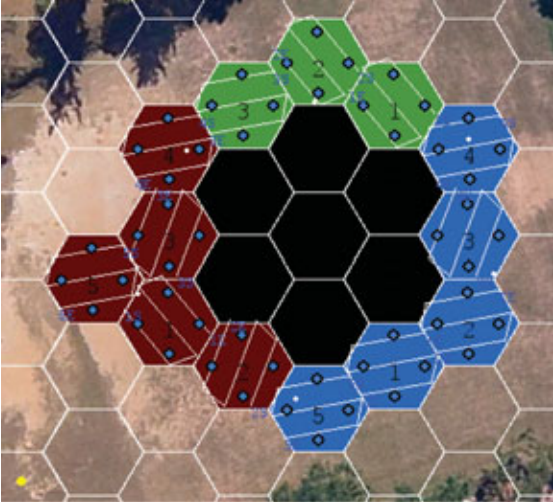
\includegraphics[scale=0.4]{figs/Hexagonal_Partitioning_Graphic}
	\caption{Simulation showing coverage of hexagonal partitions with back and forth motions with three robots. \cite{Azpurua2018}}
	\label{fig:Hex}
\end{figure}

\subsection{Voronoi Partitioning}
% Polygons
The individual path, to cover an area assigned to a robot, does not have to use simple motions. Often times, emphasis is placed on the area division algorithm and the single robot coverage paths are somewhat arbitrary. Those paths can be planned using any number of the single robot algorithms such as those mentioned in section \ref{sec:lit SR CPP}. In the mathematics field, there is work surrounding area division where they devise a method to divide a polygon into equal area polygons of a certain amount \cite{Nandakumar2012}. An old, but relevant, method that also stems from the field of mathematics, is the Voronoi partition. This assigns regions within an area to seeds based on distance. The idea is that a region assigned to a seed represents all the points where the distance to that seed is shorter than to any other seed.

% Voronoi
If the Voronoi partition is applied to the MCPP problem, the seeds once again become synonymous with robots. This partition works for any number of robots at any starting positions, but unless they are evenly spaced, the areas will all have varying sizes. Distances in these scenarios are usually Euclidean and the boundaries between areas represent the position where the distances from two seeds are equal. The authors of \cite{Nair2020} implement MCPP using Voronoi partitions in discrete space with static obstacles. They used square discretisation of the area and compared several different methods. They investigated geodesic-Manhattan-, Manhattan-, geodesic- and Euclidean-distance-based Voronoi partitions. 
% TODO: EDITING - Euclidean and Manhattan should always be with a capital letter 

Due to obstacles in the area, the Euclidean-based technique resulted in what the authors term "non-contiguous subregions". This means that the cells of a subregion are disconnected by an obstacle and cannot be covered completely by a single robot. They solve this problem by using geodesic distance. This uses Euclidean measurements, but instead of a straight line distance between two cells, it calculates the distance using a collision free path between the two cells. This kind of distance can be found using something like the A* point-to-point path planning algorithm.

Another problem arises, due to their use of discrete space. This was that when using Euclidean distances, some cells were partially in two subregions instead of fully in one or the other. Their solution was to use Manhattan distances, and ultimately the claim to have solved these problems by using geodisic-Manhattan-based distances to generate the partition. And thus they coined the term Geodesic-Manhattan Voronoi-Partition-Based Coverage (GM-VPC).

They implemented two different versions of GM-VPC, which utilize respectively an exact and an approximate individual area search technique. They implemented a boustrophedon coverage plan for the exact solution and a spanning tree for the approximate version. Both of these performed better when using geodesic-Manhattan distances.   

\begin{figure}[h!]
	\centering
	\begin{subfigure}[b]{0.45\textwidth}
		\centering
		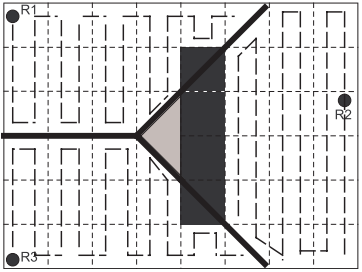
\includegraphics[scale=0.4]{figs/Voronoi_Euclid_BCD}
		\caption{Fig1}
		\label{fig:Voronoi - EuclidBCD}
	\end{subfigure}
	\hfill
	\begin{subfigure}[b]{0.45\textwidth}
		\centering
		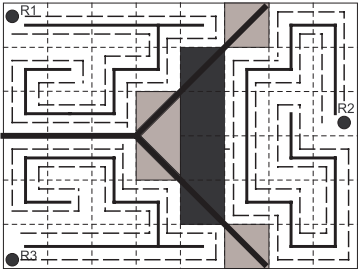
\includegraphics[scale=0.4]{figs/Voronoi_Euclid_STC}
		\caption{Fig2}
		\label{fig:Voronoi - EuclidSTC}
	\end{subfigure}
\caption{}
\end{figure}

\subsection{Negotiation Protocol}
A negotiation or bargaining protocol refers to a process involving task partitioning. In the context of area division for CPP, the task represents the area to be divided\cite{Rossi2009}. The authors of \cite{Rossi2009} present a negotiation model based on Rubinstein's alternate-offers protocol, for the purpose of area division. The focus of their implementation was to develop a distributed algorithm capable of considering robot capabilities. This means that the robots wouldn't have to be homogeneous and can have different flight-time capabilities, maneuverability, on-board equipment and so forth \cite{Barrientos2011}. 

They implemented their algorithm and found that it can achieve near optimum results. It tries to maximise the size of each robot's subdivision of the area (based on its capabilities), while also minimising sub-area overlap. The algorithm also works to avoid static obstacles or no fly zones that are present in the area. Moreover, they proved that it could be applied in a situation where re-planning may be necessary.
% Re-planning is necessary in a scenario when carrying out the plan changes the environment, thereby requireing replanning wiht the new environment scenario
% TODO: Future work - as new information about target becomes available - replan

A more complete implementation of the algorithm including an individual area search technique was also developed and tested \cite{Barrientos2011}. In this implementation they use a wavefront planner for the individual area coverage path generation. This requires discretisation of the area into cells. In their case, they used rectangles whose size was determined by on-board camera field of view (FOV). In order for the polygons generated by the negotiation protocol to work effectively, they use a method called Bresenham's line algorithm to approximate the lines that divide the areas in discrete space, so that they pass through the centroids of cells.

The area division achieved sometimes produces non-convex shapes, which the wavefront planner can handle effectively. Their implementation also minimizes energy consumption by minimizing the number of turns and not allowing backtracking. They also have the ability to specify the initial take-off positions of the robots. Distance from the specified take-off point to the starting point for sub-area coverage are considered in the sub-task negotiations. The authors also mention being able to specify robot landing positions preemptively.

One visible drawback in their implementation is that they coverage appears incomplete. The boundaries between areas pass through waypoints (cell centroids), that effectively get excluded from the coverage algorithm and are not covered. Using an exact method to search the individual areas could produce better results. Changing the boundaries to lie on the edges of cells rather than passing through their centroids could also make a difference.

\subsection{MSTC and MFC} 
Multi-robot spanning-tree coverage (MSTC) is a variant of single robot spanning tree coverage (STC) as presented in section \ref{sec:lit SR CPP - STC}. The authors of \cite{Hazon2005} designed the first variants of MSTC. The two variations they suggest are one that allows for backtracking and one that does not. Both variations still utilize a single spanning tree, but simply circumnavigate the tree with multiple robots instead of a single one.

They place a lot of emphasis on robustness and efficiency, in addition to completeness. They demonstrate an algorithm that segments the path around a spanning tree to evenly distribute it among robots. This distribution of robots is however, unrealistic. Their method becomes incredibly inefficient when robots are clustered closely together. This is because a robot simply navigates the path until it reaches the initial position of the next robot on the path. Figure \ref{fig:MSTC} shows the paths that are generated when the robots are evenly distributed along the path that circumnavigates the tree. Blue dots represent the robot initial positions and the spanning tree is shown in red. The second method they suggest remedies this somewhat. It allows for backtracking and improves the efficiency; which implies decreasing the time to completion.

The ideal situation is that all the robots have near equal path lengths, provided they are homogeneous robots. This is not guaranteed with this algorithm when the robots have random starting positions, but allowing for backtracking can improve the results and allow the coverage to be completed in a shorter amount of time. 

\begin{figure}
	\centering
	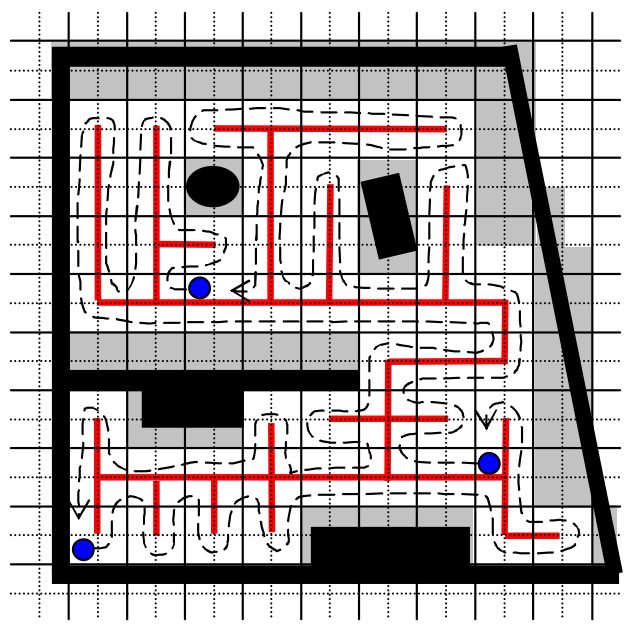
\includegraphics[scale=0.4]{figs/MSTC-Graphic}
	\caption{MSTC algorithm showing the paths for three robots on an environment grid. \cite{Hazon2005}}
	\label{fig:MSTC}
\end{figure}

\subsection{DARP}

%%%%%%%%%%%%%%%%%%%%%%%%%%%%%%%%%%%%%%%%%%%%%%%%%%%%%%%%%%%%%%%%%%%%%%%
\section{Non-Distributed Offline MCPP}
\subsection{Sampling-Based}
% Check Lavalle
\subsection{Artificial-Intelligence-Based}

%%%%%%%%%%%%%%%%%%%%%%%%%%%%%%%%%%%%%%%%%%%%%%%%%%%%%%%%%%%%%%%%%%%%%%%
\section{Online MCPP}

%%%%%%%%%%%%%%%%%%%%%%%%%%%%%%%%%%%%%%%%%%%%%%%%%%%%%%%%%%%%%%%%%%%%%%%

\section{UAVs and Search and Rescue}
%DroneSAR
%Rotary Wing vs Fixed-Wing UAVs}



\chapter{Environment Representation}
\label{chp:ER}
This section covers the environment representation. 
% TODO: Finish the preamble
%%%%%%%%%%%%%%%%%%%%%%%%%%%%%%%%%%%%%%%%%%%%%%%%%%%%%%%%%%%%%%%%%%%%%%%
\section{Background}
% TODO: Maybe divide this section into Scenario Description and then Background.
% TODO: Justify why you chose offline
% TODO: Justify why the target is not assumed to be in motion
The goal of this paper is to develop a coverage path planning algorithm \hbox{applicable} in a \acl{sar} situation. It should be implementable using \acsp{uav}, which can execute three dimensional movements. In this paper however, it is assumed that altitude changes are not necessary to search an area. Assuming that there is some form of camera on-board the \acs{uav}, a constant altitude will be an advantage. It means that the \acf{gsd} will remain constant, which is a widely accepted measure of camera accuracy. Assuming a camera is on a \acs{uav} pointing down towards the ground, \acs{gsd} is the distance on the ground as represented by the width of one pixel \cite{PropellerAero2021}.\\
Without altitude changes, \acs{uav} motions can be represented in two-dimensional space, which greatly simplifies the problem. For coverage path planning, it is important to have some demarcated two-dimensional region that requires coverage. The identified region, or environment, needs to be represented in either a discrete or continuous manner. \\
In the context of \acs{sar}, complete coverage is very important. It will ensure that every possible point in the environment map is covered. In this scenario, it implies that the camera will have viewed all points on the map. Achieving completeness is by no means trivial, but is more achievable in complex environments when using a discrete approach. \\
% TODO: Mention drawbacks of continuous implementations
% TODO: Mention reasons for choosing discrete - wavefront planner paper pg 674 "An exact cell decomposition is ineffiecient because we are interested in acquiring an equally sized set of images"
Discretising the environment can be done in a few different ways. Assuming a generic \acs{uav} with some thermal or visual camera on-board, one has a few options. One can discretise the area based on the \acs{uav} size, but a more common practice is to base it off the tool size. In this case, that would be the \acf{fov} of the on-board camera. This also makes the process of complete coverage easier, because if the camera is guaranteed to see the entirety of each discrete cell, it is a complete algorithm so long as each cell is visited.\\
Therefore, to discretise the environment, the \acl{fov} needs to be calculated. The camera specifications and \acs{uav} altitude will be the determining factors to calculate the \acs{fov}. The type of camera and the flight altitude are design decisions and will depend on the \acs{gsd} necessary to realistically be able to locate the target in a \acl{sar} operation.\\
The diagram in Figure \ref{fig:FOV} shows all the relevant variables needed to calculate the \acl{fov} along one dimension ($FOV_x$). A similar diagram can be used to calculate the \acl{fov} along the other dimension ($FOV_y$). The only difference would be the sensor size variable, which changes from the sensor width ($w_{len}$) to the sensor height ($h_{len}$). The other variables include the focal length of the camera ($f$), the height of the lens above ground ($H$) and the camera's angle of view ($AOV$). Lastly, there is the variable $\phi$ which is an angle created due to the sensor being slightly smaller than the diameter of the cone of light projected onto it.\\
The resulting \acl{fov} will be a rectangle of the same aspect ratio of the camera sensor, provided the camera is pointing directly down and the ground is level. For this application, it is assumed the camera is always pointing downwards. This can be accomplished when the \acs{uav} banks by placing the camera on a gimble. The assumption that the ground is level is not entirely reasonable, for example, in a mountainous region. This can be addressed by adding overlap between images to add some redundant coverage, which will be added in Chapter \ref{chp:refuelling}. Doing a topographical inspection is beyond the scope of this project and will not be addressed in more detail.\\
% TODO: Check this reference and decide whether to include last sentence
\tikzset{every picture/.style={line width=0.75pt}} %set default line width to 0.75pt          
\begin{figure}[h!]
	\centering	      
	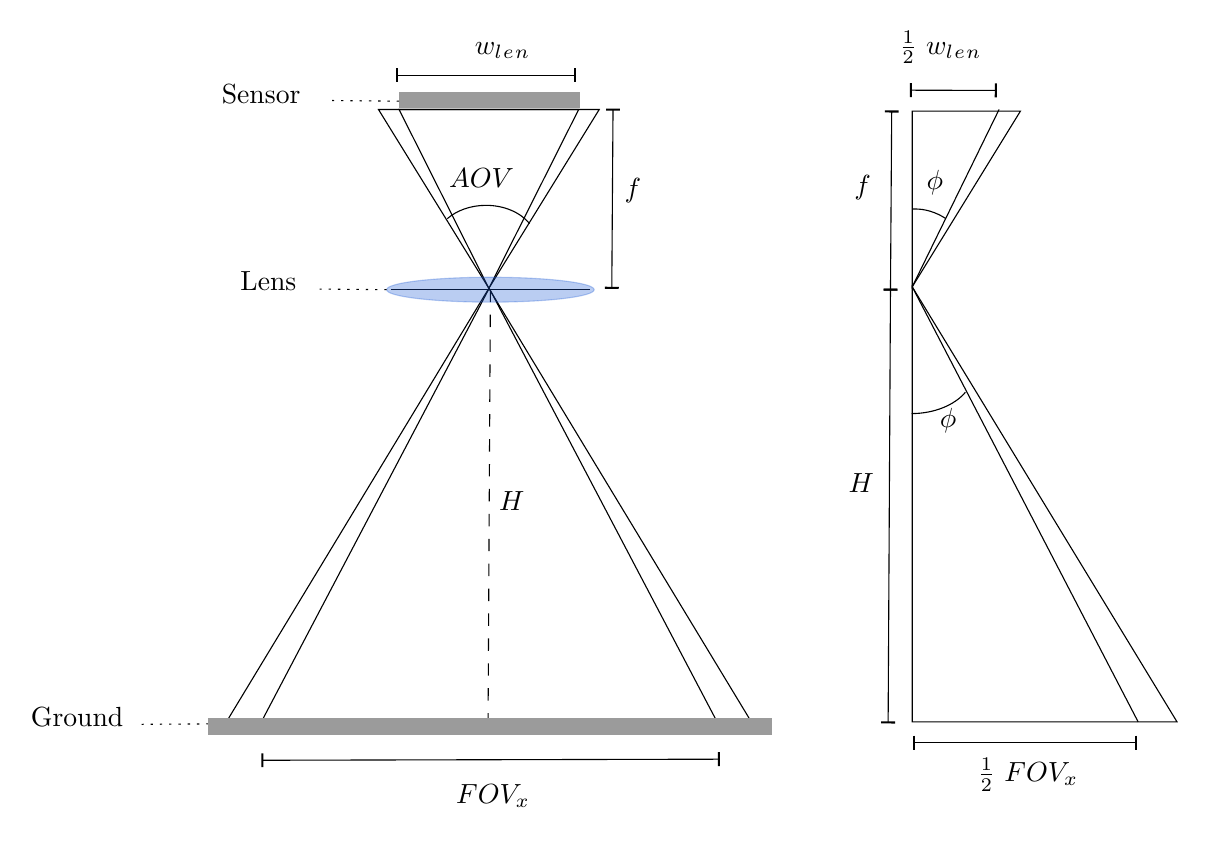
\begin{tikzpicture}[x=0.75pt,y=0.75pt,yscale=-1,xscale=1]
		%uncomment if require: \path (0,445); %set diagram left start at 0, and has height of 445
		
		%Shape: Triangle [id:dp7279031821934365] 
		\draw   (292.52,162.29) -- (239.35,76.17) -- (345.69,76.17) -- cycle ;
		%Shape: Triangle [id:dp08500924272014787] 
		\draw   (292.52,162.29) -- (419.57,372.17) -- (165.48,372.17) -- cycle ;
		%Straight Lines [id:da9387157545116658] 
		\draw    (245.26,162.97) -- (341.26,162.97) ;
		%Shape: Triangle [id:dp15441481766796317] 
		\draw   (292.52,162.29) -- (249.26,76.17) -- (335.78,76.17) -- cycle ;
		%Shape: Triangle [id:dp8187279481172025] 
		\draw   (292.69,162.29) -- (403,372.17) -- (182.39,372.17) -- cycle ;
		%Straight Lines [id:da06491692932377724] 
		\draw    (248.39,59.69) -- (334.14,59.69) ;
		\draw [shift={(334.14,59.69)}, rotate = 180] [color={rgb, 255:red, 0; green, 0; blue, 0 }  ][line width=0.75]    (0,3.35) -- (0,-3.35)   ;
		\draw [shift={(248.39,59.69)}, rotate = 180] [color={rgb, 255:red, 0; green, 0; blue, 0 }  ][line width=0.75]    (0,3.35) -- (0,-3.35)   ;
		%Straight Lines [id:da8254572040663344] 
		\draw    (352.34,76.22) -- (351.75,162.07) ;
		\draw [shift={(351.75,162.07)}, rotate = 270.39] [color={rgb, 255:red, 0; green, 0; blue, 0 }  ][line width=0.75]    (0,3.35) -- (0,-3.35)   ;
		\draw [shift={(352.34,76.22)}, rotate = 270.39] [color={rgb, 255:red, 0; green, 0; blue, 0 }  ][line width=0.75]    (0,3.35) -- (0,-3.35)   ;
		%Straight Lines [id:da18153445552160163] 
		\draw  [dash pattern={on 4.5pt off 4.5pt}]  (293.26,162.97) -- (292.13,371.48) ;
		%Shape: Right Triangle [id:dp9464990257102419] 
		\draw   (548.64,76.92) -- (496.5,161.6) -- (496.5,76.94) -- cycle ;
		%Straight Lines [id:da9593228177444686] 
		\draw    (496.5,161.6) -- (538.33,76.17) ;
		%Shape: Arc [id:dp3427993390498929] 
		\draw  [draw opacity=0] (496.65,124.11) .. controls (496.93,124.1) and (497.22,124.09) .. (497.5,124.09) .. controls (502.76,124) and (507.83,125.61) .. (512.56,128.62) -- (498.77,204.83) -- cycle ; \draw   (496.65,124.11) .. controls (496.93,124.1) and (497.22,124.09) .. (497.5,124.09) .. controls (502.76,124) and (507.83,125.61) .. (512.56,128.62) ;
		%Straight Lines [id:da5534147172451449] 
		\draw    (495.86,66.85) -- (536.76,66.97) ;
		\draw [shift={(536.76,66.97)}, rotate = 180.17] [color={rgb, 255:red, 0; green, 0; blue, 0 }  ][line width=0.75]    (0,3.35) -- (0,-3.35)   ;
		\draw [shift={(495.86,66.85)}, rotate = 180.17] [color={rgb, 255:red, 0; green, 0; blue, 0 }  ][line width=0.75]    (0,3.35) -- (0,-3.35)   ;
		%Straight Lines [id:da49349314045709525] 
		\draw    (486.61,77.11) -- (486.02,162.96) ;
		\draw [shift={(486.02,162.96)}, rotate = 270.39] [color={rgb, 255:red, 0; green, 0; blue, 0 }  ][line width=0.75]    (0,3.35) -- (0,-3.35)   ;
		\draw [shift={(486.61,77.11)}, rotate = 270.39] [color={rgb, 255:red, 0; green, 0; blue, 0 }  ][line width=0.75]    (0,3.35) -- (0,-3.35)   ;
		%Shape: Arc [id:dp09088039941092019] 
		\draw  [draw opacity=0] (272.52,128.74) .. controls (277.02,124.82) and (283.7,122.33) .. (291.17,122.33) .. controls (300.03,122.33) and (307.8,125.84) .. (312.1,131.09) -- (291.17,140.58) -- cycle ; \draw   (272.52,128.74) .. controls (277.02,124.82) and (283.7,122.33) .. (291.17,122.33) .. controls (300.03,122.33) and (307.8,125.84) .. (312.1,131.09) ;
		%Shape: Right Triangle [id:dp9191394953697831] 
		\draw   (496.5,161.6) -- (624.06,371.17) -- (496.5,371.17) -- cycle ;
		%Straight Lines [id:da9606752421348479] 
		\draw    (605.33,371.17) -- (496.5,161.6) ;
		%Shape: Arc [id:dp6813474716985082] 
		\draw  [draw opacity=0] (522.1,212.41) .. controls (516.97,218.5) and (507.3,222.62) .. (496.19,222.67) -- (496,202.42) -- cycle ; \draw   (522.1,212.41) .. controls (516.97,218.5) and (507.3,222.62) .. (496.19,222.67) ;
		%Straight Lines [id:da806740169220673] 
		\draw    (183.39,389.69) -- (403.33,389.17) ;
		\draw [shift={(403.33,389.17)}, rotate = 539.86] [color={rgb, 255:red, 0; green, 0; blue, 0 }  ][line width=0.75]    (0,3.35) -- (0,-3.35)   ;
		\draw [shift={(183.39,389.69)}, rotate = 539.86] [color={rgb, 255:red, 0; green, 0; blue, 0 }  ][line width=0.75]    (0,3.35) -- (0,-3.35)   ;
		%Straight Lines [id:da8133225602503578] 
		\draw    (497.33,381.17) -- (604.33,381.17) ;
		\draw [shift={(604.33,381.17)}, rotate = 180] [color={rgb, 255:red, 0; green, 0; blue, 0 }  ][line width=0.75]    (0,3.35) -- (0,-3.35)   ;
		\draw [shift={(497.33,381.17)}, rotate = 180] [color={rgb, 255:red, 0; green, 0; blue, 0 }  ][line width=0.75]    (0,3.35) -- (0,-3.35)   ;
		%Straight Lines [id:da25053349814928394] 
		\draw    (486.02,162.96) -- (484.89,371.47) ;
		\draw [shift={(484.89,371.47)}, rotate = 270.31] [color={rgb, 255:red, 0; green, 0; blue, 0 }  ][line width=0.75]    (0,3.35) -- (0,-3.35)   ;
		\draw [shift={(486.02,162.96)}, rotate = 270.31] [color={rgb, 255:red, 0; green, 0; blue, 0 }  ][line width=0.75]    (0,3.35) -- (0,-3.35)   ;
		%Shape: Rectangle [id:dp5196090784877698] 
		\draw  [color={rgb, 255:red, 155; green, 155; blue, 155 }  ,draw opacity=1 ][fill={rgb, 255:red, 155; green, 155; blue, 155 }  ,fill opacity=1 ] (249.26,68.14) -- (336,68.14) -- (336,75.17) -- (249.26,75.17) -- cycle ;
		%Shape: Ellipse [id:dp39537204861922115] 
		\draw  [color={rgb, 255:red, 26; green, 88; blue, 211 }  ,draw opacity=0.3 ][fill={rgb, 255:red, 26; green, 88; blue, 211 }  ,fill opacity=0.3 ] (243.26,162.97) .. controls (243.26,159.66) and (265.64,156.97) .. (293.26,156.97) .. controls (320.87,156.97) and (343.26,159.66) .. (343.26,162.97) .. controls (343.26,166.29) and (320.87,168.97) .. (293.26,168.97) .. controls (265.64,168.97) and (243.26,166.29) .. (243.26,162.97) -- cycle ;
		%Shape: Boxed Line [id:dp7067135001640237] 
		\draw  [dash pattern={on 0.84pt off 2.51pt}]  (243.26,162.97) -- (211,162.67) ;
		%Straight Lines [id:da962687715126145] 
		\draw  [dash pattern={on 0.84pt off 2.51pt}]  (157.48,372.17) -- (125.22,372.37) ;
		%Shape: Boxed Line [id:dp25644897900816477] 
		\draw  [dash pattern={on 0.84pt off 2.51pt}]  (249.26,72.14) -- (217,71.84) ;
		%Straight Lines [id:da9121328450253205] 
		\draw [color={rgb, 255:red, 155; green, 155; blue, 155 }  ,draw opacity=1 ][line width=6]    (157.17,373.35) -- (429.09,373.35) ;
		
		% Text Node
		\draw (277.85,37.29) node [anchor=north west][inner sep=0.75pt]  [font=\normalsize]  {$ \begin{array}{l}
				w_{l}{}_{e}{}_{n}\\
			\end{array}$};
		% Text Node
		\draw (171.59,152.9) node [anchor=north west][inner sep=0.75pt]  [font=\normalsize] [align=left] {Lens};
		% Text Node
		\draw (356.67,108.27) node [anchor=north west][inner sep=0.75pt]  [font=\normalsize]  {$f$};
		% Text Node
		\draw (296.25,259.08) node [anchor=north west][inner sep=0.75pt]  [font=\normalsize]  {$H$};
		% Text Node
		\draw (272.06,103.36) node [anchor=north west][inner sep=0.75pt]  [font=\normalsize]  {$AOV$};
		% Text Node
		\draw (502.19,104.3) node [anchor=north west][inner sep=0.75pt]  [font=\normalsize]  {$\phi $};
		% Text Node
		\draw (467.33,106.6) node [anchor=north west][inner sep=0.75pt]  [font=\normalsize]  {$f$};
		% Text Node
		\draw (489,37) node [anchor=north west][inner sep=0.75pt]    {$\frac{1}{2} \ w_{l}{}_{e}{}_{n}$};
		% Text Node
		\draw (508.52,218.96) node [anchor=north west][inner sep=0.75pt]  [font=\normalsize]  {$\phi $};
		% Text Node
		\draw (268.85,398.07) node [anchor=north west][inner sep=0.75pt]  [font=\normalsize]  {$ \begin{array}{l}
				FOV_{x}\\
			\end{array}$};
		% Text Node
		\draw (520,387.4) node [anchor=north west][inner sep=0.75pt]  [font=\normalsize]  {$ \begin{array}{l}
				\frac{1}{2} \ FOV_{x}\\
			\end{array}$};
		% Text Node
		\draw (464.59,250.41) node [anchor=north west][inner sep=0.75pt]  [font=\normalsize]  {$H$};
		% Text Node
		\draw (162.59,62.9) node [anchor=north west][inner sep=0.75pt]  [font=\normalsize] [align=left] {Sensor};
		% Text Node
		\draw (70.59,363) node [anchor=north west][inner sep=0.75pt]  [font=\normalsize] [align=left] {Ground};
		
		
	\end{tikzpicture}
	\caption{Diagram showing relevant variables concerned with calculating the Field of View for a camera.}
	\label{fig:FOV}
\end{figure}
The calculations required to do a discretisation based on the camera \acl{fov} will now be discussed. The first equation that is required is the calculation of the angle $\phi$ which makes use of the small triangle:
\begin{equation}
	\label{eqn:phi}
	\begin{aligned}
		\tan{\phi} &= \frac{\frac{1}{2}w_{len}}{f} &\\
		\phi &= \tan^{-1}{(\frac{w_{len}}{2f})}
	\end{aligned}	
\end{equation}
Now that $\phi$ is known, the bigger triangle is used to calculate $FOV_x$:
\begin{equation}
	\label{eqn:fov_x}
	\begin{aligned}
		\frac{FOV_x}{2} &= H \times \tan{\phi} &\\
		FOV_x &= 2H \times \tan{ (\tan^{-1}{ (\frac{w_{len}}{2f}) }) } &\\
		FOV_x &= H \times \frac{w_{len}}{f} &\\
	\end{aligned}
\end{equation}
Similarly, $FOV_y$ can be calculated using the other sensor size dimension $h_{len}$:
\begin{equation}
	\label{eqn:fov_y}
	\begin{aligned}
		FOV_y &= H \times \frac{h_{len}}{f}
	\end{aligned}
\end{equation}
Both $FOV_x$ and $FOV_y$ will have the same units as $H$, which is metres. The resolution of the camera is the number of pixels along the image width ($px_w$) multiplied with the number of pixels along its height ($px_h$). These can be used to calculate the $GSD$ by dividing either $FOV$ by the pixel value associated with that dimension:
\begin{equation}
	\label{eqn:GSD}
	\begin{aligned}
		GSD &= \frac{100FOV_x}{px_w} &\\
		GSD &= \frac{100H \times w_{len}}{f \times px_w}
	\end{aligned}
\end{equation}

\section{Environment Discretisation}
If the size of the environment discretisation is set equal to the rectangular camera field of view, and the type of camera used is known, then a desired $GSD$ can be used to decide on an appropriate flying height. Choosing a $GSD$ would depend on the application, seen as it represents the level of detail that can potentially be detected in an image.\\
Taking the conservative approach, the assumption is that one is looking for a human being standing upright, viewed from above. To get a good estimate of the space occupied by a human in this orientation, one needs anthropometric data. A survey was done in Europe for people between the ages of 18 and 60 \cite{Jurgens1998}. Among other measurements, they measured chest depth ($w$) and elbow-to-elbow length ($l$). These dimensions represent those of an upright human from above and can be seen in Figure \ref{fig:GSD}.\\ 
\tikzset{every picture/.style={line width=0.75pt}} %set default line width to 0.75pt        
\begin{figure}
	\centering
	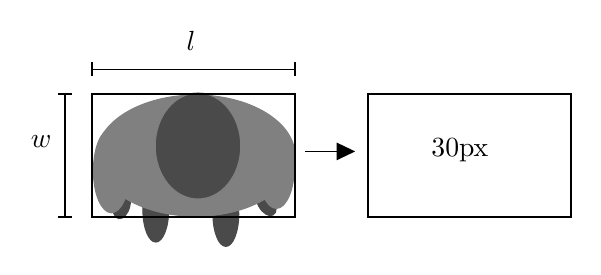
\begin{tikzpicture}[x=0.75pt,y=0.75pt,yscale=-1,xscale=1]
		%uncomment if require: \path (0,300); %set diagram left start at 0, and has height of 300
		
		%Shape: Ellipse [id:dp5061908839346234] 
		\draw  [color={rgb, 255:red, 74; green, 74; blue, 74 }  ,draw opacity=1 ][fill={rgb, 255:red, 74; green, 74; blue, 74 }  ,fill opacity=1 ] (394.62,193.23) .. controls (392.81,189.9) and (392.91,186.34) .. (394.85,185.28) .. controls (396.79,184.23) and (399.83,186.07) .. (401.65,189.41) .. controls (403.47,192.74) and (403.37,196.3) .. (401.43,197.36) .. controls (399.49,198.41) and (396.44,196.57) .. (394.62,193.23) -- cycle ;
		%Shape: Ellipse [id:dp4772697686098053] 
		\draw  [color={rgb, 255:red, 74; green, 74; blue, 74 }  ,draw opacity=1 ][fill={rgb, 255:red, 74; green, 74; blue, 74 }  ,fill opacity=1 ] (324.6,191.47) .. controls (325.46,187.77) and (327.9,185.18) .. (330.05,185.68) .. controls (332.2,186.18) and (333.25,189.58) .. (332.4,193.28) .. controls (331.54,196.98) and (329.1,199.57) .. (326.95,199.07) .. controls (324.8,198.57) and (323.75,195.17) .. (324.6,191.47) -- cycle ;
		%Shape: Ellipse [id:dp7464833674207887] 
		\draw  [color={rgb, 255:red, 74; green, 74; blue, 74 }  ,draw opacity=1 ][fill={rgb, 255:red, 74; green, 74; blue, 74 }  ,fill opacity=1 ] (372.5,196.92) .. controls (372.5,188.32) and (375.28,181.35) .. (378.71,181.35) .. controls (382.13,181.35) and (384.91,188.32) .. (384.91,196.92) .. controls (384.91,205.53) and (382.13,212.5) .. (378.71,212.5) .. controls (375.28,212.5) and (372.5,205.53) .. (372.5,196.92) -- cycle ;
		%Shape: Ellipse [id:dp9681716059666354] 
		\draw  [color={rgb, 255:red, 74; green, 74; blue, 74 }  ,draw opacity=1 ][fill={rgb, 255:red, 74; green, 74; blue, 74 }  ,fill opacity=1 ] (338.74,194.85) .. controls (338.74,186.24) and (341.52,179.27) .. (344.95,179.27) .. controls (348.37,179.27) and (351.15,186.24) .. (351.15,194.85) .. controls (351.15,203.45) and (348.37,210.42) .. (344.95,210.42) .. controls (341.52,210.42) and (338.74,203.45) .. (338.74,194.85) -- cycle ;
		%Shape: Ellipse [id:dp7224271801321214] 
		\draw  [color={rgb, 255:red, 128; green, 128; blue, 128 }  ,draw opacity=1 ][fill={rgb, 255:red, 128; green, 128; blue, 128 }  ,fill opacity=1 ] (316.38,168.78) .. controls (316.38,152.66) and (337.79,139.6) .. (364.19,139.6) .. controls (390.59,139.6) and (412,152.66) .. (412,168.78) .. controls (412,184.9) and (390.59,197.96) .. (364.19,197.96) .. controls (337.79,197.96) and (316.38,184.9) .. (316.38,168.78) -- cycle ;
		%Shape: Ellipse [id:dp3950279689736771] 
		\draw  [color={rgb, 255:red, 128; green, 128; blue, 128 }  ,draw opacity=1 ][fill={rgb, 255:red, 74; green, 74; blue, 74 }  ,fill opacity=1 ] (365.29,138.6) .. controls (376.67,138.6) and (385.9,150.04) .. (385.9,164.15) .. controls (385.9,178.25) and (376.67,189.69) .. (365.29,189.69) .. controls (353.9,189.69) and (344.67,178.25) .. (344.67,164.15) .. controls (344.67,150.04) and (353.9,138.6) .. (365.29,138.6) -- cycle ;
		%Shape: Ellipse [id:dp14441581895383182] 
		\draw  [color={rgb, 255:red, 128; green, 128; blue, 128 }  ,draw opacity=1 ][fill={rgb, 255:red, 128; green, 128; blue, 128 }  ,fill opacity=1 ] (314.91,176.05) .. controls (314.91,164.87) and (318.8,155.8) .. (323.6,155.8) .. controls (328.4,155.8) and (332.29,164.87) .. (332.29,176.05) .. controls (332.29,187.23) and (328.4,196.3) .. (323.6,196.3) .. controls (318.8,196.3) and (314.91,187.23) .. (314.91,176.05) -- cycle ;
		%Shape: Ellipse [id:dp8509174208950578] 
		\draw  [color={rgb, 255:red, 128; green, 128; blue, 128 }  ,draw opacity=1 ][fill={rgb, 255:red, 128; green, 128; blue, 128 }  ,fill opacity=1 ] (394.35,173.97) .. controls (394.35,162.79) and (398.24,153.72) .. (403.03,153.72) .. controls (407.83,153.72) and (411.72,162.79) .. (411.72,173.97) .. controls (411.72,185.16) and (407.83,194.22) .. (403.03,194.22) .. controls (398.24,194.22) and (394.35,185.16) .. (394.35,173.97) -- cycle ;
		%Shape: Rectangle [id:dp6763821992887933] 
		\draw  [line width=0.75]  (314.19,139.1) -- (412.19,139.1) -- (412.19,198.46) -- (314.19,198.46) -- cycle ;
		%Straight Lines [id:da0050447787628182805] 
		\draw    (314.19,127.1) -- (412.19,127.1) ;
		\draw [shift={(412.19,127.1)}, rotate = 180] [color={rgb, 255:red, 0; green, 0; blue, 0 }  ][line width=0.75]    (0,3.35) -- (0,-3.35)   ;
		\draw [shift={(314.19,127.1)}, rotate = 180] [color={rgb, 255:red, 0; green, 0; blue, 0 }  ][line width=0.75]    (0,3.35) -- (0,-3.35)   ;
		%Shape: Rectangle [id:dp8520376009638861] 
		\draw  [line width=0.75]  (447.19,139.1) -- (545.19,139.1) -- (545.19,198.46) -- (447.19,198.46) -- cycle ;
		%Straight Lines [id:da004734927691815605] 
		\draw    (417,166.75) -- (438,166.75) ;
		\draw [shift={(441,166.75)}, rotate = 540] [fill={rgb, 255:red, 0; green, 0; blue, 0 }  ][line width=0.08]  [draw opacity=0] (8.93,-4.29) -- (0,0) -- (8.93,4.29) -- cycle    ;
		%Straight Lines [id:da5120965397340576] 
		\draw    (301.19,139.1) -- (301.19,198.46) ;
		\draw [shift={(301.19,198.46)}, rotate = 270] [color={rgb, 255:red, 0; green, 0; blue, 0 }  ][line width=0.75]    (0,3.35) -- (0,-3.35)   ;
		\draw [shift={(301.19,139.1)}, rotate = 270] [color={rgb, 255:red, 0; green, 0; blue, 0 }  ][line width=0.75]    (0,3.35) -- (0,-3.35)   ;
		
		% Text Node
		\draw (358.5,107.4) node [anchor=north west][inner sep=0.75pt]    {$l$};
		% Text Node
		\draw (283.5,157.9) node [anchor=north west][inner sep=0.75pt]    {$w$};
		% Text Node
		\draw (476.5,159.5) node [anchor=north west][inner sep=0.75pt]   [align=left] {30px};		
	\end{tikzpicture}
	\caption{Figure showing the rectangular approximation for a human viewed from above for calculation of the GSD}
	\label{fig:GSD}
\end{figure}
To calculate \acs{gsd}, a minimum number of pixels needed to make a human visible must be chosen. There is an article wherein they developed an image processing algorithm for human detection in a \acl{sar} scenario \cite{Rudol2008}. In this article they made the decision to put a 30 pixel requirement on human detection.
% TODO: Maybe refer back to the literature review where the Rudol paper should be mentioned for the first time.
Figure \ref{fig:GSD} shows the rectangular approximation for a human that the 30 pixels should represent.\\
Using the lower percentile measurements of 170mm chest depth and 390mm elbow-to-elbow length along with the 30 pixel requirement, one gets a \acs{gsd} of roughly 4.7cm/px. For a child, these values could be even smaller. Therefore, 4cm/px will be used to calculate an appropriate flying height, which is a reasonable value considering that most aerial surveys operate at a \acs{gsd} of less than 5cm/px \cite{PropellerAero2021}.\\
To show how the \acs{gsd} requirement can be used, a series of cameras are chosen to demonstrate how the discretisation could be determined using the camera specifications and the maximum allowable \acs{gsd}. Before showing the calculations applied to a specific scenario, they are shown in a more general sense. Firstly, one calculates the maximum allowable height:
\begin{equation}
	\label{eqn:height_calculation}
	\begin{aligned}
		H_{max} &= \frac{GSD_{max} \times f \times px_w}{100w_{len}}
	\end{aligned}
\end{equation}
It is desirable to fly as high as possible, because this decreases the coverage time by increasing the camera \acl{fov}. Therefore, the assumption is that the height chosen would be the maximum, provided this is within the capabilities of the \acs{uav}. Using Equations \ref{eqn:fov_x} and \ref{eqn:fov_y}, one can then calculate the camera \acs{fov} at the height chosen.\\
% discretisation - square vs rectangular
One can now discretise the environment based on this field of view. One option is to do a square discretisation. One would make the squares have sides equal to the smaller \acs{fov} dimension, which is $FOV_y$. An example of this discretisation can be seen in Figure \ref{fig:Overlap-sqr}. This technique will always have cross-track overlap. This means that there will be a percentage of redundant coverage. If a camera has a square \acs{fov} then the overlap goes away, but this is uncommon. They tend to have a 4:3 or 3:2 aspect ratio. There is the option of making the squares have side lengths equal to $FOV_x$, but then complete coverage would not be achievable by simply following the square centroids. This adds a layer of complexity unnecessarily. Setting the square side length equal to $l$, one can calculate the cross-track overlap using the following equation:
\begin{equation}
	\label{eqn:overlap_sqr}
	\begin{aligned}
		Provided&,& ~~l &\leq FOV_y& \\
		Then&,& ~~\%Overlap &= \frac{l(FOV_x - l)}{l^2} \times 100&
	\end{aligned}
\end{equation}
Figure \ref{fig:Overlap-rect} shows an alternative technique where the environment is divided into rectangles. With this there is no overlap when moving in the $y$ direction, but there is when moving in the $x$ direction. An environment would be covered faster with this technique provided the $y$ direction is favoured during flight, but no overlap in the $y$ direction is risky. In this scenario, the cross-track overlap over the span of one rectangle when moving in the $y$ direction is zero and for the $x$ direction it can be calculated as follows:
\begin{equation}
	\label{eqn:overlap_rect}
	\begin{aligned}
		\%Overlap &= \frac{FOV_x(FOV_x-FOV_y)}{FOV_x-FOV_y} \times 100&
	\end{aligned}
\end{equation}
Both techniques assume sharp 90 degree turns are possible. Some \acsp{uav} can make sharp turns, such as multi-rotors, but this often requires deceleration to a hover, which significantly slows coverage time by lowering the average velocity during coverage. Chapter \ref{chp:Dynamic} covers a proposed solution for a constant speed scenario. This is considerably more favourable in a scenario where a fixed-wing \acs{uav} is used instead of a multi-rotor. Fixed-wing craft are desirable for \acs{sar} due to there high endurance. They can generally cover larger areas before needing to refuel.\\
% TODO: check if you used chapter in all chapter references.
\begin{figure}[]
	\centering
	\begin{subfigure}[b]{0.45\textwidth}
		\centering
			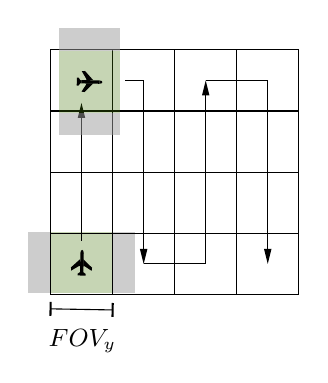
\begin{tikzpicture}[x=0.75pt,y=0.75pt,yscale=-1,xscale=1]
			%uncomment if require: \path (0,300); %set diagram left start at 0, and has height of 300
			
			%Shape: Rectangle [id:dp036802263347778474] 
			\draw  [draw opacity=0][fill={rgb, 255:red, 65; green, 117; blue, 5 }  ,fill opacity=0.3 ] (91.4,162.11) -- (121.3,162.11) -- (121.3,191.57) -- (91.4,191.57) -- cycle ;
			%Shape: Chord [id:dp8311663081836851] 
			\draw  [draw opacity=0][fill={rgb, 255:red, 0; green, 0; blue, 0 }  ,fill opacity=1 ] (105.79,172.1) .. controls (105.79,172.1) and (105.79,172.1) .. (105.79,172.1) .. controls (105.8,171.29) and (106.18,170.63) .. (106.62,170.64) .. controls (107.06,170.66) and (107.41,171.32) .. (107.39,172.14) -- cycle ;
			%Shape: Rectangle [id:dp8012179965756234] 
			\draw  [draw opacity=0][fill={rgb, 255:red, 0; green, 0; blue, 0 }  ,fill opacity=1 ] (107.39,172.14) -- (107.23,180.82) -- (105.62,180.78) -- (105.78,172.1) -- cycle ;
			%Shape: Chord [id:dp46276085808629674] 
			\draw  [draw opacity=0][fill={rgb, 255:red, 0; green, 0; blue, 0 }  ,fill opacity=1 ] (107.23,180.82) .. controls (107.23,180.82) and (107.23,180.82) .. (107.23,180.82) .. controls (107.21,181.63) and (106.84,182.28) .. (106.4,182.27) .. controls (105.95,182.26) and (105.61,181.59) .. (105.62,180.78) -- cycle ;
			%Shape: Boxed Polygon [id:dp33577441359912386] 
			\draw  [draw opacity=0][fill={rgb, 255:red, 0; green, 0; blue, 0 }  ,fill opacity=1 ] (111.19,180.75) -- (107.86,178.55) -- (107.16,178.35) -- (107.21,175.15) -- (111.37,179.23) -- cycle ;
			%Shape: Boxed Polygon [id:dp4613372486056908] 
			\draw  [draw opacity=0][fill={rgb, 255:red, 0; green, 0; blue, 0 }  ,fill opacity=1 ] (101.36,180.59) -- (104.88,178.52) -- (105.61,178.35) -- (105.65,175.11) -- (101.22,179.05) -- cycle ;
			%Shape: Boxed Polygon [id:dp09882619727387199] 
			\draw  [draw opacity=0][fill={rgb, 255:red, 0; green, 0; blue, 0 }  ,fill opacity=1 ] (108.27,182.2) -- (108.23,183.06) -- (104.44,182.93) -- (104.47,182.1) -- (106.42,180.8) -- cycle ;
			
			%Shape: Rectangle [id:dp43518650932458014] 
			\draw  [draw opacity=0][fill={rgb, 255:red, 155; green, 155; blue, 155 }  ,fill opacity=0.5 ] (121.3,162.07) -- (132.06,162.07) -- (132.06,191.61) -- (121.3,191.61) -- cycle ;
			%Shape: Rectangle [id:dp898186670672066] 
			\draw  [draw opacity=0][fill={rgb, 255:red, 155; green, 155; blue, 155 }  ,fill opacity=0.5 ] (80.64,162.07) -- (91.4,162.07) -- (91.4,191.61) -- (80.64,191.61) -- cycle ;
			
			%Shape: Rectangle [id:dp12911688161174095] 
			\draw   (91.4,74.26) -- (121.3,74.26) -- (121.3,103.72) -- (91.4,103.72) -- cycle ;
			%Shape: Rectangle [id:dp778307202398685] 
			\draw   (121.3,74.26) -- (151.2,74.26) -- (151.2,103.72) -- (121.3,103.72) -- cycle ;
			%Shape: Rectangle [id:dp5920975737411569] 
			\draw   (151.2,74.26) -- (181.1,74.26) -- (181.1,103.72) -- (151.2,103.72) -- cycle ;
			%Shape: Rectangle [id:dp7108929033014086] 
			\draw   (91.4,103.72) -- (121.3,103.72) -- (121.3,133.18) -- (91.4,133.18) -- cycle ;
			%Shape: Rectangle [id:dp8152064023887235] 
			\draw   (91.4,133.18) -- (121.3,133.18) -- (121.3,162.64) -- (91.4,162.64) -- cycle ;
			%Shape: Rectangle [id:dp01596026185419297] 
			\draw   (181.1,162.64) -- (211,162.64) -- (211,192.11) -- (181.1,192.11) -- cycle ;
			%Shape: Rectangle [id:dp7327882569457931] 
			\draw   (121.3,103.72) -- (151.2,103.72) -- (151.2,133.18) -- (121.3,133.18) -- cycle ;
			%Shape: Rectangle [id:dp11348064360337196] 
			\draw   (121.3,133.18) -- (151.2,133.18) -- (151.2,162.64) -- (121.3,162.64) -- cycle ;
			%Shape: Rectangle [id:dp5274571336670886] 
			\draw   (151.2,133.18) -- (181.1,133.18) -- (181.1,162.64) -- (151.2,162.64) -- cycle ;
			%Shape: Rectangle [id:dp1361244585482333] 
			\draw   (151.2,103.72) -- (181.1,103.72) -- (181.1,133.18) -- (151.2,133.18) -- cycle ;
			%Shape: Rectangle [id:dp8698952772815938] 
			\draw   (91.4,162.64) -- (121.3,162.64) -- (121.3,192.11) -- (91.4,192.11) -- cycle ;
			%Shape: Rectangle [id:dp8275138362077274] 
			\draw   (121.3,162.64) -- (151.2,162.64) -- (151.2,192.11) -- (121.3,192.11) -- cycle ;
			%Shape: Rectangle [id:dp5045016465037775] 
			\draw   (151.2,162.64) -- (181.1,162.64) -- (181.1,192.11) -- (151.2,192.11) -- cycle ;
			%Shape: Rectangle [id:dp5051198991702088] 
			\draw   (181.1,133.18) -- (211,133.18) -- (211,162.64) -- (181.1,162.64) -- cycle ;
			%Shape: Rectangle [id:dp9607013415516779] 
			\draw   (181.1,103.72) -- (211,103.72) -- (211,133.18) -- (181.1,133.18) -- cycle ;
			%Shape: Rectangle [id:dp5794670437040133] 
			\draw   (181.1,74.26) -- (211,74.26) -- (211,103.72) -- (181.1,103.72) -- cycle ;
			%Straight Lines [id:da9321367214575229] 
			\draw    (106.29,166.14) -- (106.29,101.86) ;
			\draw [shift={(106.29,99.86)}, rotate = 450] [fill={rgb, 255:red, 0; green, 0; blue, 0 }  ][line width=0.08]  [draw opacity=0] (7.2,-1.8) -- (0,0) -- (7.2,1.8) -- cycle    ;
			%Straight Lines [id:da40799678234401227] 
			\draw    (166.15,177.38) -- (166.15,90.99) ;
			\draw [shift={(166.15,88.99)}, rotate = 450] [fill={rgb, 255:red, 0; green, 0; blue, 0 }  ][line width=0.08]  [draw opacity=0] (7.2,-1.8) -- (0,0) -- (7.2,1.8) -- cycle    ;
			%Straight Lines [id:da2047551510485104] 
			\draw    (136.25,89.23) -- (127.29,89.23) ;
			%Shape: Rectangle [id:dp8051835391549806] 
			\draw  [draw opacity=0][fill={rgb, 255:red, 65; green, 117; blue, 5 }  ,fill opacity=0.3 ] (124.94,74.61) -- (124.94,104.51) -- (95.48,104.51) -- (95.48,74.61) -- cycle ;
			%Shape: Chord [id:dp01440978675599247] 
			\draw  [draw opacity=0][fill={rgb, 255:red, 0; green, 0; blue, 0 }  ,fill opacity=1 ] (114.95,88.99) .. controls (114.95,88.99) and (114.95,88.99) .. (114.95,88.99) .. controls (115.76,89.01) and (116.42,89.38) .. (116.4,89.83) .. controls (116.39,90.27) and (115.72,90.61) .. (114.91,90.6) -- cycle ;
			%Shape: Rectangle [id:dp47820815125081073] 
			\draw  [draw opacity=0][fill={rgb, 255:red, 0; green, 0; blue, 0 }  ,fill opacity=1 ] (114.91,90.6) -- (106.23,90.43) -- (106.27,88.82) -- (114.95,88.99) -- cycle ;
			%Shape: Chord [id:dp5606590464537962] 
			\draw  [draw opacity=0][fill={rgb, 255:red, 0; green, 0; blue, 0 }  ,fill opacity=1 ] (106.23,90.43) .. controls (105.42,90.42) and (104.77,90.05) .. (104.78,89.6) .. controls (104.79,89.16) and (105.46,88.81) .. (106.27,88.83) -- cycle ;
			%Shape: Boxed Polygon [id:dp9266491051896144] 
			\draw  [draw opacity=0][fill={rgb, 255:red, 0; green, 0; blue, 0 }  ,fill opacity=1 ] (106.3,94.4) -- (108.5,91.06) -- (108.7,90.37) -- (111.9,90.42) -- (107.82,94.58) -- cycle ;
			%Shape: Boxed Polygon [id:dp034397174811206854] 
			\draw  [draw opacity=0][fill={rgb, 255:red, 0; green, 0; blue, 0 }  ,fill opacity=1 ] (106.46,84.57) -- (108.53,88.09) -- (108.7,88.81) -- (111.94,88.86) -- (108,84.43) -- cycle ;
			%Shape: Boxed Polygon [id:dp03511489675126511] 
			\draw  [draw opacity=0][fill={rgb, 255:red, 0; green, 0; blue, 0 }  ,fill opacity=1 ] (104.85,91.48) -- (103.99,91.43) -- (104.12,87.65) -- (104.95,87.68) -- (106.25,89.63) -- cycle ;
			
			%Shape: Rectangle [id:dp6507888601892564] 
			\draw  [draw opacity=0][fill={rgb, 255:red, 155; green, 155; blue, 155 }  ,fill opacity=0.5 ] (124.98,104.51) -- (124.98,115.27) -- (95.44,115.27) -- (95.44,104.51) -- cycle ;
			%Shape: Rectangle [id:dp5268420170616126] 
			\draw  [draw opacity=0][fill={rgb, 255:red, 155; green, 155; blue, 155 }  ,fill opacity=0.5 ] (124.98,63.84) -- (124.98,74.61) -- (95.44,74.61) -- (95.44,63.84) -- cycle ;
			
			%Straight Lines [id:da6678654382408558] 
			\draw    (166.15,177.38) -- (136.25,177.38) ;
			%Straight Lines [id:da2744825079592068] 
			\draw    (166.15,88.99) -- (196.05,88.99) ;
			%Straight Lines [id:da1430427767977791] 
			\draw    (196.05,88.99) -- (196.05,175.38) ;
			\draw [shift={(196.05,177.38)}, rotate = 270] [fill={rgb, 255:red, 0; green, 0; blue, 0 }  ][line width=0.08]  [draw opacity=0] (7.2,-1.8) -- (0,0) -- (7.2,1.8) -- cycle    ;
			%Straight Lines [id:da45865584522885094] 
			\draw    (136.25,88.99) -- (136.25,175.38) ;
			\draw [shift={(136.25,177.38)}, rotate = 270] [fill={rgb, 255:red, 0; green, 0; blue, 0 }  ][line width=0.08]  [draw opacity=0] (7.2,-1.8) -- (0,0) -- (7.2,1.8) -- cycle    ;
			%Straight Lines [id:da8017813803709761] 
			\draw    (91.4,199.04) -- (121.3,199.57) ;
			\draw [shift={(121.3,199.57)}, rotate = 181.02] [color={rgb, 255:red, 0; green, 0; blue, 0 }  ][line width=0.75]    (0,3.35) -- (0,-3.35)   ;
			\draw [shift={(91.4,199.04)}, rotate = 181.02] [color={rgb, 255:red, 0; green, 0; blue, 0 }  ][line width=0.75]    (0,3.35) -- (0,-3.35)   ;
			
			% Text Node
			\draw (89.2,207.6) node [anchor=north west][inner sep=0.75pt]  [font=\small]  {$FOV_{y}$};
			
		\end{tikzpicture}
		\caption{Square discretisation}
		\label{fig:Overlap-sqr}
	\end{subfigure}
	\hfill
	\begin{subfigure}[b]{0.45\textwidth}
		\centering
		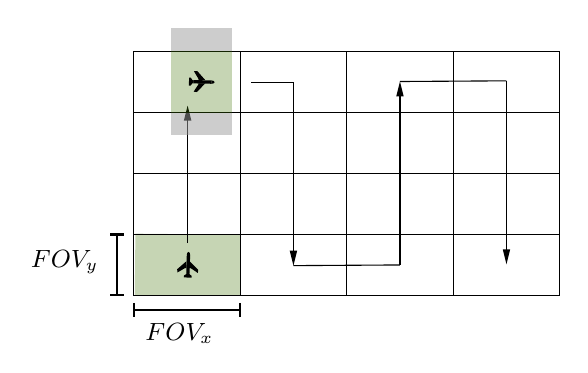
\begin{tikzpicture}[x=0.75pt,y=0.75pt,yscale=-1,xscale=1]
			%uncomment if require: \path (0,300); %set diagram left start at 0, and has height of 300
			
			%Shape: Rectangle [id:dp1592240079509375] 
			\draw  [draw opacity=0][fill={rgb, 255:red, 65; green, 117; blue, 5 }  ,fill opacity=0.3 ] (256.84,181.82) -- (307.71,182.34) -- (307.41,211.8) -- (256.54,211.29) -- cycle ;
			%Shape: Chord [id:dp027006860973721514] 
			\draw  [draw opacity=0][fill={rgb, 255:red, 0; green, 0; blue, 0 }  ,fill opacity=1 ] (281.6,192.06) .. controls (281.62,191.24) and (282,190.6) .. (282.44,190.61) .. controls (282.88,190.63) and (283.22,191.3) .. (283.2,192.11) -- cycle ;
			%Shape: Rectangle [id:dp5979870900127169] 
			\draw  [draw opacity=0][fill={rgb, 255:red, 0; green, 0; blue, 0 }  ,fill opacity=1 ] (283.2,192.11) -- (282.95,200.79) -- (281.34,200.73) -- (281.59,192.06) -- cycle ;
			%Shape: Chord [id:dp2765435991887346] 
			\draw  [draw opacity=0][fill={rgb, 255:red, 0; green, 0; blue, 0 }  ,fill opacity=1 ] (282.95,200.79) .. controls (282.92,201.6) and (282.54,202.25) .. (282.1,202.24) .. controls (281.66,202.22) and (281.32,201.55) .. (281.34,200.73) -- cycle ;
			%Shape: Boxed Polygon [id:dp6872706935659367] 
			\draw  [draw opacity=0][fill={rgb, 255:red, 0; green, 0; blue, 0 }  ,fill opacity=1 ] (286.91,200.76) -- (283.6,198.53) -- (282.91,198.32) -- (282.99,195.12) -- (287.11,199.24) -- cycle ;
			%Shape: Boxed Polygon [id:dp5311750689290109] 
			\draw  [draw opacity=0][fill={rgb, 255:red, 0; green, 0; blue, 0 }  ,fill opacity=1 ] (277.09,200.5) -- (280.62,198.47) -- (281.35,198.31) -- (281.43,195.07) -- (276.96,198.96) -- cycle ;
			%Shape: Boxed Polygon [id:dp9447821201006807] 
			\draw  [draw opacity=0][fill={rgb, 255:red, 0; green, 0; blue, 0 }  ,fill opacity=1 ] (283.98,202.18) -- (283.92,203.04) -- (280.14,202.88) -- (280.18,202.05) -- (282.14,200.76) -- cycle ;
			
			
			%Shape: Rectangle [id:dp49983792011863337] 
			\draw   (255.97,94.15) -- (307.3,94.15) -- (307.3,123.51) -- (255.97,123.51) -- cycle ;
			%Shape: Rectangle [id:dp8807821798790052] 
			\draw   (307.3,94.15) -- (358.63,94.15) -- (358.63,123.51) -- (307.3,123.51) -- cycle ;
			%Shape: Rectangle [id:dp8181512728288265] 
			\draw   (358.63,94.15) -- (409.96,94.15) -- (409.96,123.51) -- (358.63,123.51) -- cycle ;
			%Shape: Rectangle [id:dp09547819591891549] 
			\draw   (255.97,123.51) -- (307.3,123.51) -- (307.3,152.86) -- (255.97,152.86) -- cycle ;
			%Shape: Rectangle [id:dp1985429505890559] 
			\draw   (255.97,152.86) -- (307.3,152.86) -- (307.3,182.22) -- (255.97,182.22) -- cycle ;
			%Shape: Rectangle [id:dp5422527345143757] 
			\draw   (409.96,182.22) -- (461.29,182.22) -- (461.29,211.57) -- (409.96,211.57) -- cycle ;
			%Shape: Rectangle [id:dp332416764045272] 
			\draw   (307.3,123.51) -- (358.63,123.51) -- (358.63,152.86) -- (307.3,152.86) -- cycle ;
			%Shape: Rectangle [id:dp36287337689551014] 
			\draw   (307.3,152.86) -- (358.63,152.86) -- (358.63,182.22) -- (307.3,182.22) -- cycle ;
			%Shape: Rectangle [id:dp4697135024528536] 
			\draw   (358.63,152.86) -- (409.96,152.86) -- (409.96,182.22) -- (358.63,182.22) -- cycle ;
			%Shape: Rectangle [id:dp1298855569227555] 
			\draw   (358.63,123.51) -- (409.96,123.51) -- (409.96,152.86) -- (358.63,152.86) -- cycle ;
			%Shape: Rectangle [id:dp8663339040779854] 
			\draw   (255.97,182.22) -- (307.3,182.22) -- (307.3,211.57) -- (255.97,211.57) -- cycle ;
			%Shape: Rectangle [id:dp9437211813054305] 
			\draw   (307.3,182.22) -- (358.63,182.22) -- (358.63,211.57) -- (307.3,211.57) -- cycle ;
			%Shape: Rectangle [id:dp810113535837834] 
			\draw   (358.63,182.22) -- (409.96,182.22) -- (409.96,211.57) -- (358.63,211.57) -- cycle ;
			%Shape: Rectangle [id:dp5562129843015806] 
			\draw   (409.96,152.86) -- (461.29,152.86) -- (461.29,182.22) -- (409.96,182.22) -- cycle ;
			%Shape: Rectangle [id:dp8187981325254521] 
			\draw   (409.96,123.51) -- (461.29,123.51) -- (461.29,152.86) -- (409.96,152.86) -- cycle ;
			%Shape: Rectangle [id:dp6245482862531306] 
			\draw   (409.96,94.15) -- (461.29,94.15) -- (461.29,123.51) -- (409.96,123.51) -- cycle ;
			
			%Straight Lines [id:da41795839579175675] 
			\draw    (282,186.43) -- (282,122.14) ;
			\draw [shift={(282,120.14)}, rotate = 450] [fill={rgb, 255:red, 0; green, 0; blue, 0 }  ][line width=0.08]  [draw opacity=0] (7.2,-1.8) -- (0,0) -- (7.2,1.8) -- cycle    ;
			%Straight Lines [id:da1509716304633384] 
			\draw    (332.96,108.83) -- (312.68,108.83) ;
			%Straight Lines [id:da48049309446832655] 
			\draw    (332.96,108.83) -- (332.96,195.22) ;
			\draw [shift={(332.96,197.22)}, rotate = 270] [fill={rgb, 255:red, 0; green, 0; blue, 0 }  ][line width=0.08]  [draw opacity=0] (7.2,-1.8) -- (0,0) -- (7.2,1.8) -- cycle    ;
			%Straight Lines [id:da4231981271606413] 
			\draw    (384.29,196.89) -- (332.96,197.22) ;
			%Straight Lines [id:da4546308979435414] 
			\draw    (384.29,196.89) -- (384.29,110.51) ;
			\draw [shift={(384.29,108.51)}, rotate = 450] [fill={rgb, 255:red, 0; green, 0; blue, 0 }  ][line width=0.08]  [draw opacity=0] (7.2,-1.8) -- (0,0) -- (7.2,1.8) -- cycle    ;
			%Straight Lines [id:da10063088031705991] 
			\draw    (435.62,108.18) -- (384.29,108.51) ;
			%Straight Lines [id:da8147890256777217] 
			\draw    (435.62,108.18) -- (435.62,194.57) ;
			\draw [shift={(435.62,196.57)}, rotate = 270] [fill={rgb, 255:red, 0; green, 0; blue, 0 }  ][line width=0.08]  [draw opacity=0] (7.2,-1.8) -- (0,0) -- (7.2,1.8) -- cycle    ;
			%Shape: Rectangle [id:dp7310476894921445] 
			\draw  [draw opacity=0][fill={rgb, 255:red, 65; green, 117; blue, 5 }  ,fill opacity=0.3 ] (303.54,93.61) -- (303.54,123.51) -- (274.08,123.51) -- (274.08,93.61) -- cycle ;
			%Shape: Chord [id:dp19645121488474926] 
			\draw  [draw opacity=0][fill={rgb, 255:red, 0; green, 0; blue, 0 }  ,fill opacity=1 ] (293.55,107.99) .. controls (294.36,108.01) and (295.02,108.38) .. (295,108.83) .. controls (294.99,109.27) and (294.32,109.61) .. (293.51,109.6) -- cycle ;
			%Shape: Rectangle [id:dp05174583825785106] 
			\draw  [draw opacity=0][fill={rgb, 255:red, 0; green, 0; blue, 0 }  ,fill opacity=1 ] (293.51,109.6) -- (284.83,109.43) -- (284.87,107.82) -- (293.55,107.99) -- cycle ;
			%Shape: Chord [id:dp1661582095490599] 
			\draw  [draw opacity=0][fill={rgb, 255:red, 0; green, 0; blue, 0 }  ,fill opacity=1 ] (284.83,109.43) .. controls (284.02,109.42) and (283.37,109.05) .. (283.38,108.6) .. controls (283.39,108.16) and (284.06,107.81) .. (284.87,107.83) -- cycle ;
			%Shape: Boxed Polygon [id:dp018588797866418538] 
			\draw  [draw opacity=0][fill={rgb, 255:red, 0; green, 0; blue, 0 }  ,fill opacity=1 ] (284.9,113.4) -- (287.1,110.06) -- (287.3,109.37) -- (290.5,109.42) -- (286.42,113.58) -- cycle ;
			%Shape: Boxed Polygon [id:dp3166422244467362] 
			\draw  [draw opacity=0][fill={rgb, 255:red, 0; green, 0; blue, 0 }  ,fill opacity=1 ] (285.06,103.57) -- (287.13,107.09) -- (287.3,107.81) -- (290.54,107.86) -- (286.6,103.43) -- cycle ;
			%Shape: Boxed Polygon [id:dp7707267480495361] 
			\draw  [draw opacity=0][fill={rgb, 255:red, 0; green, 0; blue, 0 }  ,fill opacity=1 ] (283.45,110.48) -- (282.59,110.43) -- (282.72,106.65) -- (283.55,106.68) -- (284.85,108.63) -- cycle ;
			
			%Shape: Rectangle [id:dp26082048868605323] 
			\draw  [draw opacity=0][fill={rgb, 255:red, 155; green, 155; blue, 155 }  ,fill opacity=0.5 ] (303.58,123.51) -- (303.58,134.27) -- (274.04,134.27) -- (274.04,123.51) -- cycle ;
			%Shape: Rectangle [id:dp570071469284922] 
			\draw  [draw opacity=0][fill={rgb, 255:red, 155; green, 155; blue, 155 }  ,fill opacity=0.5 ] (303.58,82.84) -- (303.58,93.61) -- (274.04,93.61) -- (274.04,82.84) -- cycle ;
			
			%Straight Lines [id:da1628094381777676] 
			\draw    (247.97,182.22) -- (247.97,211.57) ;
			\draw [shift={(247.97,211.57)}, rotate = 270] [color={rgb, 255:red, 0; green, 0; blue, 0 }  ][line width=0.75]    (0,3.35) -- (0,-3.35)   ;
			\draw [shift={(247.97,182.22)}, rotate = 270] [color={rgb, 255:red, 0; green, 0; blue, 0 }  ][line width=0.75]    (0,3.35) -- (0,-3.35)   ;
			%Straight Lines [id:da97063001945603] 
			\draw    (255.97,218.57) -- (307.3,218.57) ;
			\draw [shift={(307.3,218.57)}, rotate = 180] [color={rgb, 255:red, 0; green, 0; blue, 0 }  ][line width=0.75]    (0,3.35) -- (0,-3.35)   ;
			\draw [shift={(255.97,218.57)}, rotate = 180] [color={rgb, 255:red, 0; green, 0; blue, 0 }  ][line width=0.75]    (0,3.35) -- (0,-3.35)   ;
			
			% Text Node
			\draw (260.4,223.8) node [anchor=north west][inner sep=0.75pt]  [font=\small]  {$FOV_{x}$};
			% Text Node
			\draw (205.2,188.6) node [anchor=north west][inner sep=0.75pt]  [font=\small]  {$FOV_{y}$};
			
			
		\end{tikzpicture}
		\caption{Rectangular discretisation}
		\label{fig:Overlap-rect}
	\end{subfigure}
	\caption{Diagrams showing cross track overlap for camera Field of View for different discretisation techniques.}
\end{figure}

% TODO: Section where it is applied to different camera scenarios

% mention how dynamic constraints change everything - with this discretisation the asumption is that UAV can make 90 degree turns. This may be possible for some UAVs, but not while maintaining a constant velocity. Maintaining constant is more desireable because it consumes les energy.



\chapter{Divide Areas Algorithm}
\label{chp:DARP}

%%%%%%%%%%%%%%%%%%%%%%%%%%%%%%%%%%%%%%%%%%%%%%%%%%%%%%%%%%%%%%%%%%%%%%%
\section{Background}
The research aim in section \ref{sec:intro_researchAim} refers to the development of a coverage path planning algorithm using multiple UAVs. Coverage path planning is often linked to applications such as surveying, mapping and searching, because it involves planning a UAVs path so as to cover all points in an environment. The idea is then that one could speed up the time taken to cover the environment mentioned by using several UAVs searching in tandem.

Before one can begin covering an area, the points within this area that must be searched require identifying. With coverage path planning, grid-based methods are quite popular because they make it easy to divide an area into searchable cells.
% TODO: Include more justification on grid based
Grid-based coverage path planning can be implemented using a number of different methods. 

Naturally, achieving the most optimal solution possible would be most desireable. The authors of \cite{DARP2017} propose a set of requirements for optimal coverage path planning using a grid-based approach. These fundamental conditions, as they call them, are listed below.

\begin{enumerate}
	\item Every cell in the environment, that is not classified as an object, must be covered. This is known as complete coverage.
	\item Each cell in the environment must only be searched once, and only by one of the robots. This is known as the non-backtracking requirement.
	\item Each robot should have as close to an equal amount of cells as possible assigned to it for searching. Their sets of cells should be of roughly the same size.
	\item The sets of cells assigned to each robot should be a connected sub-region. This means that when generating a path to search the cells within its set, a robot would not need to traverse that of another to search it's own sub-region.
	\item The initial position of each robot should be contained within the set of cells assigned to it. This means that a robot would not need to travel to reach its sub-region for searching.
\end{enumerate}
% TODO: Maybe mention something about the EXISTENCE of solutions
% Coverage
% Grid Based
% Optimize

%%%%%%%%%%%%%%%%%%%%%%%%%%%%%%%%%%%%%%%%%%%%%%%%%%%%%%%%%%%%%%%%%%%%%%%
\section{Implementation}
\subsection{Comparison of Distance Measures}

\chapter{Subregion Coverage Technique}
\label{chp:Subregion-Coverage}


%%%%%%%%%%%%%%%%%%%%%%%%%%%%%%%%%%%%%%%%%%%%%%%%%%%%%%%%%%%%%%%%%%%%%%%
\section{Background}

% Refer back to the literature review

\section{Spanning Tree Generation}

% Mention the small cells and the large cells

\section{Spanning Tree Circumnavigation}
Once the tree has been generated, the circumnavigation is achieved in two phases. Initially, a series of arrows are generated to represent a clockwise motion around the tree. This looks similar to a directed graph, because the edges are essentially assigned direction. However, because these arrows are used to generate a path for tree circumnavigation, there will be two arrows on each edge and the order in which they are used is crucial. In the second phase, these arrows are used to generate the way-points necessary to circumnavigate the tree.

A convention was formed in order to generate the arrows and way-points consistently. Firstly, once the tree is generated, a starting node is chosen. From this node, a walk is done from one node to the next to form arrows. These arrows are generated in such a way that they can be used to represent a clockwise motion around the tree. Keeping this clockwise convention in mind, way-points are generated for each arrow. 

The direction an arrow points always represents a forward motion. If the next arrow is pointing in the same direction, it is considered a forward motion. Three other motions are possible, namely left, right and backward motions. It is important to note that, although backtracking is allowed for arrows, this is not the case for the way-points. A representation of how a reference frame would move with the arrows in the event of a right turn is shown in Figure \ref{fig:ref-frame}.

\begin{figure}[h!]
	\centering
	\tikzset{every picture/.style={line width=0.75pt}} %set default line width to 0.75pt        	
	\begin{tikzpicture}[x=0.75pt,y=0.75pt,yscale=-1,xscale=1]
		%uncomment if require: \path (0,428); %set diagram left start at 0, and has height of 428
		
		%Straight Lines [id:da22962018155747188] 
		\draw [color={rgb, 255:red, 208; green, 2; blue, 27 }  ,draw opacity=1 ]   (339.88,99.5) -- (284,99.5) ;
		%Straight Lines [id:da20659579397175154] 
		\draw [color={rgb, 255:red, 208; green, 2; blue, 27 }  ,draw opacity=1 ]   (150,166) -- (150,223.94) ;
		%Straight Lines [id:da29821586315410764] 
		\draw    (90,226) -- (210,226) ;
		%Straight Lines [id:da8192544007793721] 
		\draw    (150,286) -- (150,226) ;
		%Shape: Circle [id:dp35225972894210633] 
		\draw  [draw opacity=0][fill={rgb, 255:red, 0; green, 0; blue, 0 }  ,fill opacity=1 ] (144.95,226) .. controls (144.95,223.21) and (147.21,220.95) .. (150,220.95) .. controls (152.79,220.95) and (155.05,223.21) .. (155.05,226) .. controls (155.05,228.79) and (152.79,231.05) .. (150,231.05) .. controls (147.21,231.05) and (144.95,228.79) .. (144.95,226) -- cycle ;
		%Shape: Circle [id:dp9484671919378986] 
		\draw  [fill={rgb, 255:red, 0; green, 0; blue, 0 }  ,fill opacity=1 ] (210,226) .. controls (210,224.86) and (210.92,223.94) .. (212.06,223.94) .. controls (213.2,223.94) and (214.13,224.86) .. (214.13,226) .. controls (214.13,227.14) and (213.2,228.06) .. (212.06,228.06) .. controls (210.92,228.06) and (210,227.14) .. (210,226) -- cycle ;
		%Shape: Circle [id:dp833048521369973] 
		\draw  [fill={rgb, 255:red, 0; green, 0; blue, 0 }  ,fill opacity=1 ] (147.94,286) .. controls (147.94,284.86) and (148.86,283.94) .. (150,283.94) .. controls (151.14,283.94) and (152.06,284.86) .. (152.06,286) .. controls (152.06,287.14) and (151.14,288.06) .. (150,288.06) .. controls (148.86,288.06) and (147.94,287.14) .. (147.94,286) -- cycle ;
		%Shape: Circle [id:dp5683936728423231] 
		\draw  [color={rgb, 255:red, 208; green, 2; blue, 27 }  ,draw opacity=1 ][fill={rgb, 255:red, 208; green, 2; blue, 27 }  ,fill opacity=1 ] (147.94,168.06) .. controls (147.94,166.92) and (148.86,166) .. (150,166) .. controls (151.14,166) and (152.06,166.92) .. (152.06,168.06) .. controls (152.06,169.2) and (151.14,170.13) .. (150,170.13) .. controls (148.86,170.13) and (147.94,169.2) .. (147.94,168.06) -- cycle ;
		%Shape: Circle [id:dp6006706790162355] 
		\draw  [fill={rgb, 255:red, 0; green, 0; blue, 0 }  ,fill opacity=1 ] (90,226) .. controls (90,224.86) and (90.92,223.94) .. (92.06,223.94) .. controls (93.2,223.94) and (94.13,224.86) .. (94.13,226) .. controls (94.13,227.14) and (93.2,228.06) .. (92.06,228.06) .. controls (90.92,228.06) and (90,227.14) .. (90,226) -- cycle ;
		%Straight Lines [id:da6990176420132321] 
		\draw    (284,39.5) -- (284,159.5) ;
		%Straight Lines [id:da15438188613200365] 
		\draw    (224,99.5) -- (284,99.5) ;
		%Shape: Circle [id:dp6972525301538133] 
		\draw  [draw opacity=0][fill={rgb, 255:red, 0; green, 0; blue, 0 }  ,fill opacity=1 ] (284,94.45) .. controls (286.79,94.45) and (289.05,96.71) .. (289.05,99.5) .. controls (289.05,102.29) and (286.79,104.55) .. (284,104.55) .. controls (281.21,104.55) and (278.95,102.29) .. (278.95,99.5) .. controls (278.95,96.71) and (281.21,94.45) .. (284,94.45) -- cycle ;
		%Shape: Circle [id:dp400672837370456] 
		\draw  [fill={rgb, 255:red, 0; green, 0; blue, 0 }  ,fill opacity=1 ] (284,159.5) .. controls (285.14,159.5) and (286.06,160.42) .. (286.06,161.56) .. controls (286.06,162.7) and (285.14,163.63) .. (284,163.63) .. controls (282.86,163.63) and (281.94,162.7) .. (281.94,161.56) .. controls (281.94,160.42) and (282.86,159.5) .. (284,159.5) -- cycle ;
		%Shape: Circle [id:dp8987931435704095] 
		\draw  [fill={rgb, 255:red, 0; green, 0; blue, 0 }  ,fill opacity=1 ] (224,97.44) .. controls (225.14,97.44) and (226.06,98.36) .. (226.06,99.5) .. controls (226.06,100.64) and (225.14,101.56) .. (224,101.56) .. controls (222.86,101.56) and (221.94,100.64) .. (221.94,99.5) .. controls (221.94,98.36) and (222.86,97.44) .. (224,97.44) -- cycle ;
		%Shape: Circle [id:dp9066989908899119] 
		\draw  [color={rgb, 255:red, 208; green, 2; blue, 27 }  ,draw opacity=1 ][fill={rgb, 255:red, 208; green, 2; blue, 27 }  ,fill opacity=1 ] (341.94,97.44) .. controls (343.08,97.44) and (344,98.36) .. (344,99.5) .. controls (344,100.64) and (343.08,101.56) .. (341.94,101.56) .. controls (340.8,101.56) and (339.88,100.64) .. (339.88,99.5) .. controls (339.88,98.36) and (340.8,97.44) .. (341.94,97.44) -- cycle ;
		%Shape: Circle [id:dp8606951024205995] 
		\draw  [fill={rgb, 255:red, 0; green, 0; blue, 0 }  ,fill opacity=1 ] (284,39.5) .. controls (285.14,39.5) and (286.06,40.42) .. (286.06,41.56) .. controls (286.06,42.7) and (285.14,43.63) .. (284,43.63) .. controls (282.86,43.63) and (281.94,42.7) .. (281.94,41.56) .. controls (281.94,40.42) and (282.86,39.5) .. (284,39.5) -- cycle ;
		%Straight Lines [id:da29854683273675375] 
		\draw  [dash pattern={on 4.5pt off 4.5pt}]  (150,100) -- (200,100) ;
		%Straight Lines [id:da590718802691715] 
		\draw  [dash pattern={on 4.5pt off 4.5pt}]  (150,102) -- (150,140) ;
		\draw [shift={(150,100)}, rotate = 90] [fill={rgb, 255:red, 0; green, 0; blue, 0 }  ][line width=0.08]  [draw opacity=0] (12,-3) -- (0,0) -- (12,3) -- cycle    ;
		%Straight Lines [id:da6608297236594676] 
		\draw  [dash pattern={on 4.5pt off 4.5pt}]  (360,100) -- (448,100) ;
		\draw [shift={(450,100)}, rotate = 180] [fill={rgb, 255:red, 0; green, 0; blue, 0 }  ][line width=0.08]  [draw opacity=0] (12,-3) -- (0,0) -- (12,3) -- cycle    ;
		
		% Text Node
		\draw (217,218) node [anchor=north west][inner sep=0.75pt]   [align=left] {R};
		% Text Node
		\draw (71,218) node [anchor=north west][inner sep=0.75pt]   [align=left] {L};
		% Text Node
		\draw (145,292) node [anchor=north west][inner sep=0.75pt]   [align=left] {B};
		% Text Node
		\draw (144.5,148.5) node [anchor=north west][inner sep=0.75pt]  [color={rgb, 255:red, 208; green, 2; blue, 27 }  ,opacity=1 ] [align=left] {F};
		% Text Node
		\draw (277.5,165) node [anchor=north west][inner sep=0.75pt]   [align=left] {R};
		% Text Node
		\draw (278.5,18) node [anchor=north west][inner sep=0.75pt]   [align=left] {L};
		% Text Node
		\draw (204,92.5) node [anchor=north west][inner sep=0.75pt]   [align=left] {B};
		% Text Node
		\draw (348,91.5) node [anchor=north west][inner sep=0.75pt]  [color={rgb, 255:red, 208; green, 2; blue, 27 }  ,opacity=1 ] [align=left] {F};
		
		
	\end{tikzpicture}
	\caption{Figure showing how the reference frame representing motions would move with a right turn.}
	\label{fig:ref-frame}
\end{figure}

Figure \ref{fig:grid-st} shows a grid-based representation of an environment. This square environment is divided into a four-by-four grid of large cells. Each large cell represents four smaller cells wherein the \ac{uav} will actually be moving. The dotted lines show the smaller cells. The darker black lines connect the centres of the large cells in a spanning tree. In this case, the edges all have equal weights.

To generate the arrows, the algorithm first chooses a starting node. This node is simply one of the nodes on the tree with only one edge. Of the nodes numbered in Figure \ref{fig:grid-st}, nodes 0, 10 and 13 would qualify. Assuming node 0 is chosen, the arrows can then be generated as shown in Figure \ref{fig:arrows}.

\begin{figure}[h!]
	\centering
	\tikzset{every picture/.style={line width=0.75pt}} %set default line width to 0.75pt        
	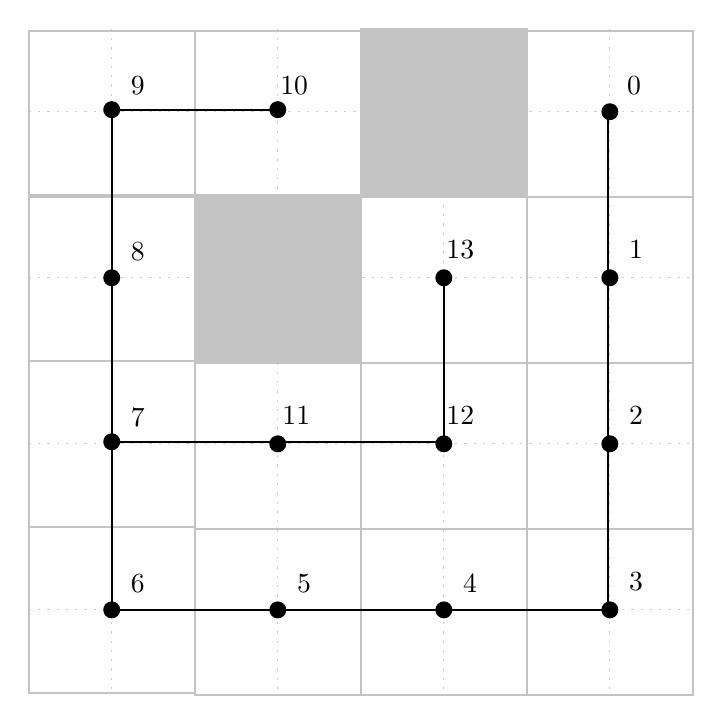
\begin{tikzpicture}[x=0.75pt,y=0.75pt,yscale=-1,xscale=1]
		%uncomment if require: \path (0,487); %set diagram left start at 0, and has height of 487
		
		%Straight Lines [id:da07078059737294629] 
		\draw [color={rgb, 255:red, 195; green, 195; blue, 195 }  ,draw opacity=0.8 ] [dash pattern={on 0.84pt off 2.51pt}]  (160,20) -- (160,340) ;
		%Straight Lines [id:da917458971819372] 
		\draw [color={rgb, 255:red, 195; green, 195; blue, 195 }  ,draw opacity=0.8 ] [dash pattern={on 0.84pt off 2.51pt}]  (240,20) -- (240,340) ;
		%Straight Lines [id:da8412450773677167] 
		\draw [color={rgb, 255:red, 195; green, 195; blue, 195 }  ,draw opacity=0.8 ] [dash pattern={on 0.84pt off 2.51pt}]  (320,20) -- (320,340) ;
		%Straight Lines [id:da3101903735332392] 
		\draw [color={rgb, 255:red, 195; green, 195; blue, 195 }  ,draw opacity=0.8 ] [dash pattern={on 0.84pt off 2.51pt}]  (400,20) -- (400,340) ;
		%Straight Lines [id:da43752561891339337] 
		\draw [color={rgb, 255:red, 195; green, 195; blue, 195 }  ,draw opacity=0.8 ] [dash pattern={on 0.84pt off 2.51pt}]  (120,60) -- (440,60) ;
		%Straight Lines [id:da21568167599612686] 
		\draw [color={rgb, 255:red, 195; green, 195; blue, 195 }  ,draw opacity=0.8 ] [dash pattern={on 0.84pt off 2.51pt}]  (120,140) -- (440,140) ;
		%Straight Lines [id:da9351274558937845] 
		\draw [color={rgb, 255:red, 195; green, 195; blue, 195 }  ,draw opacity=0.8 ] [dash pattern={on 0.84pt off 2.51pt}]  (120,220) -- (440,220) ;
		%Straight Lines [id:da8497636326794216] 
		\draw [color={rgb, 255:red, 195; green, 195; blue, 195 }  ,draw opacity=0.8 ] [dash pattern={on 0.84pt off 2.51pt}]  (120,300) -- (440,300) ;
		
		%Shape: Rectangle [id:dp7512840321055914] 
		\draw  [color={rgb, 255:red, 195; green, 195; blue, 195 }  ,draw opacity=1 ][line width=0.75]  (360,21) -- (440,21) -- (440,101) -- (360,101) -- cycle ;
		%Shape: Rectangle [id:dp08998875837998588] 
		\draw  [color={rgb, 255:red, 195; green, 195; blue, 195 }  ,draw opacity=1 ][line width=0.75]  (360,101) -- (440,101) -- (440,181) -- (360,181) -- cycle ;
		%Shape: Rectangle [id:dp0951355467677828] 
		\draw  [color={rgb, 255:red, 195; green, 195; blue, 195 }  ,draw opacity=1 ][line width=0.75]  (360,181) -- (440,181) -- (440,261) -- (360,261) -- cycle ;
		%Shape: Rectangle [id:dp7521114125139936] 
		\draw  [color={rgb, 255:red, 195; green, 195; blue, 195 }  ,draw opacity=1 ][line width=0.75]  (360,261) -- (440,261) -- (440,341) -- (360,341) -- cycle ;
		%Shape: Rectangle [id:dp7559961198567777] 
		\draw  [color={rgb, 255:red, 195; green, 195; blue, 195 }  ,draw opacity=1 ][line width=0.75]  (280,101) -- (360,101) -- (360,181) -- (280,181) -- cycle ;
		%Shape: Rectangle [id:dp8869961360769938] 
		\draw  [color={rgb, 255:red, 195; green, 195; blue, 195 }  ,draw opacity=1 ][line width=0.75]  (280,181) -- (360,181) -- (360,261) -- (280,261) -- cycle ;
		%Shape: Rectangle [id:dp5037977259529054] 
		\draw  [color={rgb, 255:red, 195; green, 195; blue, 195 }  ,draw opacity=1 ][line width=0.75]  (280,261) -- (360,261) -- (360,341) -- (280,341) -- cycle ;
		%Shape: Rectangle [id:dp773885446585411] 
		\draw  [color={rgb, 255:red, 195; green, 195; blue, 195 }  ,draw opacity=1 ][line width=0.75]  (200,21) -- (280,21) -- (280,101) -- (200,101) -- cycle ;
		%Shape: Rectangle [id:dp2052220638960709] 
		\draw  [color={rgb, 255:red, 195; green, 195; blue, 195 }  ,draw opacity=1 ][line width=0.75]  (120,21) -- (200,21) -- (200,101) -- (120,101) -- cycle ;
		%Shape: Rectangle [id:dp7105833624892055] 
		\draw  [color={rgb, 255:red, 195; green, 195; blue, 195 }  ,draw opacity=1 ][line width=0.75]  (120,100) -- (200,100) -- (200,180) -- (120,180) -- cycle ;
		%Shape: Rectangle [id:dp25180360725760975] 
		\draw  [color={rgb, 255:red, 195; green, 195; blue, 195 }  ,draw opacity=1 ][line width=0.75]  (120,180) -- (200,180) -- (200,260) -- (120,260) -- cycle ;
		%Shape: Rectangle [id:dp8614444924044413] 
		\draw  [color={rgb, 255:red, 195; green, 195; blue, 195 }  ,draw opacity=1 ][line width=0.75]  (120,260) -- (200,260) -- (200,340) -- (120,340) -- cycle ;
		%Shape: Rectangle [id:dp8378559698110666] 
		\draw  [color={rgb, 255:red, 195; green, 195; blue, 195 }  ,draw opacity=1 ][line width=0.75]  (200,181) -- (280,181) -- (280,261) -- (200,261) -- cycle ;
		%Shape: Rectangle [id:dp8380708528890195] 
		\draw  [color={rgb, 255:red, 195; green, 195; blue, 195 }  ,draw opacity=1 ][line width=0.75]  (200,261) -- (280,261) -- (280,341) -- (200,341) -- cycle ;
		
		%Straight Lines [id:da1979706309085778] 
		\draw [color={rgb, 255:red, 0; green, 0; blue, 0 }  ,draw opacity=1 ][line width=0.75]    (160,299) -- (160,59) ;
		%Shape: Rectangle [id:dp7251933800186736] 
		\draw  [color={rgb, 255:red, 195; green, 195; blue, 195 }  ,draw opacity=1 ][fill={rgb, 255:red, 195; green, 195; blue, 195 }  ,fill opacity=1 ][line width=0.75]  (280,20) -- (360,20) -- (360,100) -- (280,100) -- cycle ;
		%Shape: Rectangle [id:dp1925911620328833] 
		\draw  [color={rgb, 255:red, 195; green, 195; blue, 195 }  ,draw opacity=1 ][fill={rgb, 255:red, 195; green, 195; blue, 195 }  ,fill opacity=1 ][line width=0.75]  (200,100) -- (280,100) -- (280,180) -- (200,180) -- cycle ;
		%Straight Lines [id:da0581482096059478] 
		\draw [color={rgb, 255:red, 0; green, 0; blue, 0 }  ,draw opacity=1 ][line width=0.75]    (160,300) -- (400,300) ;
		%Straight Lines [id:da8084405416238001] 
		\draw [color={rgb, 255:red, 0; green, 0; blue, 0 }  ,draw opacity=1 ][line width=0.75]    (160,59) -- (240,59) ;
		%Straight Lines [id:da41325892147339616] 
		\draw [color={rgb, 255:red, 0; green, 0; blue, 0 }  ,draw opacity=1 ][fill={rgb, 255:red, 155; green, 155; blue, 155 }  ,fill opacity=1 ][line width=0.75]    (160,219) -- (320,219) ;
		%Straight Lines [id:da0985686119799063] 
		\draw [color={rgb, 255:red, 0; green, 0; blue, 0 }  ,draw opacity=1 ][line width=0.75]    (320,220) -- (320,140) ;
		%Straight Lines [id:da3298203658421879] 
		\draw [color={rgb, 255:red, 0; green, 0; blue, 0 }  ,draw opacity=1 ][line width=0.75]    (399,300) -- (399,60) ;
		%Shape: Circle [id:dp41582492626714096] 
		\draw  [color={rgb, 255:red, 0; green, 0; blue, 0 }  ,draw opacity=1 ][fill={rgb, 255:red, 0; green, 0; blue, 0 }  ,fill opacity=1 ] (236.19,59) .. controls (236.19,56.89) and (237.89,55.19) .. (240,55.19) .. controls (242.11,55.19) and (243.81,56.89) .. (243.81,59) .. controls (243.81,61.11) and (242.11,62.81) .. (240,62.81) .. controls (237.89,62.81) and (236.19,61.11) .. (236.19,59) -- cycle ;
		%Shape: Circle [id:dp5558894380647834] 
		\draw  [color={rgb, 255:red, 0; green, 0; blue, 0 }  ,draw opacity=1 ][fill={rgb, 255:red, 0; green, 0; blue, 0 }  ,fill opacity=1 ] (156.19,59) .. controls (156.19,56.89) and (157.89,55.19) .. (160,55.19) .. controls (162.11,55.19) and (163.81,56.89) .. (163.81,59) .. controls (163.81,61.11) and (162.11,62.81) .. (160,62.81) .. controls (157.89,62.81) and (156.19,61.11) .. (156.19,59) -- cycle ;
		%Shape: Circle [id:dp8351577385814617] 
		\draw  [color={rgb, 255:red, 0; green, 0; blue, 0 }  ,draw opacity=1 ][fill={rgb, 255:red, 0; green, 0; blue, 0 }  ,fill opacity=1 ] (396.19,60) .. controls (396.19,57.89) and (397.89,56.19) .. (400,56.19) .. controls (402.11,56.19) and (403.81,57.89) .. (403.81,60) .. controls (403.81,62.11) and (402.11,63.81) .. (400,63.81) .. controls (397.89,63.81) and (396.19,62.11) .. (396.19,60) -- cycle ;
		%Shape: Circle [id:dp7940426606232267] 
		\draw  [color={rgb, 255:red, 0; green, 0; blue, 0 }  ,draw opacity=1 ][fill={rgb, 255:red, 0; green, 0; blue, 0 }  ,fill opacity=1 ] (316.19,140) .. controls (316.19,137.89) and (317.89,136.19) .. (320,136.19) .. controls (322.11,136.19) and (323.81,137.89) .. (323.81,140) .. controls (323.81,142.11) and (322.11,143.81) .. (320,143.81) .. controls (317.89,143.81) and (316.19,142.11) .. (316.19,140) -- cycle ;
		%Shape: Circle [id:dp04520481160188616] 
		\draw  [color={rgb, 255:red, 0; green, 0; blue, 0 }  ,draw opacity=1 ][fill={rgb, 255:red, 0; green, 0; blue, 0 }  ,fill opacity=1 ] (316.19,220) .. controls (316.19,217.89) and (317.89,216.19) .. (320,216.19) .. controls (322.11,216.19) and (323.81,217.89) .. (323.81,220) .. controls (323.81,222.11) and (322.11,223.81) .. (320,223.81) .. controls (317.89,223.81) and (316.19,222.11) .. (316.19,220) -- cycle ;
		%Shape: Circle [id:dp5073699623939971] 
		\draw  [color={rgb, 255:red, 0; green, 0; blue, 0 }  ,draw opacity=1 ][fill={rgb, 255:red, 0; green, 0; blue, 0 }  ,fill opacity=1 ] (236.19,220) .. controls (236.19,217.89) and (237.89,216.19) .. (240,216.19) .. controls (242.11,216.19) and (243.81,217.89) .. (243.81,220) .. controls (243.81,222.11) and (242.11,223.81) .. (240,223.81) .. controls (237.89,223.81) and (236.19,222.11) .. (236.19,220) -- cycle ;
		%Shape: Circle [id:dp2213240590117067] 
		\draw  [color={rgb, 255:red, 0; green, 0; blue, 0 }  ,draw opacity=1 ][fill={rgb, 255:red, 0; green, 0; blue, 0 }  ,fill opacity=1 ] (156.19,219) .. controls (156.19,216.89) and (157.89,215.19) .. (160,215.19) .. controls (162.11,215.19) and (163.81,216.89) .. (163.81,219) .. controls (163.81,221.11) and (162.11,222.81) .. (160,222.81) .. controls (157.89,222.81) and (156.19,221.11) .. (156.19,219) -- cycle ;
		%Shape: Circle [id:dp979294341687238] 
		\draw  [color={rgb, 255:red, 0; green, 0; blue, 0 }  ,draw opacity=1 ][fill={rgb, 255:red, 0; green, 0; blue, 0 }  ,fill opacity=1 ] (156.19,140) .. controls (156.19,137.89) and (157.89,136.19) .. (160,136.19) .. controls (162.11,136.19) and (163.81,137.89) .. (163.81,140) .. controls (163.81,142.11) and (162.11,143.81) .. (160,143.81) .. controls (157.89,143.81) and (156.19,142.11) .. (156.19,140) -- cycle ;
		%Shape: Circle [id:dp14676659616041077] 
		\draw  [color={rgb, 255:red, 0; green, 0; blue, 0 }  ,draw opacity=1 ][fill={rgb, 255:red, 0; green, 0; blue, 0 }  ,fill opacity=1 ] (396.19,140) .. controls (396.19,137.89) and (397.89,136.19) .. (400,136.19) .. controls (402.11,136.19) and (403.81,137.89) .. (403.81,140) .. controls (403.81,142.11) and (402.11,143.81) .. (400,143.81) .. controls (397.89,143.81) and (396.19,142.11) .. (396.19,140) -- cycle ;
		%Shape: Circle [id:dp19334338983125243] 
		\draw  [color={rgb, 255:red, 0; green, 0; blue, 0 }  ,draw opacity=1 ][fill={rgb, 255:red, 0; green, 0; blue, 0 }  ,fill opacity=1 ] (396.19,220) .. controls (396.19,217.89) and (397.89,216.19) .. (400,216.19) .. controls (402.11,216.19) and (403.81,217.89) .. (403.81,220) .. controls (403.81,222.11) and (402.11,223.81) .. (400,223.81) .. controls (397.89,223.81) and (396.19,222.11) .. (396.19,220) -- cycle ;
		%Shape: Circle [id:dp5263269612866854] 
		\draw  [color={rgb, 255:red, 0; green, 0; blue, 0 }  ,draw opacity=1 ][fill={rgb, 255:red, 0; green, 0; blue, 0 }  ,fill opacity=1 ] (396.19,300) .. controls (396.19,297.89) and (397.89,296.19) .. (400,296.19) .. controls (402.11,296.19) and (403.81,297.89) .. (403.81,300) .. controls (403.81,302.11) and (402.11,303.81) .. (400,303.81) .. controls (397.89,303.81) and (396.19,302.11) .. (396.19,300) -- cycle ;
		%Shape: Circle [id:dp41455563786620653] 
		\draw  [color={rgb, 255:red, 0; green, 0; blue, 0 }  ,draw opacity=1 ][fill={rgb, 255:red, 0; green, 0; blue, 0 }  ,fill opacity=1 ] (316.19,300) .. controls (316.19,297.89) and (317.89,296.19) .. (320,296.19) .. controls (322.11,296.19) and (323.81,297.89) .. (323.81,300) .. controls (323.81,302.11) and (322.11,303.81) .. (320,303.81) .. controls (317.89,303.81) and (316.19,302.11) .. (316.19,300) -- cycle ;
		%Shape: Circle [id:dp9746259257783465] 
		\draw  [color={rgb, 255:red, 0; green, 0; blue, 0 }  ,draw opacity=1 ][fill={rgb, 255:red, 0; green, 0; blue, 0 }  ,fill opacity=1 ] (236.19,300) .. controls (236.19,297.89) and (237.89,296.19) .. (240,296.19) .. controls (242.11,296.19) and (243.81,297.89) .. (243.81,300) .. controls (243.81,302.11) and (242.11,303.81) .. (240,303.81) .. controls (237.89,303.81) and (236.19,302.11) .. (236.19,300) -- cycle ;
		%Shape: Circle [id:dp5753636930291428] 
		\draw  [color={rgb, 255:red, 0; green, 0; blue, 0 }  ,draw opacity=1 ][fill={rgb, 255:red, 0; green, 0; blue, 0 }  ,fill opacity=1 ] (156.19,300) .. controls (156.19,297.89) and (157.89,296.19) .. (160,296.19) .. controls (162.11,296.19) and (163.81,297.89) .. (163.81,300) .. controls (163.81,302.11) and (162.11,303.81) .. (160,303.81) .. controls (157.89,303.81) and (156.19,302.11) .. (156.19,300) -- cycle ;
		
		% Text Node
		\draw (407,42) node [anchor=north west][inner sep=0.75pt]   [align=left] {0};
		% Text Node
		\draw (408,121) node [anchor=north west][inner sep=0.75pt]   [align=left] {1};
		% Text Node
		\draw (408,201) node [anchor=north west][inner sep=0.75pt]   [align=left] {2};
		% Text Node
		\draw (408,281) node [anchor=north west][inner sep=0.75pt]   [align=left] {3};
		% Text Node
		\draw (328,282) node [anchor=north west][inner sep=0.75pt]   [align=left] {4};
		% Text Node
		\draw (248,282) node [anchor=north west][inner sep=0.75pt]   [align=left] {5};
		% Text Node
		\draw (168,282) node [anchor=north west][inner sep=0.75pt]   [align=left] {6};
		% Text Node
		\draw (168,202) node [anchor=north west][inner sep=0.75pt]   [align=left] {7};
		% Text Node
		\draw (168,122) node [anchor=north west][inner sep=0.75pt]   [align=left] {8};
		% Text Node
		\draw (168,42) node [anchor=north west][inner sep=0.75pt]   [align=left] {9};
		% Text Node
		\draw (240,42) node [anchor=north west][inner sep=0.75pt]   [align=left] {10};
		% Text Node
		\draw (241,201) node [anchor=north west][inner sep=0.75pt]   [align=left] {11};
		% Text Node
		\draw (320,201) node [anchor=north west][inner sep=0.75pt]   [align=left] {12};
		% Text Node
		\draw (320,121) node [anchor=north west][inner sep=0.75pt]   [align=left] {13};
		
		
	\end{tikzpicture}
	\caption{Figure showing a spanning tree generated for a four-by-four environment grid}
	\label{fig:grid-st}
\end{figure}

\begin{figure}[h!]
	\centering
	\tikzset{every picture/.style={line width=0.75pt}} %set default line width to 0.75pt        
	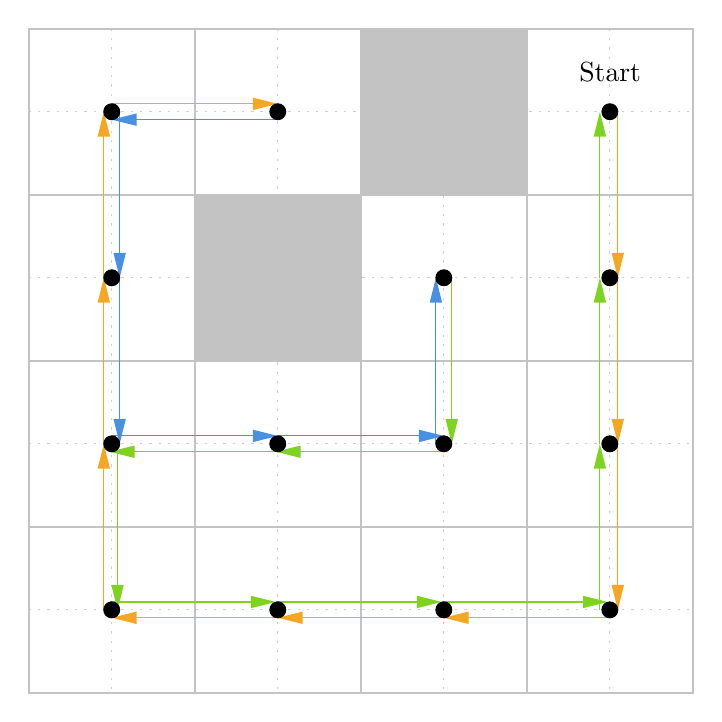
\begin{tikzpicture}[x=0.75pt,y=0.75pt,yscale=-1,xscale=1]
		%uncomment if require: \path (0,487); %set diagram left start at 0, and has height of 487
		
		%Straight Lines [id:da3977750045093258] 
		\draw [color={rgb, 255:red, 195; green, 195; blue, 195 }  ,draw opacity=0.8 ] [dash pattern={on 0.84pt off 2.51pt}]  (160,20) -- (160,340) ;
		%Straight Lines [id:da07618883915401731] 
		\draw [color={rgb, 255:red, 195; green, 195; blue, 195 }  ,draw opacity=0.8 ] [dash pattern={on 0.84pt off 2.51pt}]  (240,20) -- (240,340) ;
		%Straight Lines [id:da06600432409341517] 
		\draw [color={rgb, 255:red, 195; green, 195; blue, 195 }  ,draw opacity=0.8 ] [dash pattern={on 0.84pt off 2.51pt}]  (320,20) -- (320,340) ;
		%Straight Lines [id:da5290784258779333] 
		\draw [color={rgb, 255:red, 195; green, 195; blue, 195 }  ,draw opacity=0.8 ] [dash pattern={on 0.84pt off 2.51pt}]  (400,20) -- (400,340) ;
		%Straight Lines [id:da9833595064287617] 
		\draw [color={rgb, 255:red, 195; green, 195; blue, 195 }  ,draw opacity=0.8 ] [dash pattern={on 0.84pt off 2.51pt}]  (120,60) -- (440,60) ;
		%Straight Lines [id:da520432231001738] 
		\draw [color={rgb, 255:red, 195; green, 195; blue, 195 }  ,draw opacity=0.8 ] [dash pattern={on 0.84pt off 2.51pt}]  (120,140) -- (440,140) ;
		%Straight Lines [id:da6002867106183594] 
		\draw [color={rgb, 255:red, 195; green, 195; blue, 195 }  ,draw opacity=0.8 ] [dash pattern={on 0.84pt off 2.51pt}]  (120,220) -- (440,220) ;
		%Straight Lines [id:da9782745721301296] 
		\draw [color={rgb, 255:red, 195; green, 195; blue, 195 }  ,draw opacity=0.8 ] [dash pattern={on 0.84pt off 2.51pt}]  (120,300) -- (440,300) ;
		
		%Shape: Rectangle [id:dp5898184612923194] 
		\draw  [color={rgb, 255:red, 195; green, 195; blue, 195 }  ,draw opacity=1 ][line width=0.75]  (360,20) -- (440,20) -- (440,100) -- (360,100) -- cycle ;
		%Shape: Rectangle [id:dp48862096625716034] 
		\draw  [color={rgb, 255:red, 195; green, 195; blue, 195 }  ,draw opacity=1 ][line width=0.75]  (360,100) -- (440,100) -- (440,180) -- (360,180) -- cycle ;
		%Shape: Rectangle [id:dp3755148108063808] 
		\draw  [color={rgb, 255:red, 195; green, 195; blue, 195 }  ,draw opacity=1 ][line width=0.75]  (360,180) -- (440,180) -- (440,260) -- (360,260) -- cycle ;
		%Shape: Rectangle [id:dp9473736210218475] 
		\draw  [color={rgb, 255:red, 195; green, 195; blue, 195 }  ,draw opacity=1 ][line width=0.75]  (360,260) -- (440,260) -- (440,340) -- (360,340) -- cycle ;
		%Shape: Rectangle [id:dp12436408430349899] 
		\draw  [color={rgb, 255:red, 195; green, 195; blue, 195 }  ,draw opacity=1 ][line width=0.75]  (280,100) -- (360,100) -- (360,180) -- (280,180) -- cycle ;
		%Shape: Rectangle [id:dp43828113255227175] 
		\draw  [color={rgb, 255:red, 195; green, 195; blue, 195 }  ,draw opacity=1 ][line width=0.75]  (280,180) -- (360,180) -- (360,260) -- (280,260) -- cycle ;
		%Shape: Rectangle [id:dp7405502584040733] 
		\draw  [color={rgb, 255:red, 195; green, 195; blue, 195 }  ,draw opacity=1 ][line width=0.75]  (280,260) -- (360,260) -- (360,340) -- (280,340) -- cycle ;
		%Shape: Rectangle [id:dp05296394236381641] 
		\draw  [color={rgb, 255:red, 195; green, 195; blue, 195 }  ,draw opacity=1 ][line width=0.75]  (120,20) -- (200,20) -- (200,100) -- (120,100) -- cycle ;
		%Shape: Rectangle [id:dp6150857421701121] 
		\draw  [color={rgb, 255:red, 195; green, 195; blue, 195 }  ,draw opacity=1 ][line width=0.75]  (120,100) -- (200,100) -- (200,180) -- (120,180) -- cycle ;
		%Shape: Rectangle [id:dp5861189397744904] 
		\draw  [color={rgb, 255:red, 195; green, 195; blue, 195 }  ,draw opacity=1 ][line width=0.75]  (120,180) -- (200,180) -- (200,260) -- (120,260) -- cycle ;
		%Shape: Rectangle [id:dp8672396938760043] 
		\draw  [color={rgb, 255:red, 195; green, 195; blue, 195 }  ,draw opacity=1 ][line width=0.75]  (120,260) -- (200,260) -- (200,340) -- (120,340) -- cycle ;
		%Shape: Rectangle [id:dp32997979058045] 
		\draw  [color={rgb, 255:red, 195; green, 195; blue, 195 }  ,draw opacity=1 ][line width=0.75]  (200,180) -- (280,180) -- (280,260) -- (200,260) -- cycle ;
		%Shape: Rectangle [id:dp6083880745681156] 
		\draw  [color={rgb, 255:red, 195; green, 195; blue, 195 }  ,draw opacity=1 ][line width=0.75]  (200,260) -- (280,260) -- (280,340) -- (200,340) -- cycle ;
		
		%Shape: Rectangle [id:dp6989257767580808] 
		\draw  [color={rgb, 255:red, 195; green, 195; blue, 195 }  ,draw opacity=1 ][line width=0.75]  (200,20) -- (280,20) -- (280,100) -- (200,100) -- cycle ;
		
		%Shape: Rectangle [id:dp3496282639540844] 
		\draw  [color={rgb, 255:red, 195; green, 195; blue, 195 }  ,draw opacity=1 ][fill={rgb, 255:red, 195; green, 195; blue, 195 }  ,fill opacity=1 ][line width=0.75]  (280,20) -- (360,20) -- (360,100) -- (280,100) -- cycle ;
		%Shape: Rectangle [id:dp1101274608527989] 
		\draw  [color={rgb, 255:red, 195; green, 195; blue, 195 }  ,draw opacity=1 ][fill={rgb, 255:red, 195; green, 195; blue, 195 }  ,fill opacity=1 ][line width=0.75]  (200,100) -- (280,100) -- (280,180) -- (200,180) -- cycle ;
		%Straight Lines [id:da7109877053031188] 
		\draw [color={rgb, 255:red, 245; green, 166; blue, 35 }  ,draw opacity=1 ]   (403.81,60) -- (403.81,138) ;
		\draw [shift={(403.81,140)}, rotate = 270] [fill={rgb, 255:red, 245; green, 166; blue, 35 }  ,fill opacity=1 ][line width=0.08]  [draw opacity=0] (12,-3) -- (0,0) -- (12,3) -- cycle    ;
		%Straight Lines [id:da26602598944672584] 
		\draw [color={rgb, 255:red, 126; green, 211; blue, 33 }  ,draw opacity=1 ]   (395.19,140) -- (395.19,62) ;
		\draw [shift={(395.19,60)}, rotate = 450] [fill={rgb, 255:red, 126; green, 211; blue, 33 }  ,fill opacity=1 ][line width=0.08]  [draw opacity=0] (12,-3) -- (0,0) -- (12,3) -- cycle    ;
		%Straight Lines [id:da02914591351940765] 
		\draw [color={rgb, 255:red, 126; green, 211; blue, 33 }  ,draw opacity=1 ]   (395.19,220) -- (395.19,142) ;
		\draw [shift={(395.19,140)}, rotate = 450] [fill={rgb, 255:red, 126; green, 211; blue, 33 }  ,fill opacity=1 ][line width=0.08]  [draw opacity=0] (12,-3) -- (0,0) -- (12,3) -- cycle    ;
		%Straight Lines [id:da39308513285178037] 
		\draw [color={rgb, 255:red, 245; green, 166; blue, 35 }  ,draw opacity=1 ]   (403.81,140) -- (403.81,218) ;
		\draw [shift={(403.81,220)}, rotate = 270] [fill={rgb, 255:red, 245; green, 166; blue, 35 }  ,fill opacity=1 ][line width=0.08]  [draw opacity=0] (12,-3) -- (0,0) -- (12,3) -- cycle    ;
		%Straight Lines [id:da5373248798431745] 
		\draw [color={rgb, 255:red, 245; green, 166; blue, 35 }  ,draw opacity=1 ]   (403.81,220) -- (403.81,298) ;
		\draw [shift={(403.81,300)}, rotate = 270] [fill={rgb, 255:red, 245; green, 166; blue, 35 }  ,fill opacity=1 ][line width=0.08]  [draw opacity=0] (12,-3) -- (0,0) -- (12,3) -- cycle    ;
		%Straight Lines [id:da6507397451478356] 
		\draw [color={rgb, 255:red, 126; green, 211; blue, 33 }  ,draw opacity=1 ]   (395.19,300) -- (395.19,222) ;
		\draw [shift={(395.19,220)}, rotate = 450] [fill={rgb, 255:red, 126; green, 211; blue, 33 }  ,fill opacity=1 ][line width=0.08]  [draw opacity=0] (12,-3) -- (0,0) -- (12,3) -- cycle    ;
		%Straight Lines [id:da4490944583331955] 
		\draw [color={rgb, 255:red, 245; green, 166; blue, 35 }  ,draw opacity=1 ]   (400,303.81) -- (322,303.81) ;
		\draw [shift={(320,303.81)}, rotate = 360] [fill={rgb, 255:red, 245; green, 166; blue, 35 }  ,fill opacity=1 ][line width=0.08]  [draw opacity=0] (12,-3) -- (0,0) -- (12,3) -- cycle    ;
		%Straight Lines [id:da771333880279802] 
		\draw [color={rgb, 255:red, 245; green, 166; blue, 35 }  ,draw opacity=1 ]   (320,303.81) -- (242,303.81) ;
		\draw [shift={(240,303.81)}, rotate = 360] [fill={rgb, 255:red, 245; green, 166; blue, 35 }  ,fill opacity=1 ][line width=0.08]  [draw opacity=0] (12,-3) -- (0,0) -- (12,3) -- cycle    ;
		%Straight Lines [id:da0915527602751669] 
		\draw [color={rgb, 255:red, 245; green, 166; blue, 35 }  ,draw opacity=1 ]   (240,303.81) -- (162,303.81) ;
		\draw [shift={(160,303.81)}, rotate = 360] [fill={rgb, 255:red, 245; green, 166; blue, 35 }  ,fill opacity=1 ][line width=0.08]  [draw opacity=0] (12,-3) -- (0,0) -- (12,3) -- cycle    ;
		%Straight Lines [id:da8183550519262464] 
		\draw [color={rgb, 255:red, 126; green, 211; blue, 33 }  ,draw opacity=1 ]   (319,296.19) -- (397,296.19) ;
		\draw [shift={(399,296.19)}, rotate = 180] [fill={rgb, 255:red, 126; green, 211; blue, 33 }  ,fill opacity=1 ][line width=0.08]  [draw opacity=0] (12,-3) -- (0,0) -- (12,3) -- cycle    ;
		%Straight Lines [id:da270699769832347] 
		\draw [color={rgb, 255:red, 126; green, 211; blue, 33 }  ,draw opacity=1 ]   (239,296.19) -- (317,296.19) ;
		\draw [shift={(319,296.19)}, rotate = 180] [fill={rgb, 255:red, 126; green, 211; blue, 33 }  ,fill opacity=1 ][line width=0.08]  [draw opacity=0] (12,-3) -- (0,0) -- (12,3) -- cycle    ;
		%Straight Lines [id:da5296508036432168] 
		\draw [color={rgb, 255:red, 126; green, 211; blue, 33 }  ,draw opacity=1 ]   (159,296.19) -- (237,296.19) ;
		\draw [shift={(239,296.19)}, rotate = 180] [fill={rgb, 255:red, 126; green, 211; blue, 33 }  ,fill opacity=1 ][line width=0.08]  [draw opacity=0] (12,-3) -- (0,0) -- (12,3) -- cycle    ;
		%Straight Lines [id:da6152908850819139] 
		\draw [color={rgb, 255:red, 245; green, 166; blue, 35 }  ,draw opacity=1 ]   (156.19,300) -- (156.19,222) ;
		\draw [shift={(156.19,220)}, rotate = 450] [fill={rgb, 255:red, 245; green, 166; blue, 35 }  ,fill opacity=1 ][line width=0.08]  [draw opacity=0] (12,-3) -- (0,0) -- (12,3) -- cycle    ;
		%Straight Lines [id:da4869759720464193] 
		\draw [color={rgb, 255:red, 245; green, 166; blue, 35 }  ,draw opacity=1 ]   (160,56.19) -- (238,56.19) ;
		\draw [shift={(240,56.19)}, rotate = 180] [fill={rgb, 255:red, 245; green, 166; blue, 35 }  ,fill opacity=1 ][line width=0.08]  [draw opacity=0] (12,-3) -- (0,0) -- (12,3) -- cycle    ;
		%Straight Lines [id:da41392688240238984] 
		\draw [color={rgb, 255:red, 74; green, 144; blue, 226 }  ,draw opacity=1 ]   (240,63.81) -- (162,63.81) ;
		\draw [shift={(160,63.81)}, rotate = 360] [fill={rgb, 255:red, 74; green, 144; blue, 226 }  ,fill opacity=1 ][line width=0.08]  [draw opacity=0] (12,-3) -- (0,0) -- (12,3) -- cycle    ;
		%Straight Lines [id:da1371170506661339] 
		\draw [color={rgb, 255:red, 126; green, 211; blue, 33 }  ,draw opacity=1 ]   (162.81,220) -- (162.81,298) ;
		\draw [shift={(162.81,300)}, rotate = 270] [fill={rgb, 255:red, 126; green, 211; blue, 33 }  ,fill opacity=1 ][line width=0.08]  [draw opacity=0] (12,-3) -- (0,0) -- (12,3) -- cycle    ;
		%Straight Lines [id:da06913212613382202] 
		\draw [color={rgb, 255:red, 74; green, 144; blue, 226 }  ,draw opacity=1 ]   (160,216.19) -- (238,216.19) ;
		\draw [shift={(240,216.19)}, rotate = 180] [fill={rgb, 255:red, 74; green, 144; blue, 226 }  ,fill opacity=1 ][line width=0.08]  [draw opacity=0] (12,-3) -- (0,0) -- (12,3) -- cycle    ;
		%Straight Lines [id:da37746092338955006] 
		\draw [color={rgb, 255:red, 126; green, 211; blue, 33 }  ,draw opacity=1 ]   (239,223.81) -- (161,223.81) ;
		\draw [shift={(159,223.81)}, rotate = 360] [fill={rgb, 255:red, 126; green, 211; blue, 33 }  ,fill opacity=1 ][line width=0.08]  [draw opacity=0] (12,-3) -- (0,0) -- (12,3) -- cycle    ;
		%Straight Lines [id:da5502420093118436] 
		\draw [color={rgb, 255:red, 126; green, 211; blue, 33 }  ,draw opacity=1 ]   (319,223.81) -- (241,223.81) ;
		\draw [shift={(239,223.81)}, rotate = 360] [fill={rgb, 255:red, 126; green, 211; blue, 33 }  ,fill opacity=1 ][line width=0.08]  [draw opacity=0] (12,-3) -- (0,0) -- (12,3) -- cycle    ;
		%Straight Lines [id:da25223475086499536] 
		\draw [color={rgb, 255:red, 74; green, 144; blue, 226 }  ,draw opacity=1 ]   (240,216.19) -- (318,216.19) ;
		\draw [shift={(320,216.19)}, rotate = 180] [fill={rgb, 255:red, 74; green, 144; blue, 226 }  ,fill opacity=1 ][line width=0.08]  [draw opacity=0] (12,-3) -- (0,0) -- (12,3) -- cycle    ;
		%Straight Lines [id:da8200476146784395] 
		\draw [color={rgb, 255:red, 74; green, 144; blue, 226 }  ,draw opacity=1 ]   (316.19,220) -- (316.19,142) ;
		\draw [shift={(316.19,140)}, rotate = 450] [fill={rgb, 255:red, 74; green, 144; blue, 226 }  ,fill opacity=1 ][line width=0.08]  [draw opacity=0] (12,-3) -- (0,0) -- (12,3) -- cycle    ;
		%Straight Lines [id:da5178980162476476] 
		\draw [color={rgb, 255:red, 126; green, 211; blue, 33 }  ,draw opacity=1 ]   (323.81,140) -- (323.81,218) ;
		\draw [shift={(323.81,220)}, rotate = 270] [fill={rgb, 255:red, 126; green, 211; blue, 33 }  ,fill opacity=1 ][line width=0.08]  [draw opacity=0] (12,-3) -- (0,0) -- (12,3) -- cycle    ;
		%Straight Lines [id:da5994423368626156] 
		\draw [color={rgb, 255:red, 245; green, 166; blue, 35 }  ,draw opacity=1 ]   (156.19,220) -- (156.19,142) ;
		\draw [shift={(156.19,140)}, rotate = 450] [fill={rgb, 255:red, 245; green, 166; blue, 35 }  ,fill opacity=1 ][line width=0.08]  [draw opacity=0] (12,-3) -- (0,0) -- (12,3) -- cycle    ;
		%Straight Lines [id:da2748369034984963] 
		\draw [color={rgb, 255:red, 74; green, 144; blue, 226 }  ,draw opacity=1 ]   (163.81,140) -- (163.81,218) ;
		\draw [shift={(163.81,220)}, rotate = 270] [fill={rgb, 255:red, 74; green, 144; blue, 226 }  ,fill opacity=1 ][line width=0.08]  [draw opacity=0] (12,-3) -- (0,0) -- (12,3) -- cycle    ;
		%Straight Lines [id:da6753173854185068] 
		\draw [color={rgb, 255:red, 74; green, 144; blue, 226 }  ,draw opacity=1 ]   (163.81,60) -- (163.81,138) ;
		\draw [shift={(163.81,140)}, rotate = 270] [fill={rgb, 255:red, 74; green, 144; blue, 226 }  ,fill opacity=1 ][line width=0.08]  [draw opacity=0] (12,-3) -- (0,0) -- (12,3) -- cycle    ;
		%Straight Lines [id:da6119419475380783] 
		\draw [color={rgb, 255:red, 245; green, 166; blue, 35 }  ,draw opacity=1 ]   (156.19,140) -- (156.19,62) ;
		\draw [shift={(156.19,60)}, rotate = 450] [fill={rgb, 255:red, 245; green, 166; blue, 35 }  ,fill opacity=1 ][line width=0.08]  [draw opacity=0] (12,-3) -- (0,0) -- (12,3) -- cycle    ;
		%Shape: Circle [id:dp5879652604634542] 
		\draw  [color={rgb, 255:red, 0; green, 0; blue, 0 }  ,draw opacity=1 ][fill={rgb, 255:red, 0; green, 0; blue, 0 }  ,fill opacity=1 ] (236.19,60) .. controls (236.19,57.89) and (237.89,56.19) .. (240,56.19) .. controls (242.11,56.19) and (243.81,57.89) .. (243.81,60) .. controls (243.81,62.11) and (242.11,63.81) .. (240,63.81) .. controls (237.89,63.81) and (236.19,62.11) .. (236.19,60) -- cycle ;
		%Shape: Circle [id:dp818491645062577] 
		\draw  [color={rgb, 255:red, 0; green, 0; blue, 0 }  ,draw opacity=1 ][fill={rgb, 255:red, 0; green, 0; blue, 0 }  ,fill opacity=1 ] (156.19,60) .. controls (156.19,57.89) and (157.89,56.19) .. (160,56.19) .. controls (162.11,56.19) and (163.81,57.89) .. (163.81,60) .. controls (163.81,62.11) and (162.11,63.81) .. (160,63.81) .. controls (157.89,63.81) and (156.19,62.11) .. (156.19,60) -- cycle ;
		%Shape: Circle [id:dp16964786331372994] 
		\draw  [color={rgb, 255:red, 0; green, 0; blue, 0 }  ,draw opacity=1 ][fill={rgb, 255:red, 0; green, 0; blue, 0 }  ,fill opacity=1 ] (396.19,60) .. controls (396.19,57.89) and (397.89,56.19) .. (400,56.19) .. controls (402.11,56.19) and (403.81,57.89) .. (403.81,60) .. controls (403.81,62.11) and (402.11,63.81) .. (400,63.81) .. controls (397.89,63.81) and (396.19,62.11) .. (396.19,60) -- cycle ;
		%Shape: Circle [id:dp12685321021069051] 
		\draw  [color={rgb, 255:red, 0; green, 0; blue, 0 }  ,draw opacity=1 ][fill={rgb, 255:red, 0; green, 0; blue, 0 }  ,fill opacity=1 ] (316.19,140) .. controls (316.19,137.89) and (317.89,136.19) .. (320,136.19) .. controls (322.11,136.19) and (323.81,137.89) .. (323.81,140) .. controls (323.81,142.11) and (322.11,143.81) .. (320,143.81) .. controls (317.89,143.81) and (316.19,142.11) .. (316.19,140) -- cycle ;
		%Shape: Circle [id:dp14500238655020814] 
		\draw  [color={rgb, 255:red, 0; green, 0; blue, 0 }  ,draw opacity=1 ][fill={rgb, 255:red, 0; green, 0; blue, 0 }  ,fill opacity=1 ] (316.19,220) .. controls (316.19,217.89) and (317.89,216.19) .. (320,216.19) .. controls (322.11,216.19) and (323.81,217.89) .. (323.81,220) .. controls (323.81,222.11) and (322.11,223.81) .. (320,223.81) .. controls (317.89,223.81) and (316.19,222.11) .. (316.19,220) -- cycle ;
		%Shape: Circle [id:dp007101657201895817] 
		\draw  [color={rgb, 255:red, 0; green, 0; blue, 0 }  ,draw opacity=1 ][fill={rgb, 255:red, 0; green, 0; blue, 0 }  ,fill opacity=1 ] (236.19,220) .. controls (236.19,217.89) and (237.89,216.19) .. (240,216.19) .. controls (242.11,216.19) and (243.81,217.89) .. (243.81,220) .. controls (243.81,222.11) and (242.11,223.81) .. (240,223.81) .. controls (237.89,223.81) and (236.19,222.11) .. (236.19,220) -- cycle ;
		%Shape: Circle [id:dp19397915406266075] 
		\draw  [color={rgb, 255:red, 0; green, 0; blue, 0 }  ,draw opacity=1 ][fill={rgb, 255:red, 0; green, 0; blue, 0 }  ,fill opacity=1 ] (156.19,220) .. controls (156.19,217.89) and (157.89,216.19) .. (160,216.19) .. controls (162.11,216.19) and (163.81,217.89) .. (163.81,220) .. controls (163.81,222.11) and (162.11,223.81) .. (160,223.81) .. controls (157.89,223.81) and (156.19,222.11) .. (156.19,220) -- cycle ;
		%Shape: Circle [id:dp11650504808251783] 
		\draw  [color={rgb, 255:red, 0; green, 0; blue, 0 }  ,draw opacity=1 ][fill={rgb, 255:red, 0; green, 0; blue, 0 }  ,fill opacity=1 ] (156.19,140) .. controls (156.19,137.89) and (157.89,136.19) .. (160,136.19) .. controls (162.11,136.19) and (163.81,137.89) .. (163.81,140) .. controls (163.81,142.11) and (162.11,143.81) .. (160,143.81) .. controls (157.89,143.81) and (156.19,142.11) .. (156.19,140) -- cycle ;
		%Shape: Circle [id:dp14621496623583385] 
		\draw  [color={rgb, 255:red, 0; green, 0; blue, 0 }  ,draw opacity=1 ][fill={rgb, 255:red, 0; green, 0; blue, 0 }  ,fill opacity=1 ] (396.19,140) .. controls (396.19,137.89) and (397.89,136.19) .. (400,136.19) .. controls (402.11,136.19) and (403.81,137.89) .. (403.81,140) .. controls (403.81,142.11) and (402.11,143.81) .. (400,143.81) .. controls (397.89,143.81) and (396.19,142.11) .. (396.19,140) -- cycle ;
		%Shape: Circle [id:dp4178077365658106] 
		\draw  [color={rgb, 255:red, 0; green, 0; blue, 0 }  ,draw opacity=1 ][fill={rgb, 255:red, 0; green, 0; blue, 0 }  ,fill opacity=1 ] (396.19,220) .. controls (396.19,217.89) and (397.89,216.19) .. (400,216.19) .. controls (402.11,216.19) and (403.81,217.89) .. (403.81,220) .. controls (403.81,222.11) and (402.11,223.81) .. (400,223.81) .. controls (397.89,223.81) and (396.19,222.11) .. (396.19,220) -- cycle ;
		%Shape: Circle [id:dp5805338448968826] 
		\draw  [color={rgb, 255:red, 0; green, 0; blue, 0 }  ,draw opacity=1 ][fill={rgb, 255:red, 0; green, 0; blue, 0 }  ,fill opacity=1 ] (396.19,300) .. controls (396.19,297.89) and (397.89,296.19) .. (400,296.19) .. controls (402.11,296.19) and (403.81,297.89) .. (403.81,300) .. controls (403.81,302.11) and (402.11,303.81) .. (400,303.81) .. controls (397.89,303.81) and (396.19,302.11) .. (396.19,300) -- cycle ;
		%Shape: Circle [id:dp40812749698644635] 
		\draw  [color={rgb, 255:red, 0; green, 0; blue, 0 }  ,draw opacity=1 ][fill={rgb, 255:red, 0; green, 0; blue, 0 }  ,fill opacity=1 ] (316.19,300) .. controls (316.19,297.89) and (317.89,296.19) .. (320,296.19) .. controls (322.11,296.19) and (323.81,297.89) .. (323.81,300) .. controls (323.81,302.11) and (322.11,303.81) .. (320,303.81) .. controls (317.89,303.81) and (316.19,302.11) .. (316.19,300) -- cycle ;
		%Shape: Circle [id:dp6552313991625613] 
		\draw  [color={rgb, 255:red, 0; green, 0; blue, 0 }  ,draw opacity=1 ][fill={rgb, 255:red, 0; green, 0; blue, 0 }  ,fill opacity=1 ] (236.19,300) .. controls (236.19,297.89) and (237.89,296.19) .. (240,296.19) .. controls (242.11,296.19) and (243.81,297.89) .. (243.81,300) .. controls (243.81,302.11) and (242.11,303.81) .. (240,303.81) .. controls (237.89,303.81) and (236.19,302.11) .. (236.19,300) -- cycle ;
		%Shape: Circle [id:dp7003315075103178] 
		\draw  [color={rgb, 255:red, 0; green, 0; blue, 0 }  ,draw opacity=1 ][fill={rgb, 255:red, 0; green, 0; blue, 0 }  ,fill opacity=1 ] (156.19,300) .. controls (156.19,297.89) and (157.89,296.19) .. (160,296.19) .. controls (162.11,296.19) and (163.81,297.89) .. (163.81,300) .. controls (163.81,302.11) and (162.11,303.81) .. (160,303.81) .. controls (157.89,303.81) and (156.19,302.11) .. (156.19,300) -- cycle ;
		
		
		% Text Node
		\draw (384,35.14) node [anchor=north west][inner sep=0.75pt]   [align=left] {Start};
		
		
	\end{tikzpicture}
	\caption{Figure showing arrows generated for first phase of spanning tree circumnavigation.}
	\label{fig:arrows}
\end{figure}

The are following the edges using a clockwise protocol. The orange arrows are generated first, followed by the blue and then the green. When a node has multiple edges, the correct direction is chosen by cycling through the possible motions in the reference frame (Figure \ref{fig:ref-frame}). 

The priorities are to choose left, then forward, then right and lastly backwards. Interesting to note is that this is a clockwise choosing of priority which ultimately results in a clockwise circumnavigation. As an example, observe node 7 with the assumption that the previous arrow ran from node 6 to 7. The next arrow is chosen by looking at the edges of node 7. 

Node 7 does not have a left edge and so the next arrow will not be in that direction. However, it has a forward edge and so that is chosen as the next arrow. The right and backward edges are not considered because of the existence of the forward edge. The next arrow is thus one going from from node 7 to node 8. The order of the arrows is essential for way-point generation.

Figure \ref{fig:arrow-motions} shows the four different motions and how way-points would be generated for them. The reference frame of the previous arrow is used to establish what motion occurred. For a left turn, one way-point would be added. Correspondingly, a forward motion would mean adding two way-points, a right turn requires adding three, and a backward motion requires adding four way-points. These four scenarios are shown next to each other in the figure. The reference frame of the previous arrow is shown as well.

\begin{figure}[h!]
	\centering
	\tikzset{every picture/.style={line width=0.75pt}} %set default line width to 0.75pt        
	\begin{tikzpicture}[x=0.75pt,y=0.75pt,yscale=-1,xscale=1]
		%uncomment if require: \path (0,359); %set diagram left start at 0, and has height of 359
		
		%Straight Lines [id:da04989548410860212] 
		\draw [color={rgb, 255:red, 195; green, 195; blue, 195 }  ,draw opacity=1 ]   (120,202) -- (120,280) ;
		\draw [shift={(120,200)}, rotate = 90] [fill={rgb, 255:red, 195; green, 195; blue, 195 }  ,fill opacity=1 ][line width=0.08]  [draw opacity=0] (12,-3) -- (0,0) -- (12,3) -- cycle    ;
		%Straight Lines [id:da5395433143307851] 
		\draw [color={rgb, 255:red, 0; green, 0; blue, 0 }  ,draw opacity=1 ][fill={rgb, 255:red, 0; green, 0; blue, 0 }  ,fill opacity=1 ]   (120,200) -- (42,200) ;
		\draw [shift={(40,200)}, rotate = 360] [fill={rgb, 255:red, 0; green, 0; blue, 0 }  ,fill opacity=1 ][line width=0.08]  [draw opacity=0] (12,-3) -- (0,0) -- (12,3) -- cycle    ;
		%Straight Lines [id:da9584540737903211] 
		\draw [color={rgb, 255:red, 195; green, 195; blue, 195 }  ,draw opacity=1 ][fill={rgb, 255:red, 195; green, 195; blue, 195 }  ,fill opacity=1 ]   (210,202) -- (210,280) ;
		\draw [shift={(210,200)}, rotate = 90] [fill={rgb, 255:red, 195; green, 195; blue, 195 }  ,fill opacity=1 ][line width=0.08]  [draw opacity=0] (12,-3) -- (0,0) -- (12,3) -- cycle    ;
		%Straight Lines [id:da8194620950232283] 
		\draw [color={rgb, 255:red, 0; green, 0; blue, 0 }  ,draw opacity=1 ][fill={rgb, 255:red, 0; green, 0; blue, 0 }  ,fill opacity=1 ]   (210,200) -- (210,122) ;
		\draw [shift={(210,120)}, rotate = 450] [fill={rgb, 255:red, 0; green, 0; blue, 0 }  ,fill opacity=1 ][line width=0.08]  [draw opacity=0] (12,-3) -- (0,0) -- (12,3) -- cycle    ;
		%Straight Lines [id:da9789296886783827] 
		\draw [color={rgb, 255:red, 195; green, 195; blue, 195 }  ,draw opacity=1 ][fill={rgb, 255:red, 195; green, 195; blue, 195 }  ,fill opacity=1 ]   (301.83,203.83) -- (301.83,281.83) ;
		\draw [shift={(301.83,201.83)}, rotate = 90] [fill={rgb, 255:red, 195; green, 195; blue, 195 }  ,fill opacity=1 ][line width=0.08]  [draw opacity=0] (12,-3) -- (0,0) -- (12,3) -- cycle    ;
		%Straight Lines [id:da651348474205379] 
		\draw [color={rgb, 255:red, 0; green, 0; blue, 0 }  ,draw opacity=1 ][fill={rgb, 255:red, 0; green, 0; blue, 0 }  ,fill opacity=1 ]   (379.83,201.83) -- (301.83,201.83) ;
		\draw [shift={(381.83,201.83)}, rotate = 180] [fill={rgb, 255:red, 0; green, 0; blue, 0 }  ,fill opacity=1 ][line width=0.08]  [draw opacity=0] (12,-3) -- (0,0) -- (12,3) -- cycle    ;
		%Shape: Circle [id:dp22476417741830867] 
		\draw  [color={rgb, 255:red, 195; green, 195; blue, 195 }  ,draw opacity=1 ][fill={rgb, 255:red, 195; green, 195; blue, 195 }  ,fill opacity=1 ] (97.17,220) .. controls (97.17,218.43) and (98.43,217.17) .. (100,217.17) .. controls (101.57,217.17) and (102.83,218.43) .. (102.83,220) .. controls (102.83,221.57) and (101.57,222.83) .. (100,222.83) .. controls (98.43,222.83) and (97.17,221.57) .. (97.17,220) -- cycle ;
		%Shape: Circle [id:dp5506366568002743] 
		\draw  [color={rgb, 255:red, 195; green, 195; blue, 195 }  ,draw opacity=1 ][fill={rgb, 255:red, 195; green, 195; blue, 195 }  ,fill opacity=1 ] (97.17,260) .. controls (97.17,258.43) and (98.43,257.17) .. (100,257.17) .. controls (101.57,257.17) and (102.83,258.43) .. (102.83,260) .. controls (102.83,261.57) and (101.57,262.83) .. (100,262.83) .. controls (98.43,262.83) and (97.17,261.57) .. (97.17,260) -- cycle ;
		%Shape: Circle [id:dp9759421128106742] 
		\draw  [color={rgb, 255:red, 0; green, 0; blue, 0 }  ,draw opacity=1 ][fill={rgb, 255:red, 0; green, 0; blue, 0 }  ,fill opacity=1 ] (57.17,220) .. controls (57.17,218.43) and (58.43,217.17) .. (60,217.17) .. controls (61.57,217.17) and (62.83,218.43) .. (62.83,220) .. controls (62.83,221.57) and (61.57,222.83) .. (60,222.83) .. controls (58.43,222.83) and (57.17,221.57) .. (57.17,220) -- cycle ;
		%Shape: Circle [id:dp7088272250841134] 
		\draw  [color={rgb, 255:red, 195; green, 195; blue, 195 }  ,draw opacity=1 ][fill={rgb, 255:red, 195; green, 195; blue, 195 }  ,fill opacity=1 ] (187.17,220) .. controls (187.17,218.43) and (188.43,217.17) .. (190,217.17) .. controls (191.57,217.17) and (192.83,218.43) .. (192.83,220) .. controls (192.83,221.57) and (191.57,222.83) .. (190,222.83) .. controls (188.43,222.83) and (187.17,221.57) .. (187.17,220) -- cycle ;
		%Shape: Circle [id:dp8867531369829331] 
		\draw  [color={rgb, 255:red, 195; green, 195; blue, 195 }  ,draw opacity=1 ][fill={rgb, 255:red, 195; green, 195; blue, 195 }  ,fill opacity=1 ] (187.17,260) .. controls (187.17,258.43) and (188.43,257.17) .. (190,257.17) .. controls (191.57,257.17) and (192.83,258.43) .. (192.83,260) .. controls (192.83,261.57) and (191.57,262.83) .. (190,262.83) .. controls (188.43,262.83) and (187.17,261.57) .. (187.17,260) -- cycle ;
		%Shape: Circle [id:dp9388379853558921] 
		\draw  [color={rgb, 255:red, 0; green, 0; blue, 0 }  ,draw opacity=1 ][fill={rgb, 255:red, 0; green, 0; blue, 0 }  ,fill opacity=1 ] (187.17,180) .. controls (187.17,178.43) and (188.43,177.17) .. (190,177.17) .. controls (191.57,177.17) and (192.83,178.43) .. (192.83,180) .. controls (192.83,181.57) and (191.57,182.83) .. (190,182.83) .. controls (188.43,182.83) and (187.17,181.57) .. (187.17,180) -- cycle ;
		%Shape: Circle [id:dp3559970776532908] 
		\draw  [color={rgb, 255:red, 0; green, 0; blue, 0 }  ,draw opacity=1 ][fill={rgb, 255:red, 0; green, 0; blue, 0 }  ,fill opacity=1 ] (187.17,140) .. controls (187.17,138.43) and (188.43,137.17) .. (190,137.17) .. controls (191.57,137.17) and (192.83,138.43) .. (192.83,140) .. controls (192.83,141.57) and (191.57,142.83) .. (190,142.83) .. controls (188.43,142.83) and (187.17,141.57) .. (187.17,140) -- cycle ;
		%Shape: Circle [id:dp010857543889265964] 
		\draw  [color={rgb, 255:red, 195; green, 195; blue, 195 }  ,draw opacity=1 ][fill={rgb, 255:red, 195; green, 195; blue, 195 }  ,fill opacity=1 ] (279,261.83) .. controls (279,260.27) and (280.27,259) .. (281.83,259) .. controls (283.4,259) and (284.67,260.27) .. (284.67,261.83) .. controls (284.67,263.4) and (283.4,264.67) .. (281.83,264.67) .. controls (280.27,264.67) and (279,263.4) .. (279,261.83) -- cycle ;
		%Shape: Circle [id:dp4992758419937726] 
		\draw  [color={rgb, 255:red, 195; green, 195; blue, 195 }  ,draw opacity=1 ][fill={rgb, 255:red, 195; green, 195; blue, 195 }  ,fill opacity=1 ] (279,221.83) .. controls (279,220.27) and (280.27,219) .. (281.83,219) .. controls (283.4,219) and (284.67,220.27) .. (284.67,221.83) .. controls (284.67,223.4) and (283.4,224.67) .. (281.83,224.67) .. controls (280.27,224.67) and (279,223.4) .. (279,221.83) -- cycle ;
		%Shape: Circle [id:dp024648719395264918] 
		\draw  [color={rgb, 255:red, 0; green, 0; blue, 0 }  ,draw opacity=1 ][fill={rgb, 255:red, 0; green, 0; blue, 0 }  ,fill opacity=1 ] (279,181.83) .. controls (279,180.27) and (280.27,179) .. (281.83,179) .. controls (283.4,179) and (284.67,180.27) .. (284.67,181.83) .. controls (284.67,183.4) and (283.4,184.67) .. (281.83,184.67) .. controls (280.27,184.67) and (279,183.4) .. (279,181.83) -- cycle ;
		%Shape: Circle [id:dp9950366186930757] 
		\draw  [color={rgb, 255:red, 0; green, 0; blue, 0 }  ,draw opacity=1 ][fill={rgb, 255:red, 0; green, 0; blue, 0 }  ,fill opacity=1 ] (319,181.83) .. controls (319,180.27) and (320.27,179) .. (321.83,179) .. controls (323.4,179) and (324.67,180.27) .. (324.67,181.83) .. controls (324.67,183.4) and (323.4,184.67) .. (321.83,184.67) .. controls (320.27,184.67) and (319,183.4) .. (319,181.83) -- cycle ;
		%Shape: Circle [id:dp14100976786542385] 
		\draw  [color={rgb, 255:red, 0; green, 0; blue, 0 }  ,draw opacity=1 ][fill={rgb, 255:red, 0; green, 0; blue, 0 }  ,fill opacity=1 ] (359,181.83) .. controls (359,180.27) and (360.27,179) .. (361.83,179) .. controls (363.4,179) and (364.67,180.27) .. (364.67,181.83) .. controls (364.67,183.4) and (363.4,184.67) .. (361.83,184.67) .. controls (360.27,184.67) and (359,183.4) .. (359,181.83) -- cycle ;
		%Straight Lines [id:da8930739476102907] 
		\draw [color={rgb, 255:red, 0; green, 0; blue, 0 }  ,draw opacity=1 ]   (489,267.83) -- (489,279.83) ;
		\draw [shift={(489,281.83)}, rotate = 270] [fill={rgb, 255:red, 0; green, 0; blue, 0 }  ,fill opacity=1 ][line width=0.08]  [draw opacity=0] (12,-3) -- (0,0) -- (12,3) -- cycle    ;
		%Shape: Circle [id:dp38360856113966646] 
		\draw  [color={rgb, 255:red, 195; green, 195; blue, 195 }  ,draw opacity=1 ][fill={rgb, 255:red, 195; green, 195; blue, 195 }  ,fill opacity=1 ] (466.17,221.83) .. controls (466.17,220.27) and (467.43,219) .. (469,219) .. controls (470.57,219) and (471.83,220.27) .. (471.83,221.83) .. controls (471.83,223.4) and (470.57,224.67) .. (469,224.67) .. controls (467.43,224.67) and (466.17,223.4) .. (466.17,221.83) -- cycle ;
		%Shape: Circle [id:dp3471315014121086] 
		\draw  [color={rgb, 255:red, 195; green, 195; blue, 195 }  ,draw opacity=1 ][fill={rgb, 255:red, 195; green, 195; blue, 195 }  ,fill opacity=1 ] (466.17,261.83) .. controls (466.17,260.27) and (467.43,259) .. (469,259) .. controls (470.57,259) and (471.83,260.27) .. (471.83,261.83) .. controls (471.83,263.4) and (470.57,264.67) .. (469,264.67) .. controls (467.43,264.67) and (466.17,263.4) .. (466.17,261.83) -- cycle ;
		%Shape: Circle [id:dp22845572102337064] 
		\draw  [color={rgb, 255:red, 0; green, 0; blue, 0 }  ,draw opacity=1 ][fill={rgb, 255:red, 0; green, 0; blue, 0 }  ,fill opacity=1 ] (466.17,181.83) .. controls (466.17,180.27) and (467.43,179) .. (469,179) .. controls (470.57,179) and (471.83,180.27) .. (471.83,181.83) .. controls (471.83,183.4) and (470.57,184.67) .. (469,184.67) .. controls (467.43,184.67) and (466.17,183.4) .. (466.17,181.83) -- cycle ;
		%Shape: Circle [id:dp6845835388478747] 
		\draw  [color={rgb, 255:red, 0; green, 0; blue, 0 }  ,draw opacity=1 ][fill={rgb, 255:red, 0; green, 0; blue, 0 }  ,fill opacity=1 ] (506.17,181.83) .. controls (506.17,180.27) and (507.43,179) .. (509,179) .. controls (510.57,179) and (511.83,180.27) .. (511.83,181.83) .. controls (511.83,183.4) and (510.57,184.67) .. (509,184.67) .. controls (507.43,184.67) and (506.17,183.4) .. (506.17,181.83) -- cycle ;
		%Shape: Circle [id:dp3594138842570678] 
		\draw  [color={rgb, 255:red, 0; green, 0; blue, 0 }  ,draw opacity=1 ][fill={rgb, 255:red, 0; green, 0; blue, 0 }  ,fill opacity=1 ] (506.17,221.83) .. controls (506.17,220.27) and (507.43,219) .. (509,219) .. controls (510.57,219) and (511.83,220.27) .. (511.83,221.83) .. controls (511.83,223.4) and (510.57,224.67) .. (509,224.67) .. controls (507.43,224.67) and (506.17,223.4) .. (506.17,221.83) -- cycle ;
		%Shape: Circle [id:dp3730651956134221] 
		\draw  [color={rgb, 255:red, 0; green, 0; blue, 0 }  ,draw opacity=1 ][fill={rgb, 255:red, 0; green, 0; blue, 0 }  ,fill opacity=1 ] (506.17,261.83) .. controls (506.17,260.27) and (507.43,259) .. (509,259) .. controls (510.57,259) and (511.83,260.27) .. (511.83,261.83) .. controls (511.83,263.4) and (510.57,264.67) .. (509,264.67) .. controls (507.43,264.67) and (506.17,263.4) .. (506.17,261.83) -- cycle ;
		%Straight Lines [id:da09389201574162698] 
		\draw [color={rgb, 255:red, 195; green, 195; blue, 195 }  ,draw opacity=1 ][fill={rgb, 255:red, 195; green, 195; blue, 195 }  ,fill opacity=1 ]   (489,203.83) -- (489,267.83) ;
		\draw [shift={(489,201.83)}, rotate = 90] [fill={rgb, 255:red, 195; green, 195; blue, 195 }  ,fill opacity=1 ][line width=0.08]  [draw opacity=0] (12,-3) -- (0,0) -- (12,3) -- cycle    ;
		%Straight Lines [id:da04027004818473179] 
		\draw [color={rgb, 255:red, 208; green, 2; blue, 27 }  ,draw opacity=1 ]   (50.6,19.9) -- (50.6,49.45) ;
		%Straight Lines [id:da9126562902925024] 
		\draw    (18.03,50.5) -- (83.17,50.5) ;
		%Straight Lines [id:da4907441876383418] 
		\draw    (50.6,81.1) -- (50.6,50.5) ;
		%Shape: Ellipse [id:dp020398207580269112] 
		\draw  [draw opacity=0][fill={rgb, 255:red, 0; green, 0; blue, 0 }  ,fill opacity=1 ] (47.86,50.5) .. controls (47.86,49.08) and (49.09,47.93) .. (50.6,47.93) .. controls (52.11,47.93) and (53.34,49.08) .. (53.34,50.5) .. controls (53.34,51.92) and (52.11,53.08) .. (50.6,53.08) .. controls (49.09,53.08) and (47.86,51.92) .. (47.86,50.5) -- cycle ;
		%Shape: Ellipse [id:dp9478113102855392] 
		\draw  [fill={rgb, 255:red, 0; green, 0; blue, 0 }  ,fill opacity=1 ] (83.17,50.5) .. controls (83.17,49.92) and (83.67,49.45) .. (84.29,49.45) .. controls (84.91,49.45) and (85.41,49.92) .. (85.41,50.5) .. controls (85.41,51.08) and (84.91,51.55) .. (84.29,51.55) .. controls (83.67,51.55) and (83.17,51.08) .. (83.17,50.5) -- cycle ;
		%Shape: Ellipse [id:dp744506989146283] 
		\draw  [fill={rgb, 255:red, 0; green, 0; blue, 0 }  ,fill opacity=1 ] (49.48,81.1) .. controls (49.48,80.52) and (49.98,80.05) .. (50.6,80.05) .. controls (51.22,80.05) and (51.72,80.52) .. (51.72,81.1) .. controls (51.72,81.69) and (51.22,82.16) .. (50.6,82.16) .. controls (49.98,82.16) and (49.48,81.69) .. (49.48,81.1) -- cycle ;
		%Shape: Ellipse [id:dp19919818582503468] 
		\draw  [color={rgb, 255:red, 208; green, 2; blue, 27 }  ,draw opacity=1 ][fill={rgb, 255:red, 208; green, 2; blue, 27 }  ,fill opacity=1 ] (49.48,20.95) .. controls (49.48,20.37) and (49.98,19.9) .. (50.6,19.9) .. controls (51.22,19.9) and (51.72,20.37) .. (51.72,20.95) .. controls (51.72,21.53) and (51.22,22) .. (50.6,22) .. controls (49.98,22) and (49.48,21.53) .. (49.48,20.95) -- cycle ;
		%Shape: Ellipse [id:dp8031926462297947] 
		\draw  [fill={rgb, 255:red, 0; green, 0; blue, 0 }  ,fill opacity=1 ] (18.03,50.5) .. controls (18.03,49.92) and (18.53,49.45) .. (19.15,49.45) .. controls (19.77,49.45) and (20.27,49.92) .. (20.27,50.5) .. controls (20.27,51.08) and (19.77,51.55) .. (19.15,51.55) .. controls (18.53,51.55) and (18.03,51.08) .. (18.03,50.5) -- cycle ;
		
		% Text Node
		\draw (87,42.26) node [anchor=north west][inner sep=0.75pt]  [font=\small] [align=left] {R};
		% Text Node
		\draw (4.2,42.26) node [anchor=north west][inner sep=0.75pt]  [font=\small] [align=left] {L};
		% Text Node
		\draw (45.14,84) node [anchor=north west][inner sep=0.75pt]  [font=\small] [align=left] {B};
		% Text Node
		\draw (46.1,4.81) node [anchor=north west][inner sep=0.75pt]  [font=\small,color={rgb, 255:red, 208; green, 2; blue, 27 }  ,opacity=1 ] [align=left] {F};
		% Text Node
		\draw (9,193.4) node [anchor=north west][inner sep=0.75pt]  [font=\small] [align=left] {Left};
		% Text Node
		\draw (185,101.4) node [anchor=north west][inner sep=0.75pt]  [font=\small] [align=left] {Forward};
		% Text Node
		\draw (385.83,195.24) node [anchor=north west][inner sep=0.75pt]  [font=\small] [align=left] {Right};
		% Text Node
		\draw (458,289.24) node [anchor=north west][inner sep=0.75pt]  [font=\small] [align=left] {Backward};
		
		
	\end{tikzpicture}
	\caption{Figure showing the four different motions of an arrow in a particular reference frame.}
	\label{fig:arrow-motions}
\end{figure}

The start node will always be treated as a backward motion, and so the way-points phase will always start with the generation of four way-points. Figure \ref{fig:wpnts01} shows all the way-points generated from the arrows of corresponding colours. The first four orange way-points are linked to the arrow running from node 0 to node 1. All way-points after that follow the motions as depicted in Figure \ref{fig:arrow-motions}. 

Figure \ref{fig:wpnts02} then shows the path generated from these waypoints overlaid on the original spanning tree. This clearly shows the resulting circumnavigation.

\begin{figure}[h!]
	\centering
	\begin{subfigure}{0 \textwidth}
		\centering		
		\tikzset{every picture/.style={line width=0.75pt}} %set default line width to 0.75pt        
		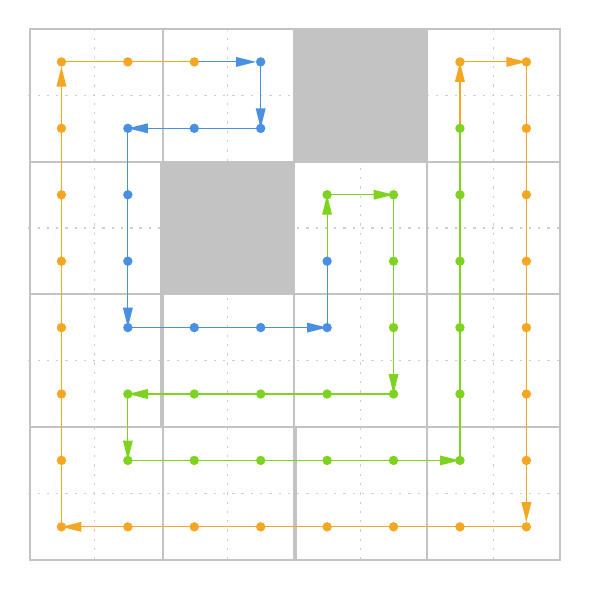
\begin{tikzpicture}[x=0.75pt,y=0.75pt,yscale=-0.8,xscale=0.8]
			%uncomment if require: \path (0,409); %set diagram left start at 0, and has height of 409
			
			%Straight Lines [id:da5351549802319371] 
			\draw [color={rgb, 255:red, 126; green, 211; blue, 33 }  ,draw opacity=1 ]   (351,195) -- (351,157) ;
			\draw [shift={(351,155)}, rotate = 450] [fill={rgb, 255:red, 126; green, 211; blue, 33 }  ,fill opacity=1 ][line width=0.08]  [draw opacity=0] (12,-3) -- (0,0) -- (12,3) -- cycle    ;
			%Straight Lines [id:da21302010090140722] 
			\draw [color={rgb, 255:red, 74; green, 144; blue, 226 }  ,draw opacity=1 ]   (271,75) -- (306.17,75) ;
			\draw [shift={(308.17,75)}, rotate = 180] [fill={rgb, 255:red, 74; green, 144; blue, 226 }  ,fill opacity=1 ][line width=0.08]  [draw opacity=0] (12,-3) -- (0,0) -- (12,3) -- cycle    ;
			%Straight Lines [id:da854517458794269] 
			\draw [color={rgb, 255:red, 195; green, 195; blue, 195 }  ,draw opacity=0.8 ] [dash pattern={on 0.84pt off 2.51pt}]  (211,55) -- (211,375) ;
			%Straight Lines [id:da5657085791005156] 
			\draw [color={rgb, 255:red, 195; green, 195; blue, 195 }  ,draw opacity=0.8 ] [dash pattern={on 0.84pt off 2.51pt}]  (291,55) -- (291,375) ;
			%Straight Lines [id:da2718901706564181] 
			\draw [color={rgb, 255:red, 195; green, 195; blue, 195 }  ,draw opacity=0.8 ] [dash pattern={on 0.84pt off 2.51pt}]  (371,55) -- (371,375) ;
			%Straight Lines [id:da02094912115129599] 
			\draw [color={rgb, 255:red, 195; green, 195; blue, 195 }  ,draw opacity=0.8 ] [dash pattern={on 0.84pt off 2.51pt}]  (451,55) -- (451,375) ;
			%Straight Lines [id:da9533932703135517] 
			\draw [color={rgb, 255:red, 195; green, 195; blue, 195 }  ,draw opacity=0.8 ] [dash pattern={on 0.84pt off 2.51pt}]  (171,95) -- (491,95) ;
			%Straight Lines [id:da9004292598975747] 
			\draw [color={rgb, 255:red, 195; green, 195; blue, 195 }  ,draw opacity=0.8 ] [dash pattern={on 0.84pt off 2.51pt}]  (171,175) -- (491,175) ;
			%Straight Lines [id:da1627688683660009] 
			\draw [color={rgb, 255:red, 195; green, 195; blue, 195 }  ,draw opacity=0.8 ] [dash pattern={on 0.84pt off 2.51pt}]  (171,255) -- (491,255) ;
			%Straight Lines [id:da4991285432755932] 
			\draw [color={rgb, 255:red, 195; green, 195; blue, 195 }  ,draw opacity=0.8 ] [dash pattern={on 0.84pt off 2.51pt}]  (171,335) -- (491,335) ;
			
			%Straight Lines [id:da7491713727663103] 
			\draw [color={rgb, 255:red, 245; green, 166; blue, 35 }  ,draw opacity=1 ]   (431,115) -- (431,77) ;
			\draw [shift={(431,75)}, rotate = 450] [fill={rgb, 255:red, 245; green, 166; blue, 35 }  ,fill opacity=1 ][line width=0.08]  [draw opacity=0] (12,-3) -- (0,0) -- (12,3) -- cycle    ;
			%Shape: Rectangle [id:dp8746081557149701] 
			\draw  [color={rgb, 255:red, 195; green, 195; blue, 195 }  ,draw opacity=1 ][line width=0.75]  (411,55) -- (491,55) -- (491,135) -- (411,135) -- cycle ;
			%Shape: Rectangle [id:dp04998372489748726] 
			\draw  [color={rgb, 255:red, 195; green, 195; blue, 195 }  ,draw opacity=1 ][line width=0.75]  (411,135) -- (491,135) -- (491,215) -- (411,215) -- cycle ;
			%Shape: Rectangle [id:dp716343211155213] 
			\draw  [color={rgb, 255:red, 195; green, 195; blue, 195 }  ,draw opacity=1 ][line width=0.75]  (411,215) -- (491,215) -- (491,295) -- (411,295) -- cycle ;
			%Shape: Rectangle [id:dp9628316526459462] 
			\draw  [color={rgb, 255:red, 195; green, 195; blue, 195 }  ,draw opacity=1 ][line width=0.75]  (411,295) -- (491,295) -- (491,375) -- (411,375) -- cycle ;
			%Shape: Rectangle [id:dp664440026053819] 
			\draw  [color={rgb, 255:red, 195; green, 195; blue, 195 }  ,draw opacity=1 ][line width=0.75]  (331,135) -- (411,135) -- (411,215) -- (331,215) -- cycle ;
			%Shape: Rectangle [id:dp08410695657353351] 
			\draw  [color={rgb, 255:red, 195; green, 195; blue, 195 }  ,draw opacity=1 ][line width=0.75]  (331,215) -- (411,215) -- (411,295) -- (331,295) -- cycle ;
			%Shape: Rectangle [id:dp07090445501331866] 
			\draw  [color={rgb, 255:red, 195; green, 195; blue, 195 }  ,draw opacity=1 ][line width=0.75]  (331,295) -- (411,295) -- (411,375) -- (331,375) -- cycle ;
			%Shape: Rectangle [id:dp8696408090436851] 
			\draw  [color={rgb, 255:red, 195; green, 195; blue, 195 }  ,draw opacity=1 ][line width=0.75]  (252,55) -- (332,55) -- (332,135) -- (252,135) -- cycle ;
			%Shape: Rectangle [id:dp4746238836207364] 
			\draw  [color={rgb, 255:red, 195; green, 195; blue, 195 }  ,draw opacity=1 ][line width=0.75]  (172,55) -- (252,55) -- (252,135) -- (172,135) -- cycle ;
			%Shape: Rectangle [id:dp8657981727821324] 
			\draw  [color={rgb, 255:red, 195; green, 195; blue, 195 }  ,draw opacity=1 ][line width=0.75]  (172,135) -- (252,135) -- (252,215) -- (172,215) -- cycle ;
			%Shape: Rectangle [id:dp20551199499502526] 
			\draw  [color={rgb, 255:red, 195; green, 195; blue, 195 }  ,draw opacity=1 ][line width=0.75]  (172,215) -- (252,215) -- (252,295) -- (172,295) -- cycle ;
			%Shape: Rectangle [id:dp5033014313679982] 
			\draw  [color={rgb, 255:red, 195; green, 195; blue, 195 }  ,draw opacity=1 ][line width=0.75]  (172,295) -- (252,295) -- (252,375) -- (172,375) -- cycle ;
			%Shape: Rectangle [id:dp0691160736423535] 
			\draw  [color={rgb, 255:red, 195; green, 195; blue, 195 }  ,draw opacity=1 ][line width=0.75]  (251,215) -- (331,215) -- (331,295) -- (251,295) -- cycle ;
			%Shape: Rectangle [id:dp9673109533181607] 
			\draw  [color={rgb, 255:red, 195; green, 195; blue, 195 }  ,draw opacity=1 ][line width=0.75]  (252,295) -- (332,295) -- (332,375) -- (252,375) -- cycle ;
			
			%Shape: Rectangle [id:dp24113727014203779] 
			\draw  [color={rgb, 255:red, 195; green, 195; blue, 195 }  ,draw opacity=1 ][fill={rgb, 255:red, 195; green, 195; blue, 195 }  ,fill opacity=1 ][line width=0.75]  (331,55) -- (411,55) -- (411,135) -- (331,135) -- cycle ;
			%Shape: Rectangle [id:dp6453850559631755] 
			\draw  [color={rgb, 255:red, 195; green, 195; blue, 195 }  ,draw opacity=1 ][fill={rgb, 255:red, 195; green, 195; blue, 195 }  ,fill opacity=1 ][line width=0.75]  (251,135) -- (331,135) -- (331,215) -- (251,215) -- cycle ;
			%Shape: Circle [id:dp6801416953242614] 
			\draw  [draw opacity=0][fill={rgb, 255:red, 245; green, 166; blue, 35 }  ,fill opacity=1 ] (468.17,75) .. controls (468.17,73.43) and (469.43,72.17) .. (471,72.17) .. controls (472.57,72.17) and (473.83,73.43) .. (473.83,75) .. controls (473.83,76.57) and (472.57,77.83) .. (471,77.83) .. controls (469.43,77.83) and (468.17,76.57) .. (468.17,75) -- cycle ;
			%Shape: Circle [id:dp4604608393759837] 
			\draw  [draw opacity=0][fill={rgb, 255:red, 245; green, 166; blue, 35 }  ,fill opacity=1 ] (428.17,75) .. controls (428.17,73.43) and (429.43,72.17) .. (431,72.17) .. controls (432.57,72.17) and (433.83,73.43) .. (433.83,75) .. controls (433.83,76.57) and (432.57,77.83) .. (431,77.83) .. controls (429.43,77.83) and (428.17,76.57) .. (428.17,75) -- cycle ;
			%Shape: Circle [id:dp13822592778240006] 
			\draw  [draw opacity=0][fill={rgb, 255:red, 245; green, 166; blue, 35 }  ,fill opacity=1 ] (468.17,115) .. controls (468.17,113.43) and (469.43,112.17) .. (471,112.17) .. controls (472.57,112.17) and (473.83,113.43) .. (473.83,115) .. controls (473.83,116.57) and (472.57,117.83) .. (471,117.83) .. controls (469.43,117.83) and (468.17,116.57) .. (468.17,115) -- cycle ;
			%Shape: Circle [id:dp544207653797784] 
			\draw  [draw opacity=0][fill={rgb, 255:red, 245; green, 166; blue, 35 }  ,fill opacity=1 ] (468.17,155) .. controls (468.17,153.43) and (469.43,152.17) .. (471,152.17) .. controls (472.57,152.17) and (473.83,153.43) .. (473.83,155) .. controls (473.83,156.57) and (472.57,157.83) .. (471,157.83) .. controls (469.43,157.83) and (468.17,156.57) .. (468.17,155) -- cycle ;
			%Shape: Circle [id:dp4171778626191891] 
			\draw  [draw opacity=0][fill={rgb, 255:red, 245; green, 166; blue, 35 }  ,fill opacity=1 ] (468.17,195) .. controls (468.17,193.43) and (469.43,192.17) .. (471,192.17) .. controls (472.57,192.17) and (473.83,193.43) .. (473.83,195) .. controls (473.83,196.57) and (472.57,197.83) .. (471,197.83) .. controls (469.43,197.83) and (468.17,196.57) .. (468.17,195) -- cycle ;
			%Shape: Circle [id:dp7895311637274933] 
			\draw  [draw opacity=0][fill={rgb, 255:red, 245; green, 166; blue, 35 }  ,fill opacity=1 ] (468.17,235) .. controls (468.17,233.43) and (469.43,232.17) .. (471,232.17) .. controls (472.57,232.17) and (473.83,233.43) .. (473.83,235) .. controls (473.83,236.57) and (472.57,237.83) .. (471,237.83) .. controls (469.43,237.83) and (468.17,236.57) .. (468.17,235) -- cycle ;
			%Shape: Circle [id:dp16643331735014688] 
			\draw  [draw opacity=0][fill={rgb, 255:red, 245; green, 166; blue, 35 }  ,fill opacity=1 ] (468.17,275) .. controls (468.17,273.43) and (469.43,272.17) .. (471,272.17) .. controls (472.57,272.17) and (473.83,273.43) .. (473.83,275) .. controls (473.83,276.57) and (472.57,277.83) .. (471,277.83) .. controls (469.43,277.83) and (468.17,276.57) .. (468.17,275) -- cycle ;
			%Shape: Circle [id:dp4612402233444193] 
			\draw  [draw opacity=0][fill={rgb, 255:red, 245; green, 166; blue, 35 }  ,fill opacity=1 ] (468.17,315) .. controls (468.17,313.43) and (469.43,312.17) .. (471,312.17) .. controls (472.57,312.17) and (473.83,313.43) .. (473.83,315) .. controls (473.83,316.57) and (472.57,317.83) .. (471,317.83) .. controls (469.43,317.83) and (468.17,316.57) .. (468.17,315) -- cycle ;
			%Shape: Circle [id:dp10168213951386096] 
			\draw  [draw opacity=0][fill={rgb, 255:red, 245; green, 166; blue, 35 }  ,fill opacity=1 ] (468.17,355) .. controls (468.17,353.43) and (469.43,352.17) .. (471,352.17) .. controls (472.57,352.17) and (473.83,353.43) .. (473.83,355) .. controls (473.83,356.57) and (472.57,357.83) .. (471,357.83) .. controls (469.43,357.83) and (468.17,356.57) .. (468.17,355) -- cycle ;
			%Shape: Circle [id:dp16583621916165892] 
			\draw  [draw opacity=0][fill={rgb, 255:red, 245; green, 166; blue, 35 }  ,fill opacity=1 ] (428.17,355) .. controls (428.17,353.43) and (429.43,352.17) .. (431,352.17) .. controls (432.57,352.17) and (433.83,353.43) .. (433.83,355) .. controls (433.83,356.57) and (432.57,357.83) .. (431,357.83) .. controls (429.43,357.83) and (428.17,356.57) .. (428.17,355) -- cycle ;
			%Shape: Circle [id:dp23056644975317875] 
			\draw  [draw opacity=0][fill={rgb, 255:red, 245; green, 166; blue, 35 }  ,fill opacity=1 ] (388.17,355) .. controls (388.17,353.43) and (389.43,352.17) .. (391,352.17) .. controls (392.57,352.17) and (393.83,353.43) .. (393.83,355) .. controls (393.83,356.57) and (392.57,357.83) .. (391,357.83) .. controls (389.43,357.83) and (388.17,356.57) .. (388.17,355) -- cycle ;
			%Shape: Circle [id:dp8401836553855346] 
			\draw  [draw opacity=0][fill={rgb, 255:red, 245; green, 166; blue, 35 }  ,fill opacity=1 ] (348.17,355) .. controls (348.17,353.43) and (349.43,352.17) .. (351,352.17) .. controls (352.57,352.17) and (353.83,353.43) .. (353.83,355) .. controls (353.83,356.57) and (352.57,357.83) .. (351,357.83) .. controls (349.43,357.83) and (348.17,356.57) .. (348.17,355) -- cycle ;
			%Shape: Circle [id:dp48282190307261685] 
			\draw  [draw opacity=0][fill={rgb, 255:red, 245; green, 166; blue, 35 }  ,fill opacity=1 ] (308.17,355) .. controls (308.17,353.43) and (309.43,352.17) .. (311,352.17) .. controls (312.57,352.17) and (313.83,353.43) .. (313.83,355) .. controls (313.83,356.57) and (312.57,357.83) .. (311,357.83) .. controls (309.43,357.83) and (308.17,356.57) .. (308.17,355) -- cycle ;
			%Shape: Circle [id:dp5761975450405177] 
			\draw  [draw opacity=0][fill={rgb, 255:red, 245; green, 166; blue, 35 }  ,fill opacity=1 ] (268.17,355) .. controls (268.17,353.43) and (269.43,352.17) .. (271,352.17) .. controls (272.57,352.17) and (273.83,353.43) .. (273.83,355) .. controls (273.83,356.57) and (272.57,357.83) .. (271,357.83) .. controls (269.43,357.83) and (268.17,356.57) .. (268.17,355) -- cycle ;
			%Shape: Circle [id:dp06870423995803909] 
			\draw  [draw opacity=0][fill={rgb, 255:red, 245; green, 166; blue, 35 }  ,fill opacity=1 ] (228.17,355) .. controls (228.17,353.43) and (229.43,352.17) .. (231,352.17) .. controls (232.57,352.17) and (233.83,353.43) .. (233.83,355) .. controls (233.83,356.57) and (232.57,357.83) .. (231,357.83) .. controls (229.43,357.83) and (228.17,356.57) .. (228.17,355) -- cycle ;
			%Shape: Circle [id:dp5381906142714585] 
			\draw  [draw opacity=0][fill={rgb, 255:red, 245; green, 166; blue, 35 }  ,fill opacity=1 ] (188.17,355) .. controls (188.17,353.43) and (189.43,352.17) .. (191,352.17) .. controls (192.57,352.17) and (193.83,353.43) .. (193.83,355) .. controls (193.83,356.57) and (192.57,357.83) .. (191,357.83) .. controls (189.43,357.83) and (188.17,356.57) .. (188.17,355) -- cycle ;
			%Shape: Circle [id:dp03637900283495887] 
			\draw  [draw opacity=0][fill={rgb, 255:red, 245; green, 166; blue, 35 }  ,fill opacity=1 ] (188.17,315) .. controls (188.17,313.43) and (189.43,312.17) .. (191,312.17) .. controls (192.57,312.17) and (193.83,313.43) .. (193.83,315) .. controls (193.83,316.57) and (192.57,317.83) .. (191,317.83) .. controls (189.43,317.83) and (188.17,316.57) .. (188.17,315) -- cycle ;
			%Shape: Circle [id:dp5512808090993917] 
			\draw  [draw opacity=0][fill={rgb, 255:red, 245; green, 166; blue, 35 }  ,fill opacity=1 ] (188.17,275) .. controls (188.17,273.43) and (189.43,272.17) .. (191,272.17) .. controls (192.57,272.17) and (193.83,273.43) .. (193.83,275) .. controls (193.83,276.57) and (192.57,277.83) .. (191,277.83) .. controls (189.43,277.83) and (188.17,276.57) .. (188.17,275) -- cycle ;
			%Shape: Circle [id:dp7146308141223112] 
			\draw  [draw opacity=0][fill={rgb, 255:red, 245; green, 166; blue, 35 }  ,fill opacity=1 ] (188.17,235) .. controls (188.17,233.43) and (189.43,232.17) .. (191,232.17) .. controls (192.57,232.17) and (193.83,233.43) .. (193.83,235) .. controls (193.83,236.57) and (192.57,237.83) .. (191,237.83) .. controls (189.43,237.83) and (188.17,236.57) .. (188.17,235) -- cycle ;
			%Shape: Circle [id:dp5335478422961473] 
			\draw  [draw opacity=0][fill={rgb, 255:red, 245; green, 166; blue, 35 }  ,fill opacity=1 ] (188.17,195) .. controls (188.17,193.43) and (189.43,192.17) .. (191,192.17) .. controls (192.57,192.17) and (193.83,193.43) .. (193.83,195) .. controls (193.83,196.57) and (192.57,197.83) .. (191,197.83) .. controls (189.43,197.83) and (188.17,196.57) .. (188.17,195) -- cycle ;
			%Shape: Circle [id:dp8716915789137862] 
			\draw  [draw opacity=0][fill={rgb, 255:red, 245; green, 166; blue, 35 }  ,fill opacity=1 ] (188.17,155) .. controls (188.17,153.43) and (189.43,152.17) .. (191,152.17) .. controls (192.57,152.17) and (193.83,153.43) .. (193.83,155) .. controls (193.83,156.57) and (192.57,157.83) .. (191,157.83) .. controls (189.43,157.83) and (188.17,156.57) .. (188.17,155) -- cycle ;
			%Shape: Circle [id:dp3349585094431857] 
			\draw  [draw opacity=0][fill={rgb, 255:red, 245; green, 166; blue, 35 }  ,fill opacity=1 ] (188.17,115) .. controls (188.17,113.43) and (189.43,112.17) .. (191,112.17) .. controls (192.57,112.17) and (193.83,113.43) .. (193.83,115) .. controls (193.83,116.57) and (192.57,117.83) .. (191,117.83) .. controls (189.43,117.83) and (188.17,116.57) .. (188.17,115) -- cycle ;
			%Shape: Circle [id:dp44273518739120976] 
			\draw  [draw opacity=0][fill={rgb, 255:red, 245; green, 166; blue, 35 }  ,fill opacity=1 ] (188.17,75) .. controls (188.17,73.43) and (189.43,72.17) .. (191,72.17) .. controls (192.57,72.17) and (193.83,73.43) .. (193.83,75) .. controls (193.83,76.57) and (192.57,77.83) .. (191,77.83) .. controls (189.43,77.83) and (188.17,76.57) .. (188.17,75) -- cycle ;
			%Shape: Circle [id:dp8508549485124735] 
			\draw  [draw opacity=0][fill={rgb, 255:red, 245; green, 166; blue, 35 }  ,fill opacity=1 ] (228.17,75) .. controls (228.17,73.43) and (229.43,72.17) .. (231,72.17) .. controls (232.57,72.17) and (233.83,73.43) .. (233.83,75) .. controls (233.83,76.57) and (232.57,77.83) .. (231,77.83) .. controls (229.43,77.83) and (228.17,76.57) .. (228.17,75) -- cycle ;
			%Shape: Circle [id:dp6783308931260619] 
			\draw  [draw opacity=0][fill={rgb, 255:red, 245; green, 166; blue, 35 }  ,fill opacity=1 ] (268.17,75) .. controls (268.17,73.43) and (269.43,72.17) .. (271,72.17) .. controls (272.57,72.17) and (273.83,73.43) .. (273.83,75) .. controls (273.83,76.57) and (272.57,77.83) .. (271,77.83) .. controls (269.43,77.83) and (268.17,76.57) .. (268.17,75) -- cycle ;
			%Straight Lines [id:da5456587577326129] 
			\draw [color={rgb, 255:red, 245; green, 166; blue, 35 }  ,draw opacity=1 ]   (431,75) -- (469,75) ;
			\draw [shift={(471,75)}, rotate = 180] [fill={rgb, 255:red, 245; green, 166; blue, 35 }  ,fill opacity=1 ][line width=0.08]  [draw opacity=0] (12,-3) -- (0,0) -- (12,3) -- cycle    ;
			%Shape: Circle [id:dp4443238058444041] 
			\draw  [draw opacity=0][fill={rgb, 255:red, 74; green, 144; blue, 226 }  ,fill opacity=1 ] (308.17,75) .. controls (308.17,73.43) and (309.43,72.17) .. (311,72.17) .. controls (312.57,72.17) and (313.83,73.43) .. (313.83,75) .. controls (313.83,76.57) and (312.57,77.83) .. (311,77.83) .. controls (309.43,77.83) and (308.17,76.57) .. (308.17,75) -- cycle ;
			%Shape: Circle [id:dp29010302295723345] 
			\draw  [draw opacity=0][fill={rgb, 255:red, 74; green, 144; blue, 226 }  ,fill opacity=1 ] (308.17,115) .. controls (308.17,113.43) and (309.43,112.17) .. (311,112.17) .. controls (312.57,112.17) and (313.83,113.43) .. (313.83,115) .. controls (313.83,116.57) and (312.57,117.83) .. (311,117.83) .. controls (309.43,117.83) and (308.17,116.57) .. (308.17,115) -- cycle ;
			%Shape: Circle [id:dp6216098523896874] 
			\draw  [draw opacity=0][fill={rgb, 255:red, 74; green, 144; blue, 226 }  ,fill opacity=1 ] (268.17,115) .. controls (268.17,113.43) and (269.43,112.17) .. (271,112.17) .. controls (272.57,112.17) and (273.83,113.43) .. (273.83,115) .. controls (273.83,116.57) and (272.57,117.83) .. (271,117.83) .. controls (269.43,117.83) and (268.17,116.57) .. (268.17,115) -- cycle ;
			%Shape: Circle [id:dp06234830362754895] 
			\draw  [draw opacity=0][fill={rgb, 255:red, 74; green, 144; blue, 226 }  ,fill opacity=1 ] (228.17,115) .. controls (228.17,113.43) and (229.43,112.17) .. (231,112.17) .. controls (232.57,112.17) and (233.83,113.43) .. (233.83,115) .. controls (233.83,116.57) and (232.57,117.83) .. (231,117.83) .. controls (229.43,117.83) and (228.17,116.57) .. (228.17,115) -- cycle ;
			%Shape: Circle [id:dp9885173496004662] 
			\draw  [draw opacity=0][fill={rgb, 255:red, 74; green, 144; blue, 226 }  ,fill opacity=1 ] (228.17,155) .. controls (228.17,153.43) and (229.43,152.17) .. (231,152.17) .. controls (232.57,152.17) and (233.83,153.43) .. (233.83,155) .. controls (233.83,156.57) and (232.57,157.83) .. (231,157.83) .. controls (229.43,157.83) and (228.17,156.57) .. (228.17,155) -- cycle ;
			%Shape: Circle [id:dp9444674235776642] 
			\draw  [draw opacity=0][fill={rgb, 255:red, 74; green, 144; blue, 226 }  ,fill opacity=1 ] (228.17,195) .. controls (228.17,193.43) and (229.43,192.17) .. (231,192.17) .. controls (232.57,192.17) and (233.83,193.43) .. (233.83,195) .. controls (233.83,196.57) and (232.57,197.83) .. (231,197.83) .. controls (229.43,197.83) and (228.17,196.57) .. (228.17,195) -- cycle ;
			%Shape: Circle [id:dp7868027408873275] 
			\draw  [draw opacity=0][fill={rgb, 255:red, 74; green, 144; blue, 226 }  ,fill opacity=1 ] (228.17,235) .. controls (228.17,233.43) and (229.43,232.17) .. (231,232.17) .. controls (232.57,232.17) and (233.83,233.43) .. (233.83,235) .. controls (233.83,236.57) and (232.57,237.83) .. (231,237.83) .. controls (229.43,237.83) and (228.17,236.57) .. (228.17,235) -- cycle ;
			%Shape: Circle [id:dp35955963628126275] 
			\draw  [draw opacity=0][fill={rgb, 255:red, 74; green, 144; blue, 226 }  ,fill opacity=1 ] (268.17,235) .. controls (268.17,233.43) and (269.43,232.17) .. (271,232.17) .. controls (272.57,232.17) and (273.83,233.43) .. (273.83,235) .. controls (273.83,236.57) and (272.57,237.83) .. (271,237.83) .. controls (269.43,237.83) and (268.17,236.57) .. (268.17,235) -- cycle ;
			%Shape: Circle [id:dp5516376120857398] 
			\draw  [draw opacity=0][fill={rgb, 255:red, 74; green, 144; blue, 226 }  ,fill opacity=1 ] (308.17,235) .. controls (308.17,233.43) and (309.43,232.17) .. (311,232.17) .. controls (312.57,232.17) and (313.83,233.43) .. (313.83,235) .. controls (313.83,236.57) and (312.57,237.83) .. (311,237.83) .. controls (309.43,237.83) and (308.17,236.57) .. (308.17,235) -- cycle ;
			%Shape: Circle [id:dp5893700740487555] 
			\draw  [draw opacity=0][fill={rgb, 255:red, 74; green, 144; blue, 226 }  ,fill opacity=1 ] (348.17,235) .. controls (348.17,233.43) and (349.43,232.17) .. (351,232.17) .. controls (352.57,232.17) and (353.83,233.43) .. (353.83,235) .. controls (353.83,236.57) and (352.57,237.83) .. (351,237.83) .. controls (349.43,237.83) and (348.17,236.57) .. (348.17,235) -- cycle ;
			%Shape: Circle [id:dp1286587461477784] 
			\draw  [draw opacity=0][fill={rgb, 255:red, 74; green, 144; blue, 226 }  ,fill opacity=1 ] (348.17,195) .. controls (348.17,193.43) and (349.43,192.17) .. (351,192.17) .. controls (352.57,192.17) and (353.83,193.43) .. (353.83,195) .. controls (353.83,196.57) and (352.57,197.83) .. (351,197.83) .. controls (349.43,197.83) and (348.17,196.57) .. (348.17,195) -- cycle ;
			%Shape: Circle [id:dp26088941378322006] 
			\draw  [draw opacity=0][fill={rgb, 255:red, 126; green, 211; blue, 33 }  ,fill opacity=1 ] (348.17,155) .. controls (348.17,153.43) and (349.43,152.17) .. (351,152.17) .. controls (352.57,152.17) and (353.83,153.43) .. (353.83,155) .. controls (353.83,156.57) and (352.57,157.83) .. (351,157.83) .. controls (349.43,157.83) and (348.17,156.57) .. (348.17,155) -- cycle ;
			%Shape: Circle [id:dp9676514649936712] 
			\draw  [draw opacity=0][fill={rgb, 255:red, 126; green, 211; blue, 33 }  ,fill opacity=1 ] (388.17,155) .. controls (388.17,153.43) and (389.43,152.17) .. (391,152.17) .. controls (392.57,152.17) and (393.83,153.43) .. (393.83,155) .. controls (393.83,156.57) and (392.57,157.83) .. (391,157.83) .. controls (389.43,157.83) and (388.17,156.57) .. (388.17,155) -- cycle ;
			%Shape: Circle [id:dp19213789582339302] 
			\draw  [draw opacity=0][fill={rgb, 255:red, 126; green, 211; blue, 33 }  ,fill opacity=1 ] (388.17,195) .. controls (388.17,193.43) and (389.43,192.17) .. (391,192.17) .. controls (392.57,192.17) and (393.83,193.43) .. (393.83,195) .. controls (393.83,196.57) and (392.57,197.83) .. (391,197.83) .. controls (389.43,197.83) and (388.17,196.57) .. (388.17,195) -- cycle ;
			%Shape: Circle [id:dp31757377829209155] 
			\draw  [draw opacity=0][fill={rgb, 255:red, 126; green, 211; blue, 33 }  ,fill opacity=1 ] (388.17,235) .. controls (388.17,233.43) and (389.43,232.17) .. (391,232.17) .. controls (392.57,232.17) and (393.83,233.43) .. (393.83,235) .. controls (393.83,236.57) and (392.57,237.83) .. (391,237.83) .. controls (389.43,237.83) and (388.17,236.57) .. (388.17,235) -- cycle ;
			%Shape: Circle [id:dp11411146161431085] 
			\draw  [draw opacity=0][fill={rgb, 255:red, 126; green, 211; blue, 33 }  ,fill opacity=1 ] (388.17,275) .. controls (388.17,273.43) and (389.43,272.17) .. (391,272.17) .. controls (392.57,272.17) and (393.83,273.43) .. (393.83,275) .. controls (393.83,276.57) and (392.57,277.83) .. (391,277.83) .. controls (389.43,277.83) and (388.17,276.57) .. (388.17,275) -- cycle ;
			%Shape: Circle [id:dp6075376860133745] 
			\draw  [draw opacity=0][fill={rgb, 255:red, 126; green, 211; blue, 33 }  ,fill opacity=1 ] (348.17,275) .. controls (348.17,273.43) and (349.43,272.17) .. (351,272.17) .. controls (352.57,272.17) and (353.83,273.43) .. (353.83,275) .. controls (353.83,276.57) and (352.57,277.83) .. (351,277.83) .. controls (349.43,277.83) and (348.17,276.57) .. (348.17,275) -- cycle ;
			%Shape: Circle [id:dp33787943985666535] 
			\draw  [draw opacity=0][fill={rgb, 255:red, 126; green, 211; blue, 33 }  ,fill opacity=1 ] (308.17,275) .. controls (308.17,273.43) and (309.43,272.17) .. (311,272.17) .. controls (312.57,272.17) and (313.83,273.43) .. (313.83,275) .. controls (313.83,276.57) and (312.57,277.83) .. (311,277.83) .. controls (309.43,277.83) and (308.17,276.57) .. (308.17,275) -- cycle ;
			%Shape: Circle [id:dp6967659869352532] 
			\draw  [draw opacity=0][fill={rgb, 255:red, 126; green, 211; blue, 33 }  ,fill opacity=1 ] (268.17,275) .. controls (268.17,273.43) and (269.43,272.17) .. (271,272.17) .. controls (272.57,272.17) and (273.83,273.43) .. (273.83,275) .. controls (273.83,276.57) and (272.57,277.83) .. (271,277.83) .. controls (269.43,277.83) and (268.17,276.57) .. (268.17,275) -- cycle ;
			%Shape: Circle [id:dp7916368779271419] 
			\draw  [draw opacity=0][fill={rgb, 255:red, 126; green, 211; blue, 33 }  ,fill opacity=1 ] (228.17,275) .. controls (228.17,273.43) and (229.43,272.17) .. (231,272.17) .. controls (232.57,272.17) and (233.83,273.43) .. (233.83,275) .. controls (233.83,276.57) and (232.57,277.83) .. (231,277.83) .. controls (229.43,277.83) and (228.17,276.57) .. (228.17,275) -- cycle ;
			%Shape: Circle [id:dp9131057577477717] 
			\draw  [draw opacity=0][fill={rgb, 255:red, 126; green, 211; blue, 33 }  ,fill opacity=1 ] (228.17,315) .. controls (228.17,313.43) and (229.43,312.17) .. (231,312.17) .. controls (232.57,312.17) and (233.83,313.43) .. (233.83,315) .. controls (233.83,316.57) and (232.57,317.83) .. (231,317.83) .. controls (229.43,317.83) and (228.17,316.57) .. (228.17,315) -- cycle ;
			%Shape: Circle [id:dp060540910098607625] 
			\draw  [draw opacity=0][fill={rgb, 255:red, 126; green, 211; blue, 33 }  ,fill opacity=1 ] (268.17,315) .. controls (268.17,313.43) and (269.43,312.17) .. (271,312.17) .. controls (272.57,312.17) and (273.83,313.43) .. (273.83,315) .. controls (273.83,316.57) and (272.57,317.83) .. (271,317.83) .. controls (269.43,317.83) and (268.17,316.57) .. (268.17,315) -- cycle ;
			%Shape: Circle [id:dp4358067111786901] 
			\draw  [draw opacity=0][fill={rgb, 255:red, 126; green, 211; blue, 33 }  ,fill opacity=1 ] (308.17,315) .. controls (308.17,313.43) and (309.43,312.17) .. (311,312.17) .. controls (312.57,312.17) and (313.83,313.43) .. (313.83,315) .. controls (313.83,316.57) and (312.57,317.83) .. (311,317.83) .. controls (309.43,317.83) and (308.17,316.57) .. (308.17,315) -- cycle ;
			%Shape: Circle [id:dp6562545880538291] 
			\draw  [draw opacity=0][fill={rgb, 255:red, 126; green, 211; blue, 33 }  ,fill opacity=1 ] (348.17,315) .. controls (348.17,313.43) and (349.43,312.17) .. (351,312.17) .. controls (352.57,312.17) and (353.83,313.43) .. (353.83,315) .. controls (353.83,316.57) and (352.57,317.83) .. (351,317.83) .. controls (349.43,317.83) and (348.17,316.57) .. (348.17,315) -- cycle ;
			%Shape: Circle [id:dp18058415370378111] 
			\draw  [draw opacity=0][fill={rgb, 255:red, 126; green, 211; blue, 33 }  ,fill opacity=1 ] (388.17,315) .. controls (388.17,313.43) and (389.43,312.17) .. (391,312.17) .. controls (392.57,312.17) and (393.83,313.43) .. (393.83,315) .. controls (393.83,316.57) and (392.57,317.83) .. (391,317.83) .. controls (389.43,317.83) and (388.17,316.57) .. (388.17,315) -- cycle ;
			%Shape: Circle [id:dp10115316904907612] 
			\draw  [draw opacity=0][fill={rgb, 255:red, 126; green, 211; blue, 33 }  ,fill opacity=1 ] (428.17,315) .. controls (428.17,313.43) and (429.43,312.17) .. (431,312.17) .. controls (432.57,312.17) and (433.83,313.43) .. (433.83,315) .. controls (433.83,316.57) and (432.57,317.83) .. (431,317.83) .. controls (429.43,317.83) and (428.17,316.57) .. (428.17,315) -- cycle ;
			%Shape: Circle [id:dp835742083306757] 
			\draw  [draw opacity=0][fill={rgb, 255:red, 126; green, 211; blue, 33 }  ,fill opacity=1 ] (428.17,275) .. controls (428.17,273.43) and (429.43,272.17) .. (431,272.17) .. controls (432.57,272.17) and (433.83,273.43) .. (433.83,275) .. controls (433.83,276.57) and (432.57,277.83) .. (431,277.83) .. controls (429.43,277.83) and (428.17,276.57) .. (428.17,275) -- cycle ;
			%Shape: Circle [id:dp780791295796917] 
			\draw  [draw opacity=0][fill={rgb, 255:red, 126; green, 211; blue, 33 }  ,fill opacity=1 ] (428.17,235) .. controls (428.17,233.43) and (429.43,232.17) .. (431,232.17) .. controls (432.57,232.17) and (433.83,233.43) .. (433.83,235) .. controls (433.83,236.57) and (432.57,237.83) .. (431,237.83) .. controls (429.43,237.83) and (428.17,236.57) .. (428.17,235) -- cycle ;
			%Shape: Circle [id:dp742197015069753] 
			\draw  [draw opacity=0][fill={rgb, 255:red, 126; green, 211; blue, 33 }  ,fill opacity=1 ] (428.17,195) .. controls (428.17,193.43) and (429.43,192.17) .. (431,192.17) .. controls (432.57,192.17) and (433.83,193.43) .. (433.83,195) .. controls (433.83,196.57) and (432.57,197.83) .. (431,197.83) .. controls (429.43,197.83) and (428.17,196.57) .. (428.17,195) -- cycle ;
			%Shape: Circle [id:dp058172723888363365] 
			\draw  [draw opacity=0][fill={rgb, 255:red, 126; green, 211; blue, 33 }  ,fill opacity=1 ] (428.17,155) .. controls (428.17,153.43) and (429.43,152.17) .. (431,152.17) .. controls (432.57,152.17) and (433.83,153.43) .. (433.83,155) .. controls (433.83,156.57) and (432.57,157.83) .. (431,157.83) .. controls (429.43,157.83) and (428.17,156.57) .. (428.17,155) -- cycle ;
			%Shape: Circle [id:dp40603445670354055] 
			\draw  [draw opacity=0][fill={rgb, 255:red, 126; green, 211; blue, 33 }  ,fill opacity=1 ] (428.17,115) .. controls (428.17,113.43) and (429.43,112.17) .. (431,112.17) .. controls (432.57,112.17) and (433.83,113.43) .. (433.83,115) .. controls (433.83,116.57) and (432.57,117.83) .. (431,117.83) .. controls (429.43,117.83) and (428.17,116.57) .. (428.17,115) -- cycle ;
			%Straight Lines [id:da16789636771970073] 
			\draw [color={rgb, 255:red, 245; green, 166; blue, 35 }  ,draw opacity=1 ]   (471,75) -- (471,350.17) ;
			\draw [shift={(471,352.17)}, rotate = 270] [fill={rgb, 255:red, 245; green, 166; blue, 35 }  ,fill opacity=1 ][line width=0.08]  [draw opacity=0] (12,-3) -- (0,0) -- (12,3) -- cycle    ;
			%Straight Lines [id:da3449631876846895] 
			\draw [color={rgb, 255:red, 245; green, 166; blue, 35 }  ,draw opacity=1 ]   (471,355) -- (193,355) ;
			\draw [shift={(191,355)}, rotate = 360] [fill={rgb, 255:red, 245; green, 166; blue, 35 }  ,fill opacity=1 ][line width=0.08]  [draw opacity=0] (12,-3) -- (0,0) -- (12,3) -- cycle    ;
			%Straight Lines [id:da10161365475922346] 
			\draw [color={rgb, 255:red, 245; green, 166; blue, 35 }  ,draw opacity=1 ]   (191,355) -- (191,79.83) ;
			\draw [shift={(191,77.83)}, rotate = 450] [fill={rgb, 255:red, 245; green, 166; blue, 35 }  ,fill opacity=1 ][line width=0.08]  [draw opacity=0] (12,-3) -- (0,0) -- (12,3) -- cycle    ;
			%Straight Lines [id:da8632021686141709] 
			\draw [color={rgb, 255:red, 245; green, 166; blue, 35 }  ,draw opacity=1 ]   (191,75) -- (271,75) ;
			%Straight Lines [id:da7671632448461922] 
			\draw [color={rgb, 255:red, 74; green, 144; blue, 226 }  ,draw opacity=1 ]   (311,75) -- (311,113) ;
			\draw [shift={(311,115)}, rotate = 270] [fill={rgb, 255:red, 74; green, 144; blue, 226 }  ,fill opacity=1 ][line width=0.08]  [draw opacity=0] (12,-3) -- (0,0) -- (12,3) -- cycle    ;
			%Straight Lines [id:da672307594730295] 
			\draw [color={rgb, 255:red, 74; green, 144; blue, 226 }  ,draw opacity=1 ]   (311,115) -- (233,115) ;
			\draw [shift={(231,115)}, rotate = 360] [fill={rgb, 255:red, 74; green, 144; blue, 226 }  ,fill opacity=1 ][line width=0.08]  [draw opacity=0] (12,-3) -- (0,0) -- (12,3) -- cycle    ;
			%Straight Lines [id:da4077834871044419] 
			\draw [color={rgb, 255:red, 74; green, 144; blue, 226 }  ,draw opacity=1 ]   (231,115) -- (231,233) ;
			\draw [shift={(231,235)}, rotate = 270] [fill={rgb, 255:red, 74; green, 144; blue, 226 }  ,fill opacity=1 ][line width=0.08]  [draw opacity=0] (12,-3) -- (0,0) -- (12,3) -- cycle    ;
			%Straight Lines [id:da9346944539277193] 
			\draw [color={rgb, 255:red, 74; green, 144; blue, 226 }  ,draw opacity=1 ]   (231,235) -- (349,235) ;
			\draw [shift={(351,235)}, rotate = 180] [fill={rgb, 255:red, 74; green, 144; blue, 226 }  ,fill opacity=1 ][line width=0.08]  [draw opacity=0] (12,-3) -- (0,0) -- (12,3) -- cycle    ;
			%Straight Lines [id:da6701207435426635] 
			\draw [color={rgb, 255:red, 74; green, 144; blue, 226 }  ,draw opacity=1 ]   (351,235) -- (351,195) ;
			%Straight Lines [id:da5501151214452311] 
			\draw [color={rgb, 255:red, 126; green, 211; blue, 33 }  ,draw opacity=1 ]   (351,155) -- (389,155) ;
			\draw [shift={(391,155)}, rotate = 180] [fill={rgb, 255:red, 126; green, 211; blue, 33 }  ,fill opacity=1 ][line width=0.08]  [draw opacity=0] (12,-3) -- (0,0) -- (12,3) -- cycle    ;
			%Straight Lines [id:da4311911132527191] 
			\draw [color={rgb, 255:red, 126; green, 211; blue, 33 }  ,draw opacity=1 ]   (391,155) -- (391,194) -- (391,273) ;
			\draw [shift={(391,275)}, rotate = 270] [fill={rgb, 255:red, 126; green, 211; blue, 33 }  ,fill opacity=1 ][line width=0.08]  [draw opacity=0] (12,-3) -- (0,0) -- (12,3) -- cycle    ;
			%Straight Lines [id:da5705388383279479] 
			\draw [color={rgb, 255:red, 126; green, 211; blue, 33 }  ,draw opacity=1 ]   (391,275) -- (233,275) ;
			\draw [shift={(231,275)}, rotate = 360] [fill={rgb, 255:red, 126; green, 211; blue, 33 }  ,fill opacity=1 ][line width=0.08]  [draw opacity=0] (12,-3) -- (0,0) -- (12,3) -- cycle    ;
			%Straight Lines [id:da21297417889995085] 
			\draw [color={rgb, 255:red, 126; green, 211; blue, 33 }  ,draw opacity=1 ]   (231,275) -- (231,313) ;
			\draw [shift={(231,315)}, rotate = 270] [fill={rgb, 255:red, 126; green, 211; blue, 33 }  ,fill opacity=1 ][line width=0.08]  [draw opacity=0] (12,-3) -- (0,0) -- (12,3) -- cycle    ;
			%Straight Lines [id:da22819451965736026] 
			\draw [color={rgb, 255:red, 126; green, 211; blue, 33 }  ,draw opacity=1 ]   (231,315) -- (429,315) ;
			\draw [shift={(431,315)}, rotate = 180] [fill={rgb, 255:red, 126; green, 211; blue, 33 }  ,fill opacity=1 ][line width=0.08]  [draw opacity=0] (12,-3) -- (0,0) -- (12,3) -- cycle    ;
			%Straight Lines [id:da7504973565926707] 
			\draw [color={rgb, 255:red, 126; green, 211; blue, 33 }  ,draw opacity=1 ]   (431,315) -- (431,115) ;
			
			
			
			
		\end{tikzpicture}
		\caption{Path generated by generating way-points from arrows}
		\label{fig:wpnts01}
	\end{subfigure}
	\hfill
	\begin{subfigure}{0.45\textwidth}
		\centering
		\tikzset{every picture/.style={line width=0.75pt}} %set default line width to 0.75pt        
		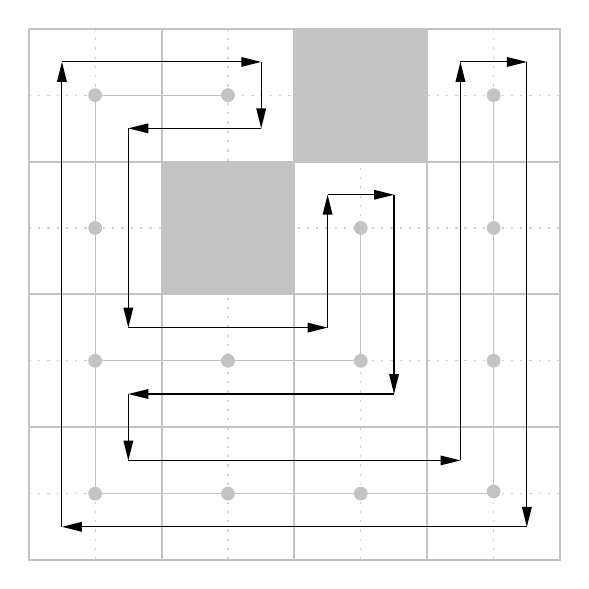
\begin{tikzpicture}[x=0.75pt,y=0.75pt,yscale=-0.8,xscale=0.8]
			%uncomment if require: \path (0,401); %set diagram left start at 0, and has height of 401
			
			%Straight Lines [id:da6525656097654802] 
			\draw [color={rgb, 255:red, 195; green, 195; blue, 195 }  ,draw opacity=0.8 ] [dash pattern={on 0.84pt off 2.51pt}]  (209,36) -- (209,356) ;
			%Straight Lines [id:da9449615822379405] 
			\draw [color={rgb, 255:red, 195; green, 195; blue, 195 }  ,draw opacity=0.8 ] [dash pattern={on 0.84pt off 2.51pt}]  (289,36) -- (289,356) ;
			%Straight Lines [id:da49922694692753367] 
			\draw [color={rgb, 255:red, 195; green, 195; blue, 195 }  ,draw opacity=0.8 ] [dash pattern={on 0.84pt off 2.51pt}]  (369,36) -- (369,356) ;
			%Straight Lines [id:da42403625075839124] 
			\draw [color={rgb, 255:red, 195; green, 195; blue, 195 }  ,draw opacity=0.8 ] [dash pattern={on 0.84pt off 2.51pt}]  (449,36) -- (449,356) ;
			%Straight Lines [id:da41382258883228107] 
			\draw [color={rgb, 255:red, 195; green, 195; blue, 195 }  ,draw opacity=0.8 ] [dash pattern={on 0.84pt off 2.51pt}]  (169,76) -- (489,76) ;
			%Straight Lines [id:da37487046166351323] 
			\draw [color={rgb, 255:red, 195; green, 195; blue, 195 }  ,draw opacity=0.8 ] [dash pattern={on 0.84pt off 2.51pt}]  (169,156) -- (489,156) ;
			%Straight Lines [id:da7805503540839331] 
			\draw [color={rgb, 255:red, 195; green, 195; blue, 195 }  ,draw opacity=0.8 ] [dash pattern={on 0.84pt off 2.51pt}]  (169,236) -- (489,236) ;
			%Straight Lines [id:da0007847063653105835] 
			\draw [color={rgb, 255:red, 195; green, 195; blue, 195 }  ,draw opacity=0.8 ] [dash pattern={on 0.84pt off 2.51pt}]  (169,316) -- (489,316) ;
			
			%Shape: Rectangle [id:dp9282250935920651] 
			\draw  [color={rgb, 255:red, 195; green, 195; blue, 195 }  ,draw opacity=1 ][line width=0.75]  (409,36) -- (489,36) -- (489,116) -- (409,116) -- cycle ;
			%Shape: Rectangle [id:dp40889920048446493] 
			\draw  [color={rgb, 255:red, 195; green, 195; blue, 195 }  ,draw opacity=1 ][line width=0.75]  (409,116) -- (489,116) -- (489,196) -- (409,196) -- cycle ;
			%Shape: Rectangle [id:dp08210856469103622] 
			\draw  [color={rgb, 255:red, 195; green, 195; blue, 195 }  ,draw opacity=1 ][line width=0.75]  (409,196) -- (489,196) -- (489,276) -- (409,276) -- cycle ;
			%Shape: Rectangle [id:dp11132018353927009] 
			\draw  [color={rgb, 255:red, 195; green, 195; blue, 195 }  ,draw opacity=1 ][line width=0.75]  (409,276) -- (489,276) -- (489,356) -- (409,356) -- cycle ;
			%Shape: Rectangle [id:dp056079390985070976] 
			\draw  [color={rgb, 255:red, 195; green, 195; blue, 195 }  ,draw opacity=1 ][line width=0.75]  (329,116) -- (409,116) -- (409,196) -- (329,196) -- cycle ;
			%Shape: Rectangle [id:dp8717884780085985] 
			\draw  [color={rgb, 255:red, 195; green, 195; blue, 195 }  ,draw opacity=1 ][line width=0.75]  (329,196) -- (409,196) -- (409,276) -- (329,276) -- cycle ;
			%Shape: Rectangle [id:dp6966702207831605] 
			\draw  [color={rgb, 255:red, 195; green, 195; blue, 195 }  ,draw opacity=1 ][line width=0.75]  (329,276) -- (409,276) -- (409,356) -- (329,356) -- cycle ;
			%Shape: Rectangle [id:dp6557240237758346] 
			\draw  [color={rgb, 255:red, 195; green, 195; blue, 195 }  ,draw opacity=1 ][line width=0.75]  (249,36) -- (329,36) -- (329,116) -- (249,116) -- cycle ;
			%Shape: Rectangle [id:dp46922355033620544] 
			\draw  [color={rgb, 255:red, 195; green, 195; blue, 195 }  ,draw opacity=1 ][line width=0.75]  (169,36) -- (249,36) -- (249,116) -- (169,116) -- cycle ;
			%Shape: Rectangle [id:dp7130641235448705] 
			\draw  [color={rgb, 255:red, 195; green, 195; blue, 195 }  ,draw opacity=1 ][line width=0.75]  (169,116) -- (249,116) -- (249,196) -- (169,196) -- cycle ;
			%Shape: Rectangle [id:dp8416366697669087] 
			\draw  [color={rgb, 255:red, 195; green, 195; blue, 195 }  ,draw opacity=1 ][line width=0.75]  (169,196) -- (249,196) -- (249,276) -- (169,276) -- cycle ;
			%Shape: Rectangle [id:dp5912644819544948] 
			\draw  [color={rgb, 255:red, 195; green, 195; blue, 195 }  ,draw opacity=1 ][line width=0.75]  (169,276) -- (249,276) -- (249,356) -- (169,356) -- cycle ;
			%Shape: Rectangle [id:dp6447358006368811] 
			\draw  [color={rgb, 255:red, 195; green, 195; blue, 195 }  ,draw opacity=1 ][line width=0.75]  (249,196) -- (329,196) -- (329,276) -- (249,276) -- cycle ;
			%Shape: Rectangle [id:dp8887506508423009] 
			\draw  [color={rgb, 255:red, 195; green, 195; blue, 195 }  ,draw opacity=1 ][line width=0.75]  (249,276) -- (329,276) -- (329,356) -- (249,356) -- cycle ;
			
			%Straight Lines [id:da1738948188181435] 
			\draw [color={rgb, 255:red, 195; green, 195; blue, 195 }  ,draw opacity=1 ]   (209,76) -- (265,76) -- (289,76) ;
			%Straight Lines [id:da7049505215325911] 
			\draw [color={rgb, 255:red, 195; green, 195; blue, 195 }  ,draw opacity=1 ]   (209,76) -- (209,316) ;
			%Straight Lines [id:da9869392385512394] 
			\draw [color={rgb, 255:red, 195; green, 195; blue, 195 }  ,draw opacity=1 ]   (209,316) -- (449,316) ;
			%Straight Lines [id:da1614981151805881] 
			\draw [color={rgb, 255:red, 195; green, 195; blue, 195 }  ,draw opacity=1 ]   (449,77) -- (449,317) ;
			%Straight Lines [id:da45917613825264225] 
			\draw [color={rgb, 255:red, 195; green, 195; blue, 195 }  ,draw opacity=1 ]   (369,237) -- (369,157) ;
			%Straight Lines [id:da6889780670091039] 
			\draw [color={rgb, 255:red, 195; green, 195; blue, 195 }  ,draw opacity=1 ]   (209,236) -- (369,236) ;
			%Straight Lines [id:da12273195124066882] 
			\draw [color={rgb, 255:red, 0; green, 0; blue, 0 }  ,draw opacity=1 ][fill={rgb, 255:red, 0; green, 0; blue, 0 }  ,fill opacity=1 ]   (349,216) -- (349,138) ;
			\draw [shift={(349,136)}, rotate = 450] [fill={rgb, 255:red, 0; green, 0; blue, 0 }  ,fill opacity=1 ][line width=0.08]  [draw opacity=0] (12,-3) -- (0,0) -- (12,3) -- cycle    ;
			%Straight Lines [id:da3917937162075191] 
			\draw [color={rgb, 255:red, 0; green, 0; blue, 0 }  ,draw opacity=1 ][fill={rgb, 255:red, 0; green, 0; blue, 0 }  ,fill opacity=1 ]   (229,216) -- (347,216) ;
			\draw [shift={(349,216)}, rotate = 180] [fill={rgb, 255:red, 0; green, 0; blue, 0 }  ,fill opacity=1 ][line width=0.08]  [draw opacity=0] (12,-3) -- (0,0) -- (12,3) -- cycle    ;
			%Straight Lines [id:da4803441771366592] 
			\draw [color={rgb, 255:red, 0; green, 0; blue, 0 }  ,draw opacity=1 ][fill={rgb, 255:red, 0; green, 0; blue, 0 }  ,fill opacity=1 ]   (229,96) -- (229,214) ;
			\draw [shift={(229,216)}, rotate = 270] [fill={rgb, 255:red, 0; green, 0; blue, 0 }  ,fill opacity=1 ][line width=0.08]  [draw opacity=0] (12,-3) -- (0,0) -- (12,3) -- cycle    ;
			%Straight Lines [id:da7402482792888903] 
			\draw [color={rgb, 255:red, 0; green, 0; blue, 0 }  ,draw opacity=1 ][fill={rgb, 255:red, 0; green, 0; blue, 0 }  ,fill opacity=1 ]   (309,96) -- (231,96) ;
			\draw [shift={(229,96)}, rotate = 360] [fill={rgb, 255:red, 0; green, 0; blue, 0 }  ,fill opacity=1 ][line width=0.08]  [draw opacity=0] (12,-3) -- (0,0) -- (12,3) -- cycle    ;
			%Straight Lines [id:da8948623102095223] 
			\draw [color={rgb, 255:red, 0; green, 0; blue, 0 }  ,draw opacity=1 ][fill={rgb, 255:red, 0; green, 0; blue, 0 }  ,fill opacity=1 ]   (309,56) -- (309,94) ;
			\draw [shift={(309,96)}, rotate = 270] [fill={rgb, 255:red, 0; green, 0; blue, 0 }  ,fill opacity=1 ][line width=0.08]  [draw opacity=0] (12,-3) -- (0,0) -- (12,3) -- cycle    ;
			%Straight Lines [id:da25998808169222265] 
			\draw [color={rgb, 255:red, 0; green, 0; blue, 0 }  ,draw opacity=1 ][fill={rgb, 255:red, 0; green, 0; blue, 0 }  ,fill opacity=1 ]   (189,56) -- (307,56) ;
			\draw [shift={(309,56)}, rotate = 180] [fill={rgb, 255:red, 0; green, 0; blue, 0 }  ,fill opacity=1 ][line width=0.08]  [draw opacity=0] (12,-3) -- (0,0) -- (12,3) -- cycle    ;
			%Straight Lines [id:da40263375664736256] 
			\draw [color={rgb, 255:red, 0; green, 0; blue, 0 }  ,draw opacity=1 ][fill={rgb, 255:red, 0; green, 0; blue, 0 }  ,fill opacity=1 ]   (189,336) -- (189,58) ;
			\draw [shift={(189,56)}, rotate = 450] [fill={rgb, 255:red, 0; green, 0; blue, 0 }  ,fill opacity=1 ][line width=0.08]  [draw opacity=0] (12,-3) -- (0,0) -- (12,3) -- cycle    ;
			%Straight Lines [id:da48570875534448854] 
			\draw [color={rgb, 255:red, 0; green, 0; blue, 0 }  ,draw opacity=1 ][fill={rgb, 255:red, 0; green, 0; blue, 0 }  ,fill opacity=1 ]   (469,336) -- (191,336) ;
			\draw [shift={(189,336)}, rotate = 360] [fill={rgb, 255:red, 0; green, 0; blue, 0 }  ,fill opacity=1 ][line width=0.08]  [draw opacity=0] (12,-3) -- (0,0) -- (12,3) -- cycle    ;
			%Straight Lines [id:da8647185294436568] 
			\draw [color={rgb, 255:red, 0; green, 0; blue, 0 }  ,draw opacity=1 ][fill={rgb, 255:red, 0; green, 0; blue, 0 }  ,fill opacity=1 ]   (469,56) -- (469,334) ;
			\draw [shift={(469,336)}, rotate = 270] [fill={rgb, 255:red, 0; green, 0; blue, 0 }  ,fill opacity=1 ][line width=0.08]  [draw opacity=0] (12,-3) -- (0,0) -- (12,3) -- cycle    ;
			%Straight Lines [id:da5962728530510046] 
			\draw [color={rgb, 255:red, 0; green, 0; blue, 0 }  ,draw opacity=1 ][fill={rgb, 255:red, 0; green, 0; blue, 0 }  ,fill opacity=1 ]   (429,296) -- (429,58) ;
			\draw [shift={(429,56)}, rotate = 450] [fill={rgb, 255:red, 0; green, 0; blue, 0 }  ,fill opacity=1 ][line width=0.08]  [draw opacity=0] (12,-3) -- (0,0) -- (12,3) -- cycle    ;
			%Straight Lines [id:da3206966034529801] 
			\draw [color={rgb, 255:red, 0; green, 0; blue, 0 }  ,draw opacity=1 ][fill={rgb, 255:red, 0; green, 0; blue, 0 }  ,fill opacity=1 ]   (229,296) -- (427,296) ;
			\draw [shift={(429,296)}, rotate = 180] [fill={rgb, 255:red, 0; green, 0; blue, 0 }  ,fill opacity=1 ][line width=0.08]  [draw opacity=0] (12,-3) -- (0,0) -- (12,3) -- cycle    ;
			%Shape: Rectangle [id:dp2343107393386883] 
			\draw  [color={rgb, 255:red, 195; green, 195; blue, 195 }  ,draw opacity=1 ][fill={rgb, 255:red, 195; green, 195; blue, 195 }  ,fill opacity=1 ][line width=0.75]  (329,36) -- (409,36) -- (409,116) -- (329,116) -- cycle ;
			%Shape: Rectangle [id:dp7923981711361026] 
			\draw  [color={rgb, 255:red, 195; green, 195; blue, 195 }  ,draw opacity=1 ][fill={rgb, 255:red, 195; green, 195; blue, 195 }  ,fill opacity=1 ][line width=0.75]  (249,116) -- (329,116) -- (329,196) -- (249,196) -- cycle ;
			%Straight Lines [id:da8657248227410601] 
			\draw [color={rgb, 255:red, 0; green, 0; blue, 0 }  ,draw opacity=1 ][fill={rgb, 255:red, 0; green, 0; blue, 0 }  ,fill opacity=1 ]   (429,56) -- (467,56) ;
			\draw [shift={(469,56)}, rotate = 180] [fill={rgb, 255:red, 0; green, 0; blue, 0 }  ,fill opacity=1 ][line width=0.08]  [draw opacity=0] (12,-3) -- (0,0) -- (12,3) -- cycle    ;
			%Straight Lines [id:da6481028434657641] 
			\draw [color={rgb, 255:red, 0; green, 0; blue, 0 }  ,draw opacity=1 ][fill={rgb, 255:red, 0; green, 0; blue, 0 }  ,fill opacity=1 ]   (349,136) -- (387,136) ;
			\draw [shift={(389,136)}, rotate = 180] [fill={rgb, 255:red, 0; green, 0; blue, 0 }  ,fill opacity=1 ][line width=0.08]  [draw opacity=0] (12,-3) -- (0,0) -- (12,3) -- cycle    ;
			%Straight Lines [id:da16504553800477284] 
			\draw [color={rgb, 255:red, 0; green, 0; blue, 0 }  ,draw opacity=1 ][fill={rgb, 255:red, 0; green, 0; blue, 0 }  ,fill opacity=1 ]   (389,136) -- (389,176) -- (389,254) ;
			\draw [shift={(389,256)}, rotate = 270] [fill={rgb, 255:red, 0; green, 0; blue, 0 }  ,fill opacity=1 ][line width=0.08]  [draw opacity=0] (12,-3) -- (0,0) -- (12,3) -- cycle    ;
			%Straight Lines [id:da6863050610327999] 
			\draw [color={rgb, 255:red, 0; green, 0; blue, 0 }  ,draw opacity=1 ][fill={rgb, 255:red, 0; green, 0; blue, 0 }  ,fill opacity=1 ]   (389,256) -- (231,256) ;
			\draw [shift={(229,256)}, rotate = 360] [fill={rgb, 255:red, 0; green, 0; blue, 0 }  ,fill opacity=1 ][line width=0.08]  [draw opacity=0] (12,-3) -- (0,0) -- (12,3) -- cycle    ;
			%Straight Lines [id:da621163023150217] 
			\draw [color={rgb, 255:red, 0; green, 0; blue, 0 }  ,draw opacity=1 ][fill={rgb, 255:red, 0; green, 0; blue, 0 }  ,fill opacity=1 ]   (229,256) -- (229,294) ;
			\draw [shift={(229,296)}, rotate = 270] [fill={rgb, 255:red, 0; green, 0; blue, 0 }  ,fill opacity=1 ][line width=0.08]  [draw opacity=0] (12,-3) -- (0,0) -- (12,3) -- cycle    ;
			%Shape: Circle [id:dp35079329412457416] 
			\draw  [color={rgb, 255:red, 195; green, 195; blue, 195 }  ,draw opacity=1 ][fill={rgb, 255:red, 195; green, 195; blue, 195 }  ,fill opacity=1 ] (285.19,76) .. controls (285.19,73.89) and (286.89,72.19) .. (289,72.19) .. controls (291.11,72.19) and (292.81,73.89) .. (292.81,76) .. controls (292.81,78.11) and (291.11,79.81) .. (289,79.81) .. controls (286.89,79.81) and (285.19,78.11) .. (285.19,76) -- cycle ;
			%Shape: Circle [id:dp9648717674150975] 
			\draw  [color={rgb, 255:red, 195; green, 195; blue, 195 }  ,draw opacity=1 ][fill={rgb, 255:red, 195; green, 195; blue, 195 }  ,fill opacity=1 ] (205.19,76) .. controls (205.19,73.89) and (206.89,72.19) .. (209,72.19) .. controls (211.11,72.19) and (212.81,73.89) .. (212.81,76) .. controls (212.81,78.11) and (211.11,79.81) .. (209,79.81) .. controls (206.89,79.81) and (205.19,78.11) .. (205.19,76) -- cycle ;
			%Shape: Circle [id:dp7643919500463263] 
			\draw  [color={rgb, 255:red, 195; green, 195; blue, 195 }  ,draw opacity=1 ][fill={rgb, 255:red, 195; green, 195; blue, 195 }  ,fill opacity=1 ] (205.19,156) .. controls (205.19,153.89) and (206.89,152.19) .. (209,152.19) .. controls (211.11,152.19) and (212.81,153.89) .. (212.81,156) .. controls (212.81,158.11) and (211.11,159.81) .. (209,159.81) .. controls (206.89,159.81) and (205.19,158.11) .. (205.19,156) -- cycle ;
			%Shape: Circle [id:dp3452724725015799] 
			\draw  [color={rgb, 255:red, 195; green, 195; blue, 195 }  ,draw opacity=1 ][fill={rgb, 255:red, 195; green, 195; blue, 195 }  ,fill opacity=1 ] (205.19,236) .. controls (205.19,233.89) and (206.89,232.19) .. (209,232.19) .. controls (211.11,232.19) and (212.81,233.89) .. (212.81,236) .. controls (212.81,238.11) and (211.11,239.81) .. (209,239.81) .. controls (206.89,239.81) and (205.19,238.11) .. (205.19,236) -- cycle ;
			%Shape: Circle [id:dp9410421155127517] 
			\draw  [color={rgb, 255:red, 195; green, 195; blue, 195 }  ,draw opacity=1 ][fill={rgb, 255:red, 195; green, 195; blue, 195 }  ,fill opacity=1 ] (285.19,236) .. controls (285.19,233.89) and (286.89,232.19) .. (289,232.19) .. controls (291.11,232.19) and (292.81,233.89) .. (292.81,236) .. controls (292.81,238.11) and (291.11,239.81) .. (289,239.81) .. controls (286.89,239.81) and (285.19,238.11) .. (285.19,236) -- cycle ;
			%Shape: Circle [id:dp8706824138912068] 
			\draw  [color={rgb, 255:red, 195; green, 195; blue, 195 }  ,draw opacity=1 ][fill={rgb, 255:red, 195; green, 195; blue, 195 }  ,fill opacity=1 ] (365.19,236) .. controls (365.19,233.89) and (366.89,232.19) .. (369,232.19) .. controls (371.11,232.19) and (372.81,233.89) .. (372.81,236) .. controls (372.81,238.11) and (371.11,239.81) .. (369,239.81) .. controls (366.89,239.81) and (365.19,238.11) .. (365.19,236) -- cycle ;
			%Shape: Circle [id:dp6741904628479463] 
			\draw  [color={rgb, 255:red, 195; green, 195; blue, 195 }  ,draw opacity=1 ][fill={rgb, 255:red, 195; green, 195; blue, 195 }  ,fill opacity=1 ] (365.19,156) .. controls (365.19,153.89) and (366.89,152.19) .. (369,152.19) .. controls (371.11,152.19) and (372.81,153.89) .. (372.81,156) .. controls (372.81,158.11) and (371.11,159.81) .. (369,159.81) .. controls (366.89,159.81) and (365.19,158.11) .. (365.19,156) -- cycle ;
			%Shape: Circle [id:dp7682685511530534] 
			\draw  [color={rgb, 255:red, 195; green, 195; blue, 195 }  ,draw opacity=1 ][fill={rgb, 255:red, 195; green, 195; blue, 195 }  ,fill opacity=1 ] (205.19,316) .. controls (205.19,313.89) and (206.89,312.19) .. (209,312.19) .. controls (211.11,312.19) and (212.81,313.89) .. (212.81,316) .. controls (212.81,318.11) and (211.11,319.81) .. (209,319.81) .. controls (206.89,319.81) and (205.19,318.11) .. (205.19,316) -- cycle ;
			%Shape: Circle [id:dp9360991155818204] 
			\draw  [color={rgb, 255:red, 195; green, 195; blue, 195 }  ,draw opacity=1 ][fill={rgb, 255:red, 195; green, 195; blue, 195 }  ,fill opacity=1 ] (285.19,316) .. controls (285.19,313.89) and (286.89,312.19) .. (289,312.19) .. controls (291.11,312.19) and (292.81,313.89) .. (292.81,316) .. controls (292.81,318.11) and (291.11,319.81) .. (289,319.81) .. controls (286.89,319.81) and (285.19,318.11) .. (285.19,316) -- cycle ;
			%Shape: Circle [id:dp02784897953102572] 
			\draw  [color={rgb, 255:red, 195; green, 195; blue, 195 }  ,draw opacity=1 ][fill={rgb, 255:red, 195; green, 195; blue, 195 }  ,fill opacity=1 ] (365.19,316) .. controls (365.19,313.89) and (366.89,312.19) .. (369,312.19) .. controls (371.11,312.19) and (372.81,313.89) .. (372.81,316) .. controls (372.81,318.11) and (371.11,319.81) .. (369,319.81) .. controls (366.89,319.81) and (365.19,318.11) .. (365.19,316) -- cycle ;
			%Shape: Circle [id:dp25399764324655116] 
			\draw  [color={rgb, 255:red, 195; green, 195; blue, 195 }  ,draw opacity=1 ][fill={rgb, 255:red, 195; green, 195; blue, 195 }  ,fill opacity=1 ] (445.19,314.67) .. controls (445.19,312.56) and (446.89,310.85) .. (449,310.85) .. controls (451.11,310.85) and (452.81,312.56) .. (452.81,314.67) .. controls (452.81,316.77) and (451.11,318.48) .. (449,318.48) .. controls (446.89,318.48) and (445.19,316.77) .. (445.19,314.67) -- cycle ;
			%Shape: Circle [id:dp34699799070971116] 
			\draw  [color={rgb, 255:red, 195; green, 195; blue, 195 }  ,draw opacity=1 ][fill={rgb, 255:red, 195; green, 195; blue, 195 }  ,fill opacity=1 ] (445.19,236) .. controls (445.19,233.89) and (446.89,232.19) .. (449,232.19) .. controls (451.11,232.19) and (452.81,233.89) .. (452.81,236) .. controls (452.81,238.11) and (451.11,239.81) .. (449,239.81) .. controls (446.89,239.81) and (445.19,238.11) .. (445.19,236) -- cycle ;
			%Shape: Circle [id:dp139463928707797] 
			\draw  [color={rgb, 255:red, 195; green, 195; blue, 195 }  ,draw opacity=1 ][fill={rgb, 255:red, 195; green, 195; blue, 195 }  ,fill opacity=1 ] (445.19,156) .. controls (445.19,153.89) and (446.89,152.19) .. (449,152.19) .. controls (451.11,152.19) and (452.81,153.89) .. (452.81,156) .. controls (452.81,158.11) and (451.11,159.81) .. (449,159.81) .. controls (446.89,159.81) and (445.19,158.11) .. (445.19,156) -- cycle ;
			%Shape: Circle [id:dp6433117239923425] 
			\draw  [color={rgb, 255:red, 195; green, 195; blue, 195 }  ,draw opacity=1 ][fill={rgb, 255:red, 195; green, 195; blue, 195 }  ,fill opacity=1 ] (445.19,76) .. controls (445.19,73.89) and (446.89,72.19) .. (449,72.19) .. controls (451.11,72.19) and (452.81,73.89) .. (452.81,76) .. controls (452.81,78.11) and (451.11,79.81) .. (449,79.81) .. controls (446.89,79.81) and (445.19,78.11) .. (445.19,76) -- cycle ;
		\end{tikzpicture}
		\caption{Resulting circumnavigation path around spanning tree}
		\label{fig:wpnts02}
	\end{subfigure}
	\caption{Figures showing way-points generated from arrows along with the resulting circumnavigation path around the spanning tree.}
\end{figure}

The resulting path achieves full coverage of the environment, provided the \ac{uav} follows it exactly. The assumption here is that the camera footprint will cover the cell when the \ac{uav} enters that cell. 
% Refer back to conceptualisation and modelling here. What error is allowed on the path.
% Is this achievable by normal UAVs (NO) -> Dynamic constraints

\section{Spanning Tree Weights}
\section{Spanning Tree Coverage with DARP}
% Illustrative Results
\chapter{Hardware Design with Software Implementation}
\label{chp:hwsw}


%%%%%%%%%%%%%%%%%%%%%%%%%%%%%%%%%%%%%%%%%%%%%%%%%%%%%%%%%%%%%%%%%%%%%%%
\section{Scope}

In granular or particle flow simulations with Discrete Element Method (DEM),
the mechanical behavior of a system of particles are simulated. The basic
building blocks of DEM are finite sized particles and walls. It is generally
classified into two basically different approaches.

The first is the ``hard sphere'', event-driven method
, where particles are assumed to be
perfectly rigid and they follow an undisturbed motion until a collision
occurs. Due to the rigidity of the interaction, the collisions occur
instantaneously with accompanying momentum transfer. It is mainly used for
collisional, dissipative granular gases.

The second is the so-called ``soft particle'' molecular dynamics pioneered by
%\citet{Cundall-1979}, where the particles are allowed to overlap or penetrate
each other. Constrains on the physical space that a particle can occupy at a
specific time is included with contact or penalty forces related to the
amount of overlap and contact velocity between particles or between particles
and walls. The motion of the system is modelled by the integration of
Newton-Euler equations for motion of every individual particle.

\chapter{Hardware Verification and Comparison to SatSim}
\label{chp:verifHW}


%%%%%%%%%%%%%%%%%%%%%%%%%%%%%%%%%%%%%%%%%%%%%%%%%%%%%%%%%%%%%%%%%%%%%%%
\section{Scope}

In granular or particle flow simulations with Discrete Element Method (DEM),
the mechanical behavior of a system of particles are simulated. The basic
building blocks of DEM are finite sized particles and walls. It is generally
classified into two basically different approaches.

The first is the ``hard sphere'', event-driven method
 where particles are assumed to be
perfectly rigid and they follow an undisturbed motion until a collision
occurs. Due to the rigidity of the interaction, the collisions occur
instantaneously with accompanying momentum transfer. It is mainly used for
collisional, dissipative granular gases.

The second is the so-called ``soft particle'' molecular dynamics pioneered by
%\citet{Cundall-1979}, where the particles are allowed to overlap or penetrate
each other. Constrains on the physical space that a particle can occupy at a
specific time is included with contact or penalty forces related to the
amount of overlap and contact velocity between particles or between particles
and walls. The motion of the system is modelled by the integration of
Newton-Euler equations for motion of every individual particle.

\chapter{Conclusions}
\label{chp:conc}


%%%%%%%%%%%%%%%%%%%%%%%%%%%%%%%%%%%%%%%%%%%%%%%%%%%%%%%%%%%%%%%%%%%%%%%
\section{Scope}

In granular or particle flow simulations with Discrete Element Method (DEM),
the mechanical behavior of a system of particles are simulated. The basic
building blocks of DEM are finite sized particles and walls. It is generally
classified into two basically different approaches.

The first is the ``hard sphere'', event-driven method
\citep[e.g.][]{Luding-1994, Luding-2004}, where particles are assumed to be
perfectly rigid and they follow an undisturbed motion until a collision
occurs. Due to the rigidity of the interaction, the collisions occur
instantaneously with accompanying momentum transfer. It is mainly used for
collisional, dissipative granular gases.

The second is the so-called ``soft particle'' molecular dynamics pioneered by
\cite{}, where the particles are allowed to overlap or penetrate
each other. Constrains on the physical space that a particle can occupy at a
specific time is included with contact or penalty forces related to the
amount of overlap and contact velocity between particles or between particles
and walls. The motion of the system is modelled by the integration of
Newton-Euler equations for motion of every individual particle.

\chapter{Conclusions and Future Work}
\label{chp:Concl}

%==== Appendices ====================================================
\appendix
\appendixpage\relax

\chapter{Discrete Element Method Theory}
\label{chp:DEM-Theory}

\section{Ball elements}
\label{sec:Ball-elems}

\begin{figure}
   \centering
   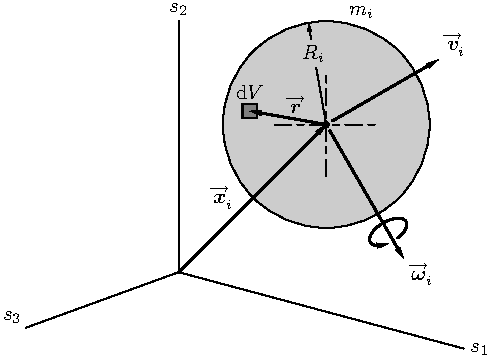
\includegraphics{figs/DEM-Def-Ball}
   \caption{Ball Element Parameters}
   \label{fig:BallDef}
\end{figure}


\subsection{Ball mass and inertia parameters}

Consider a volume element $\mathrm{d}V$ with respect to a static base $S$ of
an arbitrary solid body with  density $\rho$. The mass of the body is
obtained by integrating over the volume of the body,
\begin{equation}
    m = \int\limits_{\mathrm{body}} \rho\, \mathrm{d}V
    \label{eq:BMass-dif}
\end{equation}

In figure~\ref{fig:BallDef}, a ball with radius $R_{i}$ and uniform density
$\rho_i$ is depicted. The mass of the ball is after integration of
equation~\eqref{eq:BMass-dif}
\begin{equation}
    m_i = \tfrac{4}{3} \pi \rho_i\, R_i^3 .
    \label{eq:BMass}
\end{equation}


%----------------------------------------------------------------------------
\endinput

%\include{contents/App-2}
%\include{contents/App-3}

%==== Bibliography acro's & Index ===================================
\backmatter

\bibliography{backmatter/USbib-sample}

\end{document}
